\documentclass[11pt,a4paper]{article}

% --- Core LaTeX Packages ---
\usepackage[utf8]{inputenc}
\usepackage[T1]{fontenc}
\usepackage[margin=1in]{geometry}
\usepackage{amsmath,amssymb,amsthm}
\usepackage{xcolor}
\usepackage{listings}
\usepackage{hyperref}
\usepackage{tabularx}
\usepackage{xltabular}
\usepackage{array}
\usepackage{graphicx}
\usepackage{tikz}
\usetikzlibrary{arrows.meta,positioning,shapes.geometric,calc,fit,backgrounds,decorations.pathreplacing}

% --- Unified Color Palette ---
\definecolor{primaryblue}{RGB}{24, 75, 140}
\definecolor{codebg}{RGB}{248, 249, 250}
\definecolor{codeframe}{RGB}{210, 215, 222}
\definecolor{codegreen}{RGB}{40, 130, 60}
\definecolor{codeblue}{RGB}{20, 90, 180}
\definecolor{codegray}{RGB}{120, 120, 120}

% --- Hyperref Setup ---
\hypersetup{
    colorlinks=true,
    linkcolor=primaryblue,
    citecolor=primaryblue,
    urlcolor=primaryblue,
    pdftitle={Comprehensive Visual Diagram Review and Audit Gallery},
    pdfauthor={Antigravity Engineering}
}

% --- Callout Box Environment ---
\newenvironment{calloutbox}[1]{
    \par\vspace{0.3cm}
    \noindent\begin{tabular}{|p{0.96\textwidth}|}
    \hline
    \vspace{0.1cm}
    \textbf{#1}\par\vspace{0.1cm}
}{
    \vspace{0.1cm}
    \\ \hline
    \end{tabular}
    \vspace{0.3cm}\par
}

% --- Breadcrumb Command ---
\newcommand{\breadcrumb}[3]{
    \par\vspace{0.15cm}
    \noindent\begin{tabularx}{\textwidth}{|l|X|}
    \hline
    \textbf{Target Document:} & \texttt{\detokenize{#1}} \\
    \textbf{Target Placement:} & #2 \\
    \textbf{Pedagogical Purpose:} & #3 \\
    \hline
    \end{tabularx}
    \vspace{0.15cm}\par
}

% --- Diagram Review / Audit Table Command ---
\newcommand{\diagramaudit}[3]{
    \par\vspace{0.12cm}
    \noindent\begin{tabularx}{\textwidth}{|l|l|>{\raggedright\arraybackslash}X|}
    \hline
    \textbf{Reviewer (Human/Agent)} & \textbf{Date} & \textbf{What Was Fixed / Changed} \\ \hline
    #1 & #2 & #3 \\ \hline
    \end{tabularx}
    \vspace{0.12cm}\par
}

% --- Title Block ---
\title{\vspace{-1.5cm}\textbf{\Huge Unified Visual Diagram Review Gallery}\\[0.3cm]
\Large Comprehensive Visual Audit, Missing Diagram Analysis, and TikZ Architecture for the Algorithmic Library}
\author{Antigravity Engineering}
\date{\today}

\begin{document}

\maketitle

\begin{abstract}
\noindent
This document establishes the unified visual architecture for the entire 12-module algorithmic learning library. Designed specifically for visual learners who require spatial, mechanical intuition for foundational concepts as well as advanced algorithmic workflows, this review provides a comprehensive audit of all existing documents, catalogs explicit textual promises where diagrams were previously omitted, and showcases a complete gallery of 41 clean, scalable, standalone TikZ diagrams. Each diagram includes exact document destination breadcrumbs, section coordinates, and targeted pedagogical rationale.
\end{abstract}

\tableofcontents
\newpage

% ============================================================================
\section{Exhaustive Visual Audit of the Learning Materials Library}
% ============================================================================

A comprehensive line-by-line audit of all 12 modules currently residing in \texttt{learning\_materials/} reveals a fundamental disparity: while the mathematical prose and C++23 implementations adhere strictly to the repository standards, visual explanations are severely underutilized or left entirely unrendered. Most critically, several modules contain explicit textual promises of figures (e.g., ``Figure: Top-level triage tree'', ``This simple number line shows how integers map onto their remainders'', ``Below is a 4-node directed graph and its three C++ representations'') where the accompanying graphical environment was either left completely empty or omitted entirely.

\vspace{0.3cm}
\noindent
\begin{xltabular}{\textwidth}{|l|l|>{\raggedright\arraybackslash}X|}
\hline
\textbf{Module Source} & \textbf{Current Status} & \textbf{Audit Findings \& Detected Gaps} \\ \hline
\endfirsthead
\hline
\textbf{Module Source} & \textbf{Current Status} & \textbf{Audit Findings \& Detected Gaps} \\ \hline
\endhead
\hline
\endfoot
\hline
\endlastfoot
\texttt{00.cpp\_reference.tex} & Pure Text / Code & Zero diagrams. Missing foundational memory architecture: automatic stack vs dynamic heap layout, and \texttt{std::vector} capacity doubling reallocation. \\ \hline
\texttt{00.problem\_solving\_guide.tex} & Broken Placeholder & \textbf{Fatal Missing Figure}: Lines 113--119 contain an empty center block followed immediately by the caption \emph{Figure: Top-level triage tree}. \\ \hline
\texttt{01.combinatorics\_permutations.tex} & Pure Text / Formulas & Stars and Bars (Section 3.4) and Pascal's Triangle lattice walking (Section 2.2) lack visual spatial structures. Resolved in Diagram 4 and Diagram 40. \\ \hline
\texttt{02.modular\_arithmetic.tex} & Broken Placeholder & \textbf{Fatal Missing Figure}: Line 110 promises clock remainders without a diagram. Also missing repeated squaring exponentiation tree. Resolved in Diagram 5 and Diagram 38. \\ \hline
\texttt{03.number\_theory.tex} & Broken Placeholder & \textbf{Fatal Missing Figure}: Lines 390--394 announce Sieve of Eratosthenes with empty block. Lacks Euclidean rectangle tiling and divisor symmetry across $\sqrt{N}$. Resolved in Diagrams 6, 7, and 39. \\ \hline
\texttt{04.sequences\_and\_series.tex} & Pure Text & Prefix sums and difference arrays explained numerically but lack tape subtraction, impulse plots, and 2D subgrid inclusion-exclusion diagrams. Resolved in Diagrams 8, 9, 10, and 32. \\ \hline
\texttt{05.recursion\_and\_backtracking.tex} & 3 Broken Placeholders & \textbf{Fatal Missing Figures}: Line 131 announces \emph{recursion tree for $\text{fib}(4)$} with no drawing. Line 282 has \emph{Decision Tree for $n=2$:} followed by empty space. Line 294 has \emph{Decision Tree for Subsets:} followed by empty space. \\ \hline
\texttt{06.dynamic\_programming.tex} & Incomplete Trace & Lines 170--173 announce coin tables with blank lines. Lacks 0/1 knapsack space compression and LCS 2D matrix reconstruction. Resolved in Diagrams 13, 14, 33, and 34. \\ \hline
\texttt{07.graph\_algorithms.tex} & Broken Placeholder & \textbf{Fatal Missing Figure}: Lines 177--179 announce representation matrix without a graph. Lacks topological DAG ordering and bipartite odd-cycle proofs. Resolved in Diagrams 15, 16, 17, 18, 35, and 36. \\ \hline
\texttt{08.binary\_search.tex} & Truncated Trace & Section 2.1 introduces array $A$ without halving steps. Lacks rotated sorted array discontinuity bifurcation. Resolved in Diagrams 19, 20, and 37. \\ \hline
\texttt{09.string\_algorithms.tex} & Pure Text / Code & Zero diagrams in source. String matching, tries, KMP $\pi$-array fallbacks, and Rabin-Karp rolling hash shifts explained purely with formulas without visual state transitions. Covered in Diagrams 29, 30, and 31. \\ \hline
\texttt{10.greedy\_algorithms.tex} & 1 TikZ Figure & Contains interval scheduling timeline. Included below for unified review. \\ \hline
\texttt{11.monotonic\_stacks\_and\_queues.tex} & 3 TikZ Figures & Contains histogram expansion, cascading pops, and monotonic deque. Included below for unified review. \\ \hline
\texttt{12.bit\_manipulation\_and\_bitmasks.tex} & 5 TikZ Figures & Comprehensive 5-diagram visual architecture: Diagram 25 (Integer anatomy), Diagram 26 (Two's complement LSB isolation), Diagram 27 (Prefix XOR cancellation), Diagram 28 (Submask enumeration lattice), and Diagram 41 (Brian Kernighan's lowest set-bit stripping). Included below for unified review. \\ \hline
\end{xltabular}
\vspace{0.3cm}

\newpage
% ============================================================================
\section{Module 00: C++ Reference \& Architecture}
% ============================================================================

\subsection{Diagram 1: Memory Layout --- Automatic Stack vs Dynamic Heap Allocation}

\breadcrumb{00.cpp_reference.tex}{Section 9: Memory, Non-Owning Views, and Smart Pointers}{Demystifies pointer dereferencing, local variable scope, and the mechanical distinction between stack-allocated objects and heap-allocated buffers.}

\diagramaudit{Agent (Antigravity)}{2026-10-11}{Standardized layout across full text width ($15.5\text{ cm}$); aligned stack frames and heap buffers side-by-side; validated scalar and vector metadata byte sizes; calibrated pointer dereference and memory management vectors to prevent overlap with stack growth arrow.}

\begin{figure}[htbp]
\centering
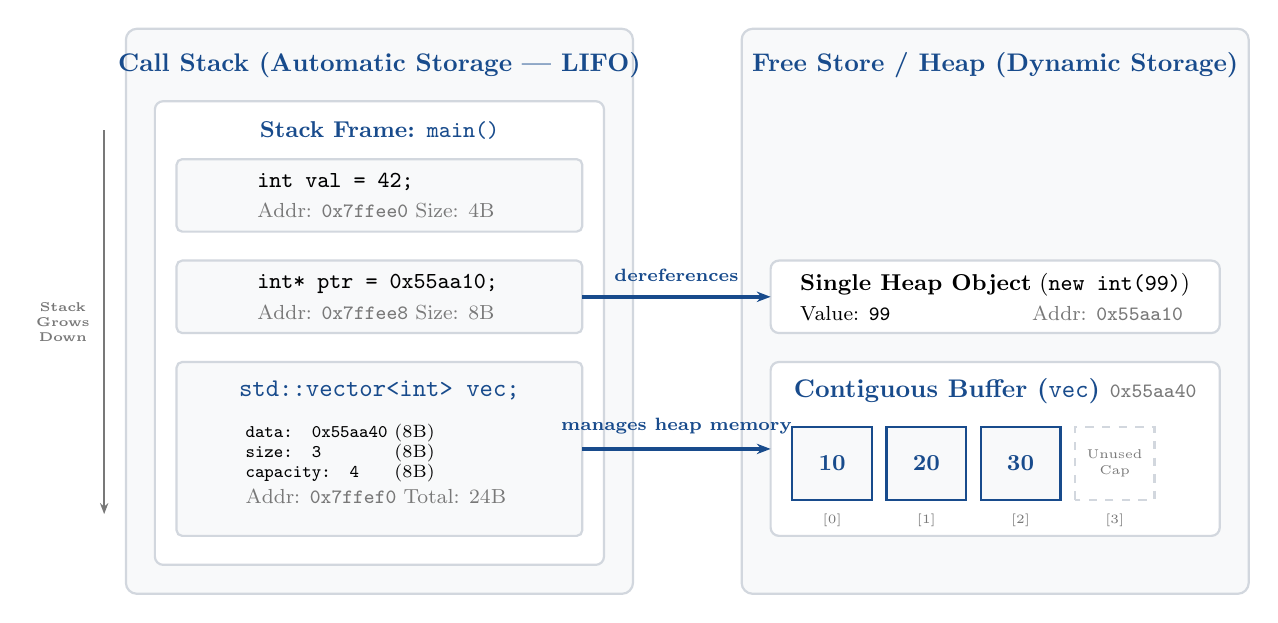
\begin{tikzpicture}[scale=0.92, every node/.style={transform shape}]
    % Memory regions container spanning textwidth (~15.5cm)
    \draw[thick, draw=codeframe, fill=codebg, rounded corners=4pt] (0, -0.6) rectangle (7.0, 7.2);
    \node[font=\bfseries\normalsize, primaryblue] at (3.5, 6.7) {Call Stack (Automatic Storage --- LIFO)};

    \draw[thick, draw=codeframe, fill=codebg, rounded corners=4pt] (8.5, -0.6) rectangle (15.5, 7.2);
    \node[font=\bfseries\normalsize, primaryblue] at (12.0, 6.7) {Free Store / Heap (Dynamic Storage)};

    % Stack Frames
    \draw[thick, draw=codeframe, fill=white, rounded corners=3pt] (0.4, -0.2) rectangle (6.6, 6.2);
    \node[font=\bfseries\small, primaryblue] at (3.5, 5.8) {Stack Frame: \texttt{main()}};

    % Stack Variables
    \draw[thick, draw=codeframe, fill=codebg, rounded corners=2pt] (0.7, 4.4) rectangle (6.3, 5.4);
    \node[font=\small, align=left] at (3.5, 4.9) {
        \texttt{int val = 42;}\\[1pt]
        \footnotesize\color{codegray}Addr: \texttt{0x7ffee0} \hfill Size: 4B
    };

    \draw[thick, draw=codeframe, fill=codebg, rounded corners=2pt] (0.7, 3.0) rectangle (6.3, 4.0);
    \node[font=\small, align=left] at (3.5, 3.5) {
        \texttt{int* ptr = 0x55aa10;}\\[1pt]
        \footnotesize\color{codegray}Addr: \texttt{0x7ffee8} \hfill Size: 8B
    };

    \draw[thick, draw=codeframe, fill=codebg, rounded corners=2pt] (0.7, 0.2) rectangle (6.3, 2.6);
    \node[font=\small, primaryblue, font=\bfseries] at (3.5, 2.2) {\texttt{std::vector<int> vec;}};
    \node[font=\scriptsize, align=left] at (3.5, 1.2) {
        \texttt{data:     0x55aa40} \hfill (8B)\\
        \texttt{size:     3} \hfill (8B)\\
        \texttt{capacity: 4} \hfill (8B)\\[2pt]
        \footnotesize\color{codegray}Addr: \texttt{0x7ffef0} \hfill Total: 24B
    };

    % Heap Allocations
    \draw[thick, draw=codeframe, fill=white, rounded corners=3pt] (8.9, 3.0) rectangle (15.1, 4.0);
    \node[font=\small, align=left] at (12.0, 3.5) {
        \textbf{Single Heap Object} (\texttt{new int(99)})\\[1pt]
        \footnotesize Value: \texttt{99} \hfill \color{codegray}Addr: \texttt{0x55aa10}
    };

    \draw[thick, draw=codeframe, fill=white, rounded corners=3pt] (8.9, 0.2) rectangle (15.1, 2.6);
    \node[font=\small, primaryblue, font=\bfseries] at (12.0, 2.2) {Contiguous Buffer (\texttt{vec}) \hfill \footnotesize\normalfont\color{codegray}\texttt{0x55aa40}};

    % Array slots in heap
    \foreach \i/\val in {0/10, 1/20, 2/30} {
        \draw[thick, draw=primaryblue, fill=codebg] (9.2 + \i*1.3, 0.7) rectangle (10.3 + \i*1.3, 1.7)
            node[midway, font=\small\bfseries, primaryblue] {\val};
        \node[font=\tiny, codegray, below=2pt] at (9.75 + \i*1.3, 0.7) {[\i]};
    }
    \draw[thick, dashed, draw=codeframe, fill=white] (13.1, 0.7) rectangle (14.2, 1.7)
        node[midway, font=\tiny, codegray, align=center] {Unused\\Cap};
    \node[font=\tiny, codegray, below=2pt] at (13.65, 0.7) {[3]};

    % Pointer Arrows
    \draw[->, line width=1.3pt, primaryblue, -{Stealth[length=5pt]}] (6.3, 3.5) -- (8.9, 3.5)
        node[midway, above=2pt, font=\scriptsize\bfseries, primaryblue] {dereferences};
    \draw[->, line width=1.3pt, primaryblue, -{Stealth[length=5pt]}] (6.3, 1.4) -- (8.9, 1.4)
        node[midway, above=2pt, font=\scriptsize\bfseries, primaryblue] {manages heap memory};

    % Stack Growth Direction
    \draw[->, thick, codegray, -{Stealth[length=4pt]}] (-0.3, 5.8) -- (-0.3, 0.5)
        node[midway, left=2pt, font=\tiny\bfseries, codegray, align=center] {Stack\\Grows\\Down};
\end{tikzpicture}
\caption{Memory layout showing stack frame storage for local scalar variables and vector control structures pointing to dynamically allocated heap buffers.}
\end{figure}

\newpage
\subsection{Diagram 2: \texttt{std::vector} Capacity Doubling and Reallocation}

\breadcrumb{00.cpp_reference.tex}{Section 1.1: Sequence Containers (std::vector)}{Visualizes geometric reallocation ($C \to 2C$), element copying overhead, pointer invalidation risks, and amortized $O(1)$ push\_back.}

\diagramaudit{Agent (Antigravity)}{2026-10-11}{Repositioned pointer invalidation warning box with non-overlapping dashed arrow; calibrated geometric doubling transition banner ($C \to 2C$); styled copied vs freshly inserted elements with distinct green stroke/fill; added amortized $O(1)$ guarantee proof card.}

\begin{figure}[htbp]
\centering
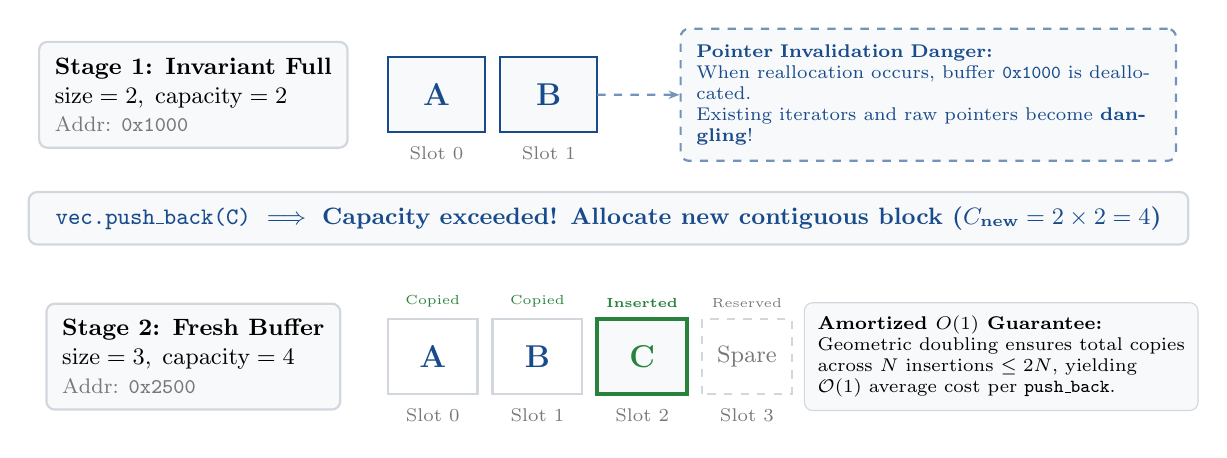
\begin{tikzpicture}[scale=0.95, every node/.style={transform shape}]
    % Stage 1: Full vector
    \node[draw=codeframe, fill=codebg, rounded corners=3pt, thick, align=left, font=\small, inner sep=6pt] at (2.2, 4.5) {
        \textbf{Stage 1: Invariant Full}\\
        $\text{size} = 2, \; \text{capacity} = 2$\\
        \footnotesize\color{codegray}Addr: \texttt{0x1000}
    };

    % Slots in old buffer
    \foreach \i/\val in {0/A, 1/B} {
        \draw[thick, draw=primaryblue, fill=codebg] (4.8 + \i*1.5, 4.0) rectangle (6.1 + \i*1.5, 5.0)
            node[midway, font=\large\bfseries, primaryblue] {\val};
        \node[font=\scriptsize, codegray, below=2pt] at (5.45 + \i*1.5, 4.0) {Slot \i};
    }

    % Warning box on the right
    \node[draw=primaryblue!60, fill=codebg, thick, dashed, rounded corners=3pt, font=\scriptsize, align=left, text width=6.2cm, inner sep=6pt, anchor=west] (inval) at (8.7, 4.5) {
        \color{primaryblue}\textbf{Pointer Invalidation Danger:}\\
        When reallocation occurs, buffer \texttt{0x1000} is deallocated.\\
        Existing iterators and raw pointers become \textbf{dangling}!
    };
    \draw[->, thick, primaryblue!60, dashed, -{Stealth[length=4pt]}] (7.6, 4.5) -- (inval.west);

    % Action transition banner across page
    \draw[draw=codeframe, fill=codebg, rounded corners=3pt, thick] (0, 2.5) rectangle (15.5, 3.2);
    \node[font=\small\bfseries, primaryblue] at (7.75, 2.85) {
        \texttt{vec.push\_back(C)} $\implies$ Capacity exceeded! Allocate new contiguous block ($C_{\text{new}} = 2 \times 2 = 4$)
    };

    % Stage 2: Fresh block allocated
    \node[draw=codeframe, fill=codebg, rounded corners=3pt, thick, align=left, font=\small, inner sep=6pt] at (2.2, 1.0) {
        \textbf{Stage 2: Fresh Buffer}\\
        $\text{size} = 3, \; \text{capacity} = 4$\\
        \footnotesize\color{codegray}Addr: \texttt{0x2500}
    };

    % Slots in new buffer
    \foreach \i/\val in {0/A, 1/B} {
        \draw[thick, draw=codeframe, fill=white] (4.8 + \i*1.4, 0.5) rectangle (6.0 + \i*1.4, 1.5)
            node[midway, font=\large\bfseries, primaryblue] {\val};
        \node[font=\tiny, codegreen, above=1pt] at (5.4 + \i*1.4, 1.5) {Copied};
        \node[font=\scriptsize, codegray, below=2pt] at (5.4 + \i*1.4, 0.5) {Slot \i};
    }

    % Inserted slot C
    \draw[line width=1.5pt, draw=codegreen, fill=codebg] (7.6, 0.5) rectangle (8.8, 1.5)
        node[midway, font=\large\bfseries, codegreen] {C};
    \node[font=\tiny\bfseries, codegreen, above=1pt] at (8.2, 1.5) {Inserted};
    \node[font=\scriptsize, codegray, below=2pt] at (8.2, 0.5) {Slot 2};

    % Spare capacity slot
    \draw[thick, dashed, draw=codeframe, fill=white] (9.0, 0.5) rectangle (10.2, 1.5)
        node[midway, font=\small, codegray] {Spare};
    \node[font=\tiny, codegray, above=1pt] at (9.6, 1.5) {Reserved};
    \node[font=\scriptsize, codegray, below=2pt] at (9.6, 0.5) {Slot 3};

    % Amortized explanation card
    \node[draw=codeframe, fill=codebg, rounded corners=3pt, font=\scriptsize, align=left, inner sep=5pt] at (13.0, 1.0) {
        \textbf{Amortized $O(1)$ Guarantee:}\\
        Geometric doubling ensures total copies\\
        across $N$ insertions $\le 2N$, yielding\\
        $\mathcal{O}(1)$ average cost per \texttt{push\_back}.
    };
\end{tikzpicture}
\caption{Visualizing dynamic array geometric reallocation: allocating new contiguous heap storage of double capacity, copying existing elements, appending the incoming value, and deallocating the obsolete memory.}
\end{figure}

\newpage
% ============================================================================
\section{Module 00: Master Problem-Solving Decision Guide}
% ============================================================================

\subsection{Diagram 3: Top-Level Algorithmic Triage Decision Tree}

\breadcrumb{00.problem_solving_guide.tex}{Section 1: Step 1: Identify What the Problem Asks For (replaces missing figure at lines 113--119)}{Eliminates the empty figure placeholder and establishes the five primary objective branches: Optimization, Enumeration, Decision, Counting, and Querying.}

\diagramaudit{Agent (Antigravity)}{2026-10-11}{Replaced broken placeholder with 5 balanced columns (Optimization, Enumeration, Decision, Counting, Querying) spanning full $15.2\text{ cm}$ width; calibrated column widths ($2.85\text{ cm}$) to eliminate text clipping; aligned triage arrows directly into category card headers.}

\begin{figure}[htbp]
\centering
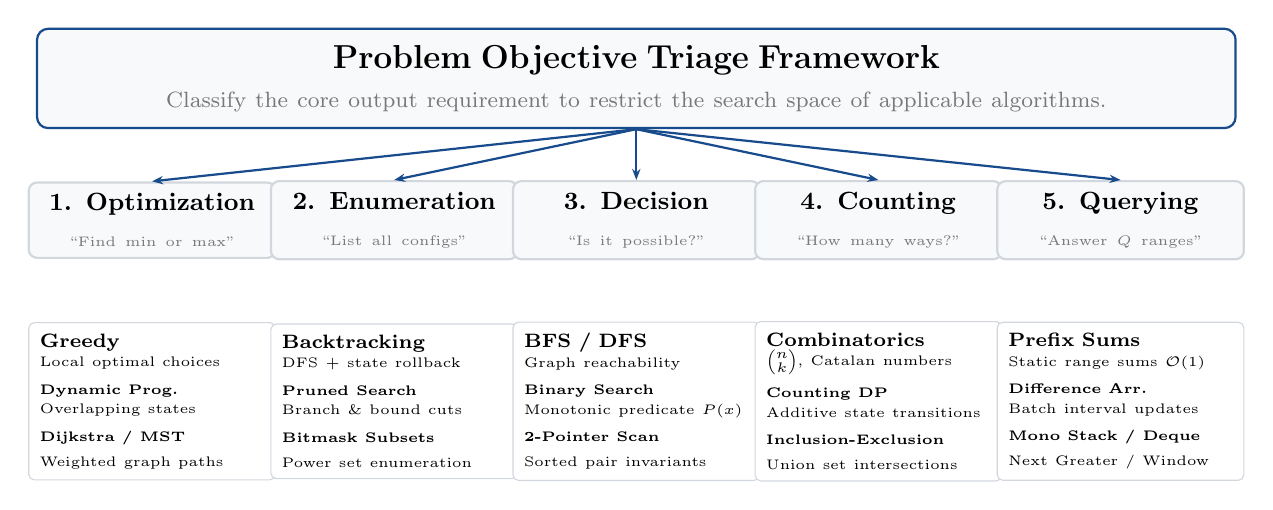
\begin{tikzpicture}[every node/.style={transform shape}]
    % Root Banner spanning full width
    \node[draw=primaryblue, fill=codebg, rounded corners=4pt, thick, align=center, inner sep=6pt, text width=14.8cm] (root) at (7.6, 7.5) {
        \textbf{\large Problem Objective Triage Framework}\\[2pt]
        \footnotesize\color{codegray}Classify the core output requirement to restrict the search space of applicable algorithms.
    };

    % 5 Balanced Columns across 15.2cm width (width=2.85cm each)
    % Col 1: Optimization (x = 1.45)
    \node[draw=codeframe, fill=codebg, rounded corners=3pt, thick, align=center, inner sep=4pt, text width=2.85cm] (c1) at (1.45, 5.7) {
        \textbf{\small 1. Optimization}\\[1pt]
        \tiny\color{codegray}``Find $\min$ or $\max$''
    };
    \draw[->, thick, primaryblue, -{Stealth[length=4pt]}] (root.south) -- (c1.north);

    \node[draw=codeframe, fill=white, rounded corners=2pt, align=left, font=\scriptsize, text width=2.85cm, inner sep=4pt] at (1.45, 3.4) {
        \textbf{Greedy}\\[1pt]
        \tiny Local optimal choices\\[4pt]
        \textbf{Dynamic Prog.}\\[1pt]
        \tiny Overlapping states\\[4pt]
        \textbf{Dijkstra / MST}\\[1pt]
        \tiny Weighted graph paths
    };

    % Col 2: Enumeration (x = 4.525)
    \node[draw=codeframe, fill=codebg, rounded corners=3pt, thick, align=center, inner sep=4pt, text width=2.85cm] (c2) at (4.525, 5.7) {
        \textbf{\small 2. Enumeration}\\[1pt]
        \tiny\color{codegray}``List all configs''
    };
    \draw[->, thick, primaryblue, -{Stealth[length=4pt]}] (root.south) -- (c2.north);

    \node[draw=codeframe, fill=white, rounded corners=2pt, align=left, font=\scriptsize, text width=2.85cm, inner sep=4pt] at (4.525, 3.4) {
        \textbf{Backtracking}\\[1pt]
        \tiny DFS + state rollback\\[4pt]
        \textbf{Pruned Search}\\[1pt]
        \tiny Branch \& bound cuts\\[4pt]
        \textbf{Bitmask Subsets}\\[1pt]
        \tiny Power set enumeration
    };

    % Col 3: Decision (x = 7.6)
    \node[draw=codeframe, fill=codebg, rounded corners=3pt, thick, align=center, inner sep=4pt, text width=2.85cm] (c3) at (7.6, 5.7) {
        \textbf{\small 3. Decision}\\[1pt]
        \tiny\color{codegray}``Is it possible?''
    };
    \draw[->, thick, primaryblue, -{Stealth[length=4pt]}] (root.south) -- (c3.north);

    \node[draw=codeframe, fill=white, rounded corners=2pt, align=left, font=\scriptsize, text width=2.85cm, inner sep=4pt] at (7.6, 3.4) {
        \textbf{BFS / DFS}\\[1pt]
        \tiny Graph reachability\\[4pt]
        \textbf{Binary Search}\\[1pt]
        \tiny Monotonic predicate $P(x)$\\[4pt]
        \textbf{2-Pointer Scan}\\[1pt]
        \tiny Sorted pair invariants
    };

    % Col 4: Counting (x = 10.675)
    \node[draw=codeframe, fill=codebg, rounded corners=3pt, thick, align=center, inner sep=4pt, text width=2.85cm] (c4) at (10.675, 5.7) {
        \textbf{\small 4. Counting}\\[1pt]
        \tiny\color{codegray}``How many ways?''
    };
    \draw[->, thick, primaryblue, -{Stealth[length=4pt]}] (root.south) -- (c4.north);

    \node[draw=codeframe, fill=white, rounded corners=2pt, align=left, font=\scriptsize, text width=2.85cm, inner sep=4pt] at (10.675, 3.4) {
        \textbf{Combinatorics}\\[1pt]
        \tiny $\binom{n}{k}$, Catalan numbers\\[4pt]
        \textbf{Counting DP}\\[1pt]
        \tiny Additive state transitions\\[4pt]
        \textbf{Inclusion-Exclusion}\\[1pt]
        \tiny Union set intersections
    };

    % Col 5: Querying (x = 13.75)
    \node[draw=codeframe, fill=codebg, rounded corners=3pt, thick, align=center, inner sep=4pt, text width=2.85cm] (c5) at (13.75, 5.7) {
        \textbf{\small 5. Querying}\\[1pt]
        \tiny\color{codegray}``Answer $Q$ ranges''
    };
    \draw[->, thick, primaryblue, -{Stealth[length=4pt]}] (root.south) -- (c5.north);

    \node[draw=codeframe, fill=white, rounded corners=2pt, align=left, font=\scriptsize, text width=2.85cm, inner sep=4pt] at (13.75, 3.4) {
        \textbf{Prefix Sums}\\[1pt]
        \tiny Static range sums $\mathcal{O}(1)$\\[4pt]
        \textbf{Difference Arr.}\\[1pt]
        \tiny Batch interval updates\\[4pt]
        \textbf{Mono Stack / Deque}\\[1pt]
        \tiny Next Greater / Window
    };
\end{tikzpicture}
\caption{The top-level algorithmic triage decision architecture. Categorizing the core answer format immediately identifies the feasible algorithmic paradigms.}
\end{figure}

\newpage
% ============================================================================
\section{Module 01: Combinatorics and Permutations}
% ============================================================================

\subsection{Diagram 4: Stars and Bars Partitioning Model}

\breadcrumb{01.combinatorics_permutations.tex}{Section 3.4: Combinations with Repetition (Stars and Bars)}{Provides physical spatial intuition for mapping $n$ indistinguishable objects and $k$ bins to choosing $k-1$ divider positions among $n + k - 1$ total slots.}

\diagramaudit{Agent (Antigravity)}{2026-10-11}{Corrected condition logic to non-negative integer partitioning ($x_i \ge 0$); mapped $n=7$ stars and $k=3$ bins across 9 distinct slots ($n+k-1=9$); rendered filled divider bars; aligned bottom bin grouping braces; verified formula evaluation ($\binom{9}{2} = 36$).}

\begin{figure}[htbp]
\centering
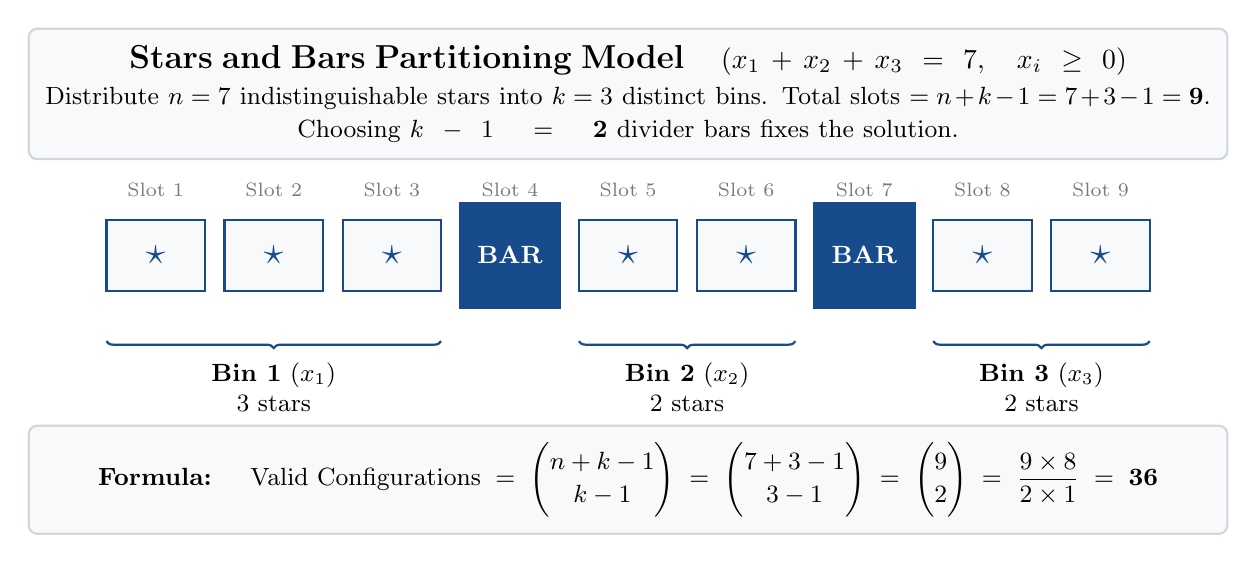
\begin{tikzpicture}[every node/.style={transform shape}]
    % Top Equation & Explanation Banner across full textwidth
    \node[draw=codeframe, fill=codebg, rounded corners=3pt, thick, align=center, inner sep=6pt, text width=14.8cm] at (7.6, 4.3) {
        \textbf{\large Stars and Bars Partitioning Model} \quad $(x_1 + x_2 + x_3 = 7, \quad x_i \ge 0)$\\[2pt]
        \small Distribute $n=7$ indistinguishable stars into $k=3$ distinct bins. Total slots $= n + k - 1 = 7 + 3 - 1 = \mathbf{9}$.\\
        Choosing $k-1 = \mathbf{2}$ divider bars fixes the solution.
    };

    % 9 slots centered across page (x from 0.975 to 14.225)
    \foreach \s/\isbar in {
        1/0, 2/0, 3/0,
        4/1,
        5/0, 6/0,
        7/1,
        8/0, 9/0
    } {
        \pgfmathsetmacro{\xpos}{0.975 + (\s - 1)*1.5}
        \ifnum\isbar=0
            \draw[thick, draw=primaryblue, fill=codebg] (\xpos, 1.8) rectangle (\xpos+1.25, 2.7);
            \node[font=\Large, primaryblue] at (\xpos+0.625, 2.25) {$\star$};
        \else
            \draw[line width=1.5pt, draw=primaryblue, fill=primaryblue] (\xpos, 1.6) rectangle (\xpos+1.25, 2.9);
            \node[font=\small\bfseries, text=white] at (\xpos+0.625, 2.25) {BAR};
        \fi
        \node[font=\scriptsize, codegray, above=2pt] at (\xpos+0.625, 2.8) {Slot \s};
    }

    % Bins underneath with braces
    \draw[thick, draw=primaryblue, decoration={brace, mirror, raise=4pt}, decorate] (0.975, 1.3) -- (5.225, 1.3)
        node[midway, below=8pt, font=\small, align=center] {\textbf{Bin 1} ($x_1$)\\3 stars};

    \draw[thick, draw=primaryblue, decoration={brace, mirror, raise=4pt}, decorate] (6.975, 1.3) -- (9.725, 1.3)
        node[midway, below=8pt, font=\small, align=center] {\textbf{Bin 2} ($x_2$)\\2 stars};

    \draw[thick, draw=primaryblue, decoration={brace, mirror, raise=4pt}, decorate] (11.475, 1.3) -- (14.225, 1.3)
        node[midway, below=8pt, font=\small, align=center] {\textbf{Bin 3} ($x_3$)\\2 stars};

    % Mathematical formula badge across full width
    \node[draw=codeframe, fill=codebg, rounded corners=3pt, thick, font=\small, inner sep=6pt, align=center, text width=14.8cm] at (7.6, -0.6) {
        \textbf{Formula:} \quad $\text{Valid Configurations} = \displaystyle\binom{n + k - 1}{k - 1} = \binom{7 + 3 - 1}{3 - 1} = \binom{9}{2} = \frac{9 \times 8}{2 \times 1} = \mathbf{36}$
    };
\end{tikzpicture}
\caption{Stars and Bars partitioning for $n=7$ items into $k=3$ distinct bins. Placing 2 bars into 9 slots uniquely partitions the 7 stars into three non-negative integer parts.}
\end{figure}

\newpage
% ============================================================================
\section{Module 02: Modular Arithmetic}
% ============================================================================

\subsection{Diagram 5: The Modular Arithmetic Clock Face (\texorpdfstring{$\mathbb{Z}_{12}$}{Z12})}

\breadcrumb{02.modular_arithmetic.tex}{Section 1.1: From Linear Numbers to Cyclic Systems (replaces missing figure at line 110)}{Replaces the omitted number line/clock figure promised in the text, illustrating additive wrap-around, remainder classes, and negative modulo reduction.}

\diagramaudit{Agent (Antigravity)}{2026-10-11}{Replaced broken placeholder at line 110; placed clock face (radius $2.2\text{ cm}$) in left panel and congruence classes card in right panel; calibrated addition arc (clockwise, $r=2.5\text{ cm}$) and subtraction arc (counter-clockwise, $r=3.1\text{ cm}$) to prevent path collision; added canonical C++ non-negative modulo rule.}

\begin{figure}[htbp]
\centering
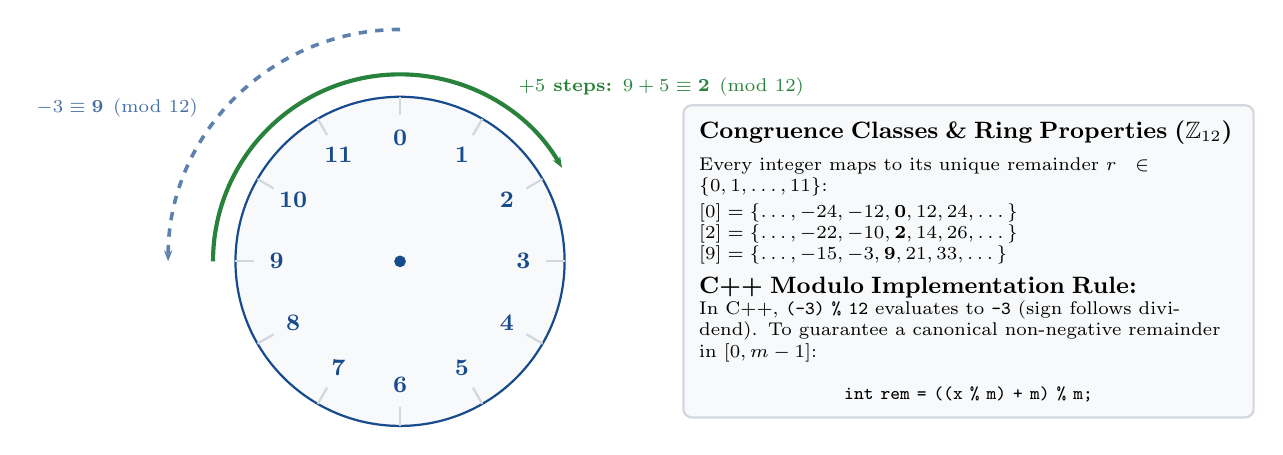
\begin{tikzpicture}[scale=0.95, every node/.style={transform shape}]
    % Left Panel: Modular Clock (x in 0 to 7.8)
    \begin{scope}[xshift=3.8cm, yshift=2.4cm]
        % Outer clock circle
        \draw[thick, draw=primaryblue, fill=codebg] (0, 0) circle (2.2);

        % Clock ticks and numbers 0..11
        \foreach \val/\deg in {
            0/90, 1/60, 2/30, 3/0, 4/-30, 5/-60, 6/-90, 7/-120, 8/-150, 9/-180, 10/-210, 11/-240
        } {
            \draw[thick, draw=codeframe] (\deg:1.95) -- (\deg:2.2);
            \node[font=\small\bfseries, primaryblue] at (\deg:1.65) {\val};
        }
        \filldraw[primaryblue] (0, 0) circle (2pt);

        % Addition arc: 9 + 5 = 14 = 2 (mod 12)
        \draw[->, line width=1.5pt, codegreen, -{Stealth[length=4pt]}] (180:2.5) arc (180:30:2.5);
        \node[codegreen, font=\scriptsize\bfseries, anchor=south west] at (55:2.55) {$+5$ steps: $9 + 5 \equiv \mathbf{2} \pmod{12}$};

        % Subtraction arc: 0 - 3 = 9 (mod 12) (counter-clockwise at radius 3.1)
        \draw[->, line width=1.3pt, primaryblue!70, dashed, -{Stealth[length=4pt]}] (90:3.1) arc (90:180:3.1);
        \node[primaryblue!80, font=\scriptsize\bfseries, anchor=south east] at (145:3.15) {$-3 \equiv \mathbf{9} \pmod{12}$};
    \end{scope}

    % Right Panel: Algebraic Reference Card (x in 7.6 to 15.2)
    \node[draw=codeframe, fill=codebg, rounded corners=3pt, thick, align=left, font=\scriptsize, inner sep=6pt, text width=7.2cm] at (11.4, 2.4) {
        \textbf{\small Congruence Classes \& Ring Properties ($\mathbb{Z}_{12}$)}\\[4pt]
        Every integer maps to its unique remainder $r \in \{0, 1, \dots, 11\}$:\\[2pt]
        $[0] = \{\dots, -24, -12, \mathbf{0}, 12, 24, \dots\}$\\
        $[2] = \{\dots, -22, -10, \mathbf{2}, 14, 26, \dots\}$\\
        $[9] = \{\dots, -15, -3, \mathbf{9}, 21, 33, \dots\}$\\[5pt]
        \textbf{\small C++ Modulo Implementation Rule:}\\
        In C++, \texttt{(-3) \% 12} evaluates to \texttt{-3} (sign follows dividend). To guarantee a canonical non-negative remainder in $[0, m-1]$:
        \begin{center}
        \texttt{int rem = ((x \% m) + m) \% m;}
        \end{center}
    };
\end{tikzpicture}
\caption{The modular arithmetic clock face ($\mathbb{Z}_{12}$). Numbers wrap periodically around the finite circle. Moving clockwise models addition; moving counter-clockwise models subtraction.}
\end{figure}

\newpage
% ============================================================================
\section{Module 03: Number Theory}
% ============================================================================

\subsection{Diagram 6: Sieve of Eratosthenes Composite Elimination Matrix}

\breadcrumb{03.number_theory.tex}{Section 3.1: Pattern 1: Sieve of Eratosthenes (replaces missing trace at lines 390--394)}{Fulfills the empty trace placeholder for $N=30$. Clearly demonstrates why multiples of prime $p$ only need to be eliminated starting from $p^2$.}

\diagramaudit{Agent (Antigravity)}{2026-10-11}{Replaced broken trace placeholder at lines 390--394 for $N=30$; formatted numbers 1--30 into a $5 \times 6$ matrix; highlighted surviving primes in bold blue; rendered diagonal strike-outs for composites; added elimination progression panel demonstrating $p^2$ jump starts and $\lfloor\sqrt{30}\rfloor=5$ termination.}

\begin{figure}[htbp]
\centering
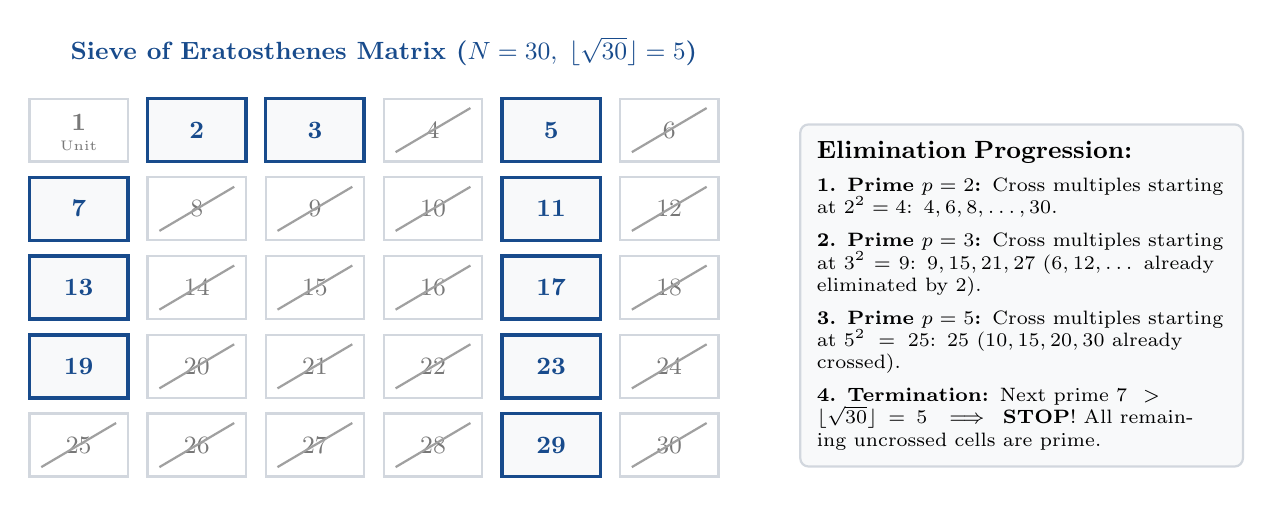
\begin{tikzpicture}[every node/.style={transform shape}]
    % Title across left panel
    \node[font=\bfseries\small, primaryblue] at (4.5, 5.6) {Sieve of Eratosthenes Matrix ($N = 30, \; \lfloor\sqrt{30}\rfloor = 5$)};

    % 5 rows x 6 cols grid for 1..30 (x in 0.0 to 9.2)
    \foreach \n in {1,2,...,30} {
        \pgfmathtruncatemacro{\col}{mod(\n-1, 6)}
        \pgfmathtruncatemacro{\row}{int((\n-1)/6)}
        \pgfmathsetmacro{\x}{\col * 1.5}
        \pgfmathsetmacro{\y}{4.2 - \row * 1.0}

        \ifnum\n=1
            % Unit: 1
            \draw[thick, draw=codeframe, fill=white] (\x, \y) rectangle (\x+1.25, \y+0.8);
            \node[font=\small\bfseries, codegray] at (\x+0.625, \y+0.5) {\n};
            \node[font=\tiny, codegray] at (\x+0.625, \y+0.2) {Unit};
        \else\ifnum\n=2
            \draw[line width=1.3pt, draw=primaryblue, fill=codebg] (\x, \y) rectangle (\x+1.25, \y+0.8);
            \node[font=\small\bfseries, primaryblue] at (\x+0.625, \y+0.4) {\n};
        \else\ifnum\n=3
            \draw[line width=1.3pt, draw=primaryblue, fill=codebg] (\x, \y) rectangle (\x+1.25, \y+0.8);
            \node[font=\small\bfseries, primaryblue] at (\x+0.625, \y+0.4) {\n};
        \else\ifnum\n=5
            \draw[line width=1.3pt, draw=primaryblue, fill=codebg] (\x, \y) rectangle (\x+1.25, \y+0.8);
            \node[font=\small\bfseries, primaryblue] at (\x+0.625, \y+0.4) {\n};
        \else\ifnum\n=7
            \draw[line width=1.3pt, draw=primaryblue, fill=codebg] (\x, \y) rectangle (\x+1.25, \y+0.8);
            \node[font=\small\bfseries, primaryblue] at (\x+0.625, \y+0.4) {\n};
        \else\ifnum\n=11
            \draw[line width=1.3pt, draw=primaryblue, fill=codebg] (\x, \y) rectangle (\x+1.25, \y+0.8);
            \node[font=\small\bfseries, primaryblue] at (\x+0.625, \y+0.4) {\n};
        \else\ifnum\n=13
            \draw[line width=1.3pt, draw=primaryblue, fill=codebg] (\x, \y) rectangle (\x+1.25, \y+0.8);
            \node[font=\small\bfseries, primaryblue] at (\x+0.625, \y+0.4) {\n};
        \else\ifnum\n=17
            \draw[line width=1.3pt, draw=primaryblue, fill=codebg] (\x, \y) rectangle (\x+1.25, \y+0.8);
            \node[font=\small\bfseries, primaryblue] at (\x+0.625, \y+0.4) {\n};
        \else\ifnum\n=19
            \draw[line width=1.3pt, draw=primaryblue, fill=codebg] (\x, \y) rectangle (\x+1.25, \y+0.8);
            \node[font=\small\bfseries, primaryblue] at (\x+0.625, \y+0.4) {\n};
        \else\ifnum\n=23
            \draw[line width=1.3pt, draw=primaryblue, fill=codebg] (\x, \y) rectangle (\x+1.25, \y+0.8);
            \node[font=\small\bfseries, primaryblue] at (\x+0.625, \y+0.4) {\n};
        \else\ifnum\n=29
            \draw[line width=1.3pt, draw=primaryblue, fill=codebg] (\x, \y) rectangle (\x+1.25, \y+0.8);
            \node[font=\small\bfseries, primaryblue] at (\x+0.625, \y+0.4) {\n};
        \else
            % Composite numbers crossed out with subtle slash
            \draw[thick, draw=codeframe, fill=white] (\x, \y) rectangle (\x+1.25, \y+0.8);
            \node[font=\small, codegray] at (\x+0.625, \y+0.4) {\n};
            \draw[thick, codegray!70] (\x+0.15, \y+0.12) -- (\x+1.1, \y+0.68);
        \fi\fi\fi\fi\fi\fi\fi\fi\fi\fi\fi
    }

    % Right Panel: Elimination Trace & Principle Card (x in 9.8 to 15.5)
    \node[draw=codeframe, fill=codebg, rounded corners=3pt, thick, align=left, font=\scriptsize, inner sep=6pt, text width=5.2cm] at (12.6, 2.5) {
        \textbf{\small Elimination Progression:}\\[4pt]
        \textbf{1. Prime $p=2$:} Cross multiples starting at $2^2 = 4$: $4, 6, 8, \dots, 30$.\\[4pt]
        \textbf{2. Prime $p=3$:} Cross multiples starting at $3^2 = 9$: $9, 15, 21, 27$ ($6, 12, \dots$ already eliminated by 2).\\[4pt]
        \textbf{3. Prime $p=5$:} Cross multiples starting at $5^2 = 25$: $25$ ($10, 15, 20, 30$ already crossed).\\[4pt]
        \textbf{4. Termination:} Next prime $7 > \lfloor\sqrt{30}\rfloor = 5 \implies$ \textbf{STOP}! All remaining uncrossed cells are prime.
    };
\end{tikzpicture}
\caption{Sieve of Eratosthenes elimination matrix for $N=30$. Highlighted cells denote surviving primes. Crossed cells represent composite values eliminated by primes $p \le \sqrt{30}$.}
\end{figure}

\newpage
\subsection{Diagram 7: Euclidean Algorithm Geometric Rectangle Tiling}

\breadcrumb{03.number_theory.tex}{Section 2.3: The Euclidean Algorithm (callout box lines 255--257)}{Renders the geometric proof of why $\gcd(a, b) = \gcd(b, a \bmod b)$ through successive square packing of a $252 \times 105$ rectangle.}

\diagramaudit{Agent (Antigravity)}{2026-10-11}{Replaced text-only description with geometric $252 \times 105$ square tiling; nested two $105 \times 105$ squares, two $42 \times 42$ squares, and two $21 \times 21$ final GCD squares; separated dimension annotations to prevent label crowding; verified reduction chain badge $\gcd(252, 105) = 21$.}

\begin{figure}[htbp]
\centering
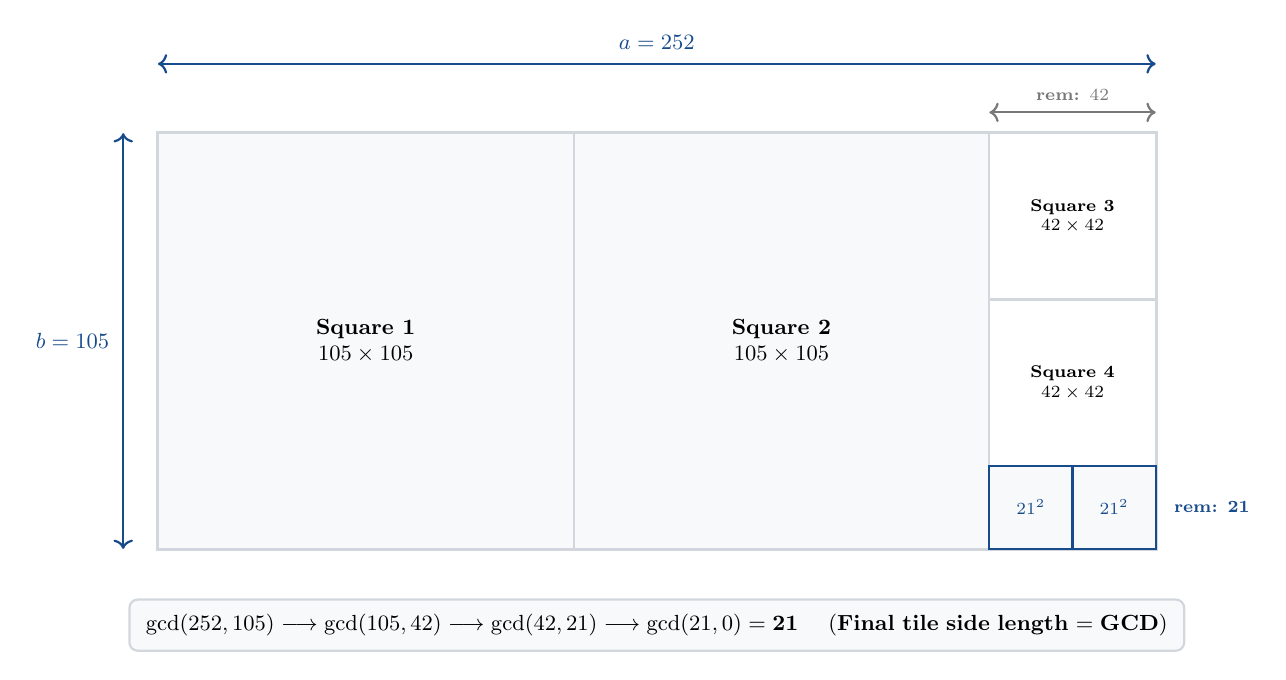
\begin{tikzpicture}[scale=0.88, every node/.style={transform shape}]
    % Outer rectangle: 252 x 105. Scaled width = 14.4cm, height = 6.0cm
    % Square 1 (105x105): 6.0cm x 6.0cm (x = 0.5 to 6.5)
    % Square 2 (105x105): 6.0cm x 6.0cm (x = 6.5 to 12.5)
    % Remainder (42x105): width 2.4cm (x = 12.5 to 14.9)
    %   Square 3 (42x42): height 2.4cm (y = 4.1 to 6.5)
    %   Square 4 (42x42): height 2.4cm (y = 1.7 to 4.1)
    %   Remainder (42x21): height 1.2cm (y = 0.5 to 1.7)
    %     Tile 1 (21x21): width 1.2cm (x = 12.5 to 13.7)
    %     Tile 2 (21x21): width 1.2cm (x = 13.7 to 14.9)

    % Base rectangle frame
    \draw[line width=1.5pt, draw=codeframe] (0.5, 0.5) rectangle (14.9, 6.5);

    % Step 1: Two 105 x 105 squares
    \draw[thick, draw=codeframe, fill=codebg] (0.5, 0.5) rectangle (6.5, 6.5)
        node[midway, align=center, font=\small] {\textbf{Square 1}\\$105 \times 105$};
    \draw[thick, draw=codeframe, fill=codebg] (6.5, 0.5) rectangle (12.5, 6.5)
        node[midway, align=center, font=\small] {\textbf{Square 2}\\$105 \times 105$};

    % Step 2: Two 42 x 42 squares
    \draw[thick, draw=codeframe, fill=white] (12.5, 4.1) rectangle (14.9, 6.5)
        node[midway, align=center, font=\scriptsize] {\textbf{Square 3}\\$42 \times 42$};
    \draw[thick, draw=codeframe, fill=white] (12.5, 1.7) rectangle (14.9, 4.1)
        node[midway, align=center, font=\scriptsize] {\textbf{Square 4}\\$42 \times 42$};

    % Step 3: Two 21 x 21 squares (final GCD tiles)
    \draw[thick, draw=primaryblue, fill=codebg] (12.5, 0.5) rectangle (13.7, 1.7)
        node[midway, font=\scriptsize\bfseries, primaryblue] {$21^2$};
    \draw[thick, draw=primaryblue, fill=codebg] (13.7, 0.5) rectangle (14.9, 1.7)
        node[midway, font=\scriptsize\bfseries, primaryblue] {$21^2$};

    % Dimensions annotations
    \draw[<->, thick, primaryblue] (0.5, 7.5) -- (14.9, 7.5)
        node[midway, above=2pt, font=\small\bfseries] {$a = 252$};
    \draw[<->, thick, primaryblue] (0.0, 0.5) -- (0.0, 6.5)
        node[midway, left=2pt, font=\small\bfseries] {$b = 105$};

    \draw[<->, thick, codegray] (12.5, 6.8) -- (14.9, 6.8)
        node[midway, above=1pt, font=\scriptsize\bfseries, codegray] {rem: $42$};
    \node[right=4pt, font=\scriptsize\bfseries, primaryblue] at (14.9, 1.1) {rem: $\mathbf{21}$};

    % Bottom Reduction Badge across full width
    \node[draw=codeframe, fill=codebg, rounded corners=3pt, thick, font=\small, inner sep=6pt, align=center, text width=14.8cm] at (7.7, -0.6) {
        $\gcd(252, 105) \longrightarrow \gcd(105, 42) \longrightarrow \gcd(42, 21) \longrightarrow \gcd(21, 0) = \mathbf{21}$ \quad (\textbf{Final tile side length} $= \mathbf{GCD}$)
    };
\end{tikzpicture}
\caption{Euclidean rectangle tiling for $252 \times 105$. Successively packing maximal squares mirrors the algebraic modulo reductions until the area is perfectly tiled by $21 \times 21$ squares.}
\end{figure}

\newpage
% ============================================================================
\section{Module 04: Sequences, Series, and Range Queries}
% ============================================================================

\subsection{Diagram 8: 1D Prefix Sum Cumulative Tape \& Range Query Deconstruction}

\breadcrumb{04.sequences_and_series.tex}{Section 3.1: Prefix Sums for Range Queries in O(1)}{Visualizes array prefix accumulation and the exact subtraction mechanism $P[R+1] - P[L]$ that yields subarray sums in $O(1)$.}

\diagramaudit{Agent (Antigravity)}{2026-10-11}{Aligned original array $A$ directly above prefix array $P$; highlighted query interval $[2 \dots 4]$ with dashed bounding box; routed downward curved Bezier arrows from $P[2]$ and $P[5]$ into $O(1)$ subtraction formula badge to eliminate cell crossing; verified sum evaluation ($14 - 4 = 10$).}

\begin{figure}[htbp]
\centering
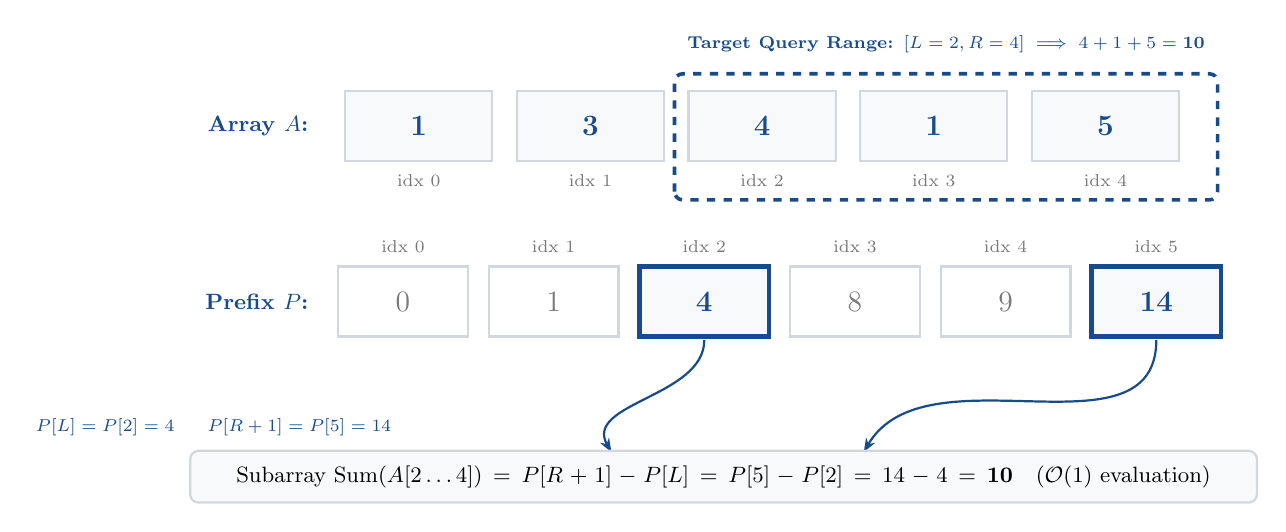
\begin{tikzpicture}[scale=0.89, every node/.style={transform shape}]
    % Top Row: Original Array A (x spanning 0.5 to 15.0)
    \node[font=\bfseries\small, primaryblue, anchor=east] at (1.8, 4.3) {Array $A$:};

    % 5 boxes for A[0..4], each width 2.1cm, spacing 0.35cm
    \foreach \i/\val in {0/1, 1/3, 2/4, 3/1, 4/5} {
        \pgfmathsetmacro{\xpos}{2.2 + \i * 2.45}
        \draw[thick, draw=codeframe, fill=codebg] (\xpos, 3.8) rectangle (\xpos+2.1, 4.8);
        \node[font=\large\bfseries, primaryblue] at (\xpos+1.05, 4.3) {\val};
        \node[font=\scriptsize, codegray, below=2pt] at (\xpos+1.05, 3.8) {idx \i};
    }

    % Range Highlight [2..4] cleanly enclosing boxes 2, 3, 4 and their index tags
    \draw[line width=1.3pt, draw=primaryblue, rounded corners=3pt, dashed] (6.9, 3.25) rectangle (14.65, 5.05);
    \node[primaryblue, font=\scriptsize\bfseries, above=2pt] at (10.775, 5.15) {Target Query Range: $[L=2, R=4] \implies 4 + 1 + 5 = \mathbf{10}$};

    % Middle Row: Prefix Array P (6 elements, each width 1.85cm, spacing 0.3cm)
    \node[font=\bfseries\small, primaryblue, anchor=east] at (1.8, 1.8) {Prefix $P$:};

    \foreach \i/\val in {0/0, 1/1, 2/4, 3/8, 4/9, 5/14} {
        \pgfmathsetmacro{\xpos}{2.1 + \i * 2.15}
        \node[font=\scriptsize, codegray, above=2pt] at (\xpos+0.925, 2.3) {idx \i};
        \ifnum\i=2
            \draw[line width=1.5pt, draw=primaryblue, fill=codebg] (\xpos, 1.3) rectangle (\xpos+1.85, 2.3);
            \node[font=\large\bfseries, primaryblue] at (\xpos+0.925, 1.8) {\val};
        \else\ifnum\i=5
            \draw[line width=1.5pt, draw=primaryblue, fill=codebg] (\xpos, 1.3) rectangle (\xpos+1.85, 2.3);
            \node[font=\large\bfseries, primaryblue] at (\xpos+0.925, 1.8) {\val};
        \else
            \draw[thick, draw=codeframe, fill=white] (\xpos, 1.3) rectangle (\xpos+1.85, 2.3);
            \node[font=\large, codegray] at (\xpos+0.925, 1.8) {\val};
        \fi\fi
    }

    % Subtraction arrows cleanly routing downward from bottom of P[2] and P[5] into formula
    \draw[->, thick, primaryblue, -{Stealth[length=5pt]}] (7.325, 1.25) to[out=-90, in=120] (6.0, -0.35)
        node[pos=0.45, left=3pt, font=\scriptsize\bfseries, primaryblue] {$P[L] = P[2] = 4$};
    \draw[->, thick, primaryblue, -{Stealth[length=5pt]}] (13.775, 1.25) to[out=-90, in=60] (9.6, -0.35)
        node[pos=0.45, right=3pt, font=\scriptsize\bfseries, primaryblue] {$P[R+1] = P[5] = 14$};

    % Formula badge spanning page width
    \node[draw=codeframe, fill=codebg, rounded corners=3pt, thick, font=\small, inner sep=6pt, align=center, text width=14.8cm] at (7.6, -0.7) {
        $\text{Subarray Sum}(A[2 \dots 4]) = P[R + 1] - P[L] = P[5] - P[2] = 14 - 4 = \mathbf{10} \quad (\mathcal{O}(1) \text{ evaluation})$
    };
\end{tikzpicture}
\caption{Prefix sum tape deconstruction. Subarray summation over range $[L, R]$ reduces to subtracting the cumulative sum up to $L$ from the cumulative sum up to $R+1$.}
\end{figure}

\newpage
\subsection{Diagram 9: Difference Array Boundary Impulse Spikes \& Step Reconstruction}

\breadcrumb{04.sequences_and_series.tex}{Section 3.3: Difference Arrays (Range Updates in O(1))}{Visualizes boundary impulses ($+x$ at $L$, $-x$ at $R+1$) and how a single cumulative prefix integration recovers the modified array.}

\diagramaudit{Agent (Antigravity)}{2026-10-11}{Alternated axis ticks and labels (indices 0--3 below, 4--5 above) to avoid line collisions with upward $+3, +2$ and downward $-3, -2$ impulses; added middle prefix integration formula banner; rendered reconstructed array step-function bar chart with proportional heights.}

\begin{figure}[htbp]
\centering
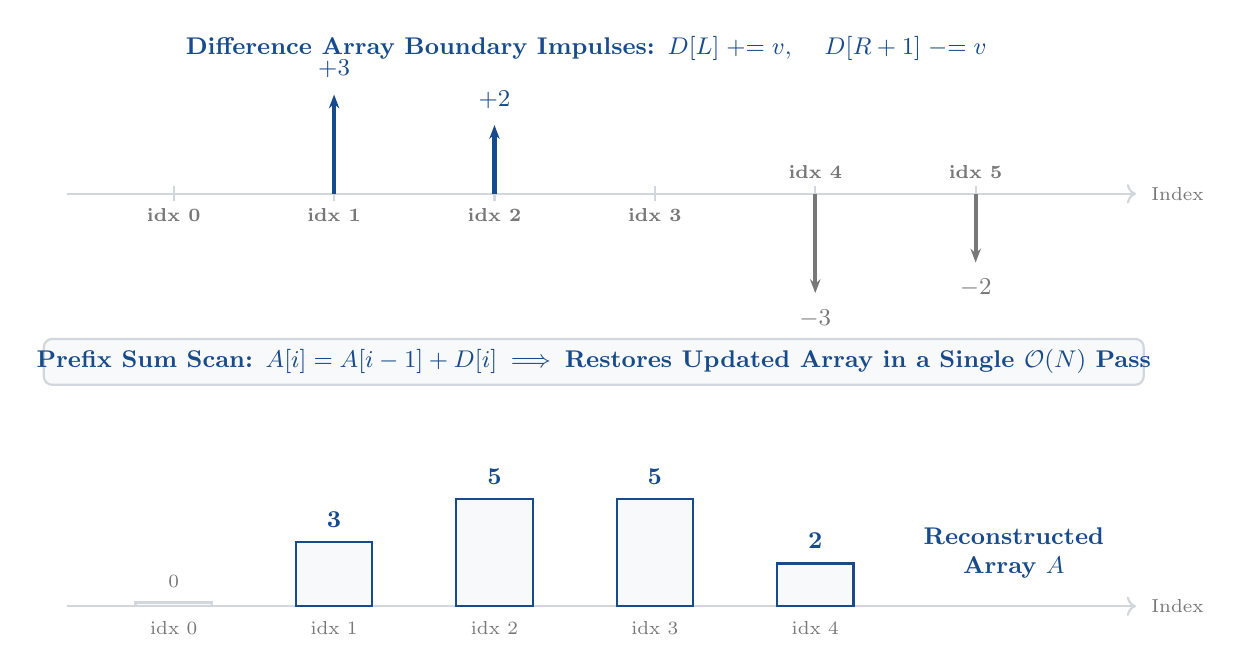
\begin{tikzpicture}[scale=0.97, every node/.style={transform shape}]
    % Top Title Banner
    \node[font=\small\bfseries, primaryblue] at (7.6, 6.7) {Difference Array Boundary Impulses: $D[L] \mathrel{+}= v, \quad D[R+1] \mathrel{-}= v$};

    % Axis for D (x from 0.8 to 14.8 at y = 4.8)
    \draw[->, thick, draw=codeframe] (0.8, 4.8) -- (14.8, 4.8) node[right=2pt, font=\scriptsize, codegray] {Index};

    % Ticks & Index numbers placed cleanly on the opposite side of each impulse to prevent line crossing!
    \foreach \i/\pos/\txt in {0/below/0, 1/below/1, 2/below/2, 3/below/3, 4/above/4, 5/above/5} {
        \pgfmathsetmacro{\xpos}{2.2 + \i * 2.1}
        \draw[thick, draw=codeframe] (\xpos, 4.7) -- (\xpos, 4.9);
        \node[font=\scriptsize\bfseries, codegray, \pos=2pt] at (\xpos, 4.8) {idx \txt};
    }

    % Upward Impulses (positive increments)
    % idx 1: +3 (from y=4.8 up to 6.1)
    \draw[->, line width=1.5pt, primaryblue, -{Stealth[length=5pt]}] (4.3, 4.8) -- (4.3, 6.1)
        node[above=2pt, font=\small\bfseries, primaryblue] {$+3$};
    % idx 2: +2 (from y=4.8 up to 5.7)
    \draw[->, line width=1.5pt, primaryblue, -{Stealth[length=5pt]}] (6.4, 4.8) -- (6.4, 5.7)
        node[above=2pt, font=\small\bfseries, primaryblue] {$+2$};

    % Downward Impulses (negative boundary cancels)
    % idx 4: -3 (from y=4.8 down to 3.5)
    \draw[->, line width=1.5pt, codegray, -{Stealth[length=5pt]}] (10.6, 4.8) -- (10.6, 3.5)
        node[below=2pt, font=\small\bfseries, codegray] {$-3$};
    % idx 5: -2 (from y=4.8 down to 3.9)
    \draw[->, line width=1.5pt, codegray, -{Stealth[length=5pt]}] (12.7, 4.8) -- (12.7, 3.9)
        node[below=2pt, font=\small\bfseries, codegray] {$-2$};

    % Middle Transition Banner across full textwidth
    \draw[draw=codeframe, fill=codebg, rounded corners=3pt, thick] (0.5, 2.3) rectangle (14.9, 2.9);
    \node[font=\small\bfseries, primaryblue] at (7.7, 2.6) {
        Prefix Sum Scan: $A[i] = A[i-1] + D[i] \implies \text{Restores Updated Array in a Single } \mathcal{O}(N) \text{ Pass}$
    };

    % Bottom: Reconstructed Array Bar Chart (y baseline at -0.6)
    \begin{scope}[yshift=-0.6cm]
        \draw[->, thick, draw=codeframe] (0.8, 0) -- (14.8, 0) node[right=2pt, font=\scriptsize, codegray] {Index};

        % Bars: [0, 3, 5, 5, 2] with scaled heights (max height = 1.4cm for value 5)
        % idx 0: 0
        \draw[fill=codebg, draw=codeframe, thick] (1.7, 0) rectangle (2.7, 0.05);
        \node[above=2pt, font=\scriptsize, codegray] at (2.2, 0.05) {0};
        \node[below=2pt, font=\scriptsize, codegray] at (2.2, 0) {idx 0};

        % idx 1: 3 (height 0.84)
        \draw[fill=codebg, draw=primaryblue, thick] (3.8, 0) rectangle (4.8, 0.84);
        \node[above=2pt, font=\small\bfseries, primaryblue] at (4.3, 0.84) {3};
        \node[below=2pt, font=\scriptsize, codegray] at (4.3, 0) {idx 1};

        % idx 2: 5 (height 1.4)
        \draw[fill=codebg, draw=primaryblue, thick] (5.9, 0) rectangle (6.9, 1.4);
        \node[above=2pt, font=\small\bfseries, primaryblue] at (6.4, 1.4) {5};
        \node[below=2pt, font=\scriptsize, codegray] at (6.4, 0) {idx 2};

        % idx 3: 5 (height 1.4)
        \draw[fill=codebg, draw=primaryblue, thick] (8.0, 0) rectangle (9.0, 1.4);
        \node[above=2pt, font=\small\bfseries, primaryblue] at (8.5, 1.4) {5};
        \node[below=2pt, font=\scriptsize, codegray] at (8.5, 0) {idx 3};

        % idx 4: 2 (height 0.56)
        \draw[fill=codebg, draw=primaryblue, thick] (10.1, 0) rectangle (11.1, 0.56);
        \node[above=2pt, font=\small\bfseries, primaryblue] at (10.6, 0.56) {2};
        \node[below=2pt, font=\scriptsize, codegray] at (10.6, 0) {idx 4};

        \node[font=\bfseries\small, primaryblue, align=center] at (13.2, 0.7) {Reconstructed\\Array $A$};
    \end{scope}
\end{tikzpicture}
\caption{Difference array impulse spikes and prefix integration. Each range addition injects two boundary markers in $O(1)$. A final cumulative sweep reconstructs the flat step-function intervals.}
\end{figure}

\newpage
% ============================================================================
\section{Module 05: Recursion and Backtracking}
% ============================================================================

\subsection{Diagram 10: Call Stack Activation Frames Lifecycle}

\breadcrumb{05.recursion_and_backtracking.tex}{Section 1.1: Call Stacks}{Mechanically demonstrates stack frame allocation during recursive descent and subsequent deallocation during the unwinding return phase for \texttt{fac(4)}.}

\diagramaudit{Agent (Antigravity)}{2026-10-11}{Structured into 3 clear horizontal phases: recursive descent (stack growth), horizontal base-case return transition, and unwinding ascent (frame popping); added evaluation cascade card tracking factorial computations ($1 \to 2 \to 6 \to 24$) and $O(N)$ stack space invariant.}

\begin{figure}[htbp]
\centering
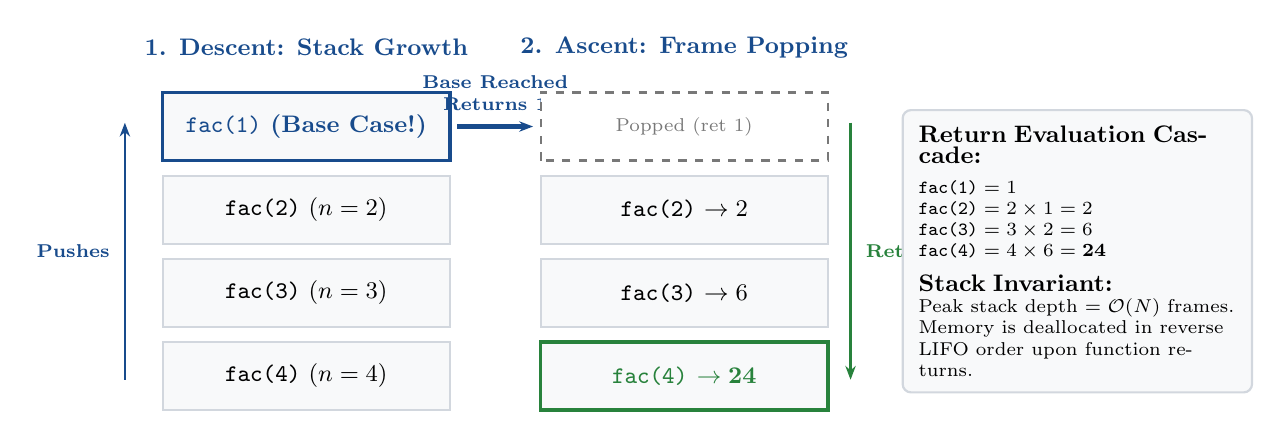
\begin{tikzpicture}[scale=0.96, every node/.style={transform shape}]
    % Col 1: Descent (Pushing) x in 0.8 to 4.6
    \node[font=\small\bfseries, primaryblue] at (2.7, 5.0) {1. Descent: Stack Growth};

    \draw[->, thick, primaryblue, -{Stealth[length=5pt]}] (0.3, 0.6) -- (0.3, 4.0)
        node[midway, left=2pt, font=\scriptsize\bfseries, primaryblue] {Pushes};

    \draw[thick, draw=codeframe, fill=codebg] (0.8, 0.2) rectangle (4.6, 1.1)
        node[midway, font=\small] {\texttt{fac(4)} ($n=4$)};
    \draw[thick, draw=codeframe, fill=codebg] (0.8, 1.3) rectangle (4.6, 2.2)
        node[midway, font=\small] {\texttt{fac(3)} ($n=3$)};
    \draw[thick, draw=codeframe, fill=codebg] (0.8, 2.4) rectangle (4.6, 3.3)
        node[midway, font=\small] {\texttt{fac(2)} ($n=2$)};
    \draw[line width=1.3pt, draw=primaryblue, fill=codebg] (0.8, 3.5) rectangle (4.6, 4.4)
        node[midway, font=\small\bfseries, primaryblue] {\texttt{fac(1)} (Base Case!)};

    % Transition Arrow at the top between base case and unwinding
    \draw[->, line width=1.6pt, primaryblue, -{Stealth[length=5pt]}] (4.7, 3.95) -- (5.7, 3.95)
        node[midway, above=2pt, font=\scriptsize\bfseries, align=center, text=primaryblue] {Base Reached\\Returns 1};

    % Col 2: Ascent (Unwinding) x in 5.8 to 9.6
    \node[font=\small\bfseries, primaryblue] at (7.7, 5.0) {2. Ascent: Frame Popping};

    \draw[line width=1.3pt, draw=codegreen, fill=codebg] (5.8, 0.2) rectangle (9.6, 1.1)
        node[midway, font=\small\bfseries, codegreen] {\texttt{fac(4)} $\to \mathbf{24}$};
    \draw[thick, draw=codeframe, fill=codebg] (5.8, 1.3) rectangle (9.6, 2.2)
        node[midway, font=\small] {\texttt{fac(3)} $\to 6$};
    \draw[thick, draw=codeframe, fill=codebg] (5.8, 2.4) rectangle (9.6, 3.3)
        node[midway, font=\small] {\texttt{fac(2)} $\to 2$};
    \draw[thick, dashed, draw=codegray, fill=white] (5.8, 3.5) rectangle (9.6, 4.4)
        node[midway, font=\scriptsize, codegray] {Popped (ret 1)};

    \draw[->, thick, codegreen, -{Stealth[length=5pt]}] (9.9, 4.0) -- (9.9, 0.6)
        node[midway, right=2pt, font=\scriptsize\bfseries, codegreen] {Returns};

    % Col 3: Calculation & Space Complexity Card (x in 10.6 to 15.2)
    \node[draw=codeframe, fill=codebg, rounded corners=3pt, thick, align=left, font=\scriptsize, inner sep=6pt, text width=4.2cm] at (12.9, 2.3) {
        \textbf{\small Return Evaluation Cascade:}\\[3pt]
        $\texttt{fac(1)} = 1$\\
        $\texttt{fac(2)} = 2 \times 1 = 2$\\
        $\texttt{fac(3)} = 3 \times 2 = 6$\\
        $\texttt{fac(4)} = 4 \times 6 = \mathbf{24}$\\[5pt]
        \textbf{\small Stack Invariant:}\\
        Peak stack depth $= \mathcal{O}(N)$ frames. Memory is deallocated in reverse LIFO order upon function returns.
    };
\end{tikzpicture}
\caption{Call stack activation frames lifecycle for recursive factorial. Each recursive call allocates a local frame; reaching the base case triggers the return cascade and frame deallocation.}
\end{figure}

\newpage
\subsection{Diagram 11: Fibonacci Recursion Tree with Redundant Subproblems}

\breadcrumb{05.recursion_and_backtracking.tex}{Section 1.2: Recursion Tree (replaces missing tree at line 131)}{Renders the promised recursion tree for $\text{fib}(4)$, explicitly boxing identical subtrees to demonstrate the exponential $O(2^n)$ duplication that motivates DP.}

\diagramaudit{Agent (Antigravity)}{2026-10-11}{Replaced broken placeholder at line 131; widened tree node layout across $14.8\text{ cm}$ to eliminate node collisions; highlighted duplicate $\texttt{fib(2)}$ subtrees in dashed boxes with non-colliding labels; added memoization bottom card detailing exponential $O(2^n)$ duplication collapse into $O(n)$ chain.}

\begin{figure}[htbp]
\centering
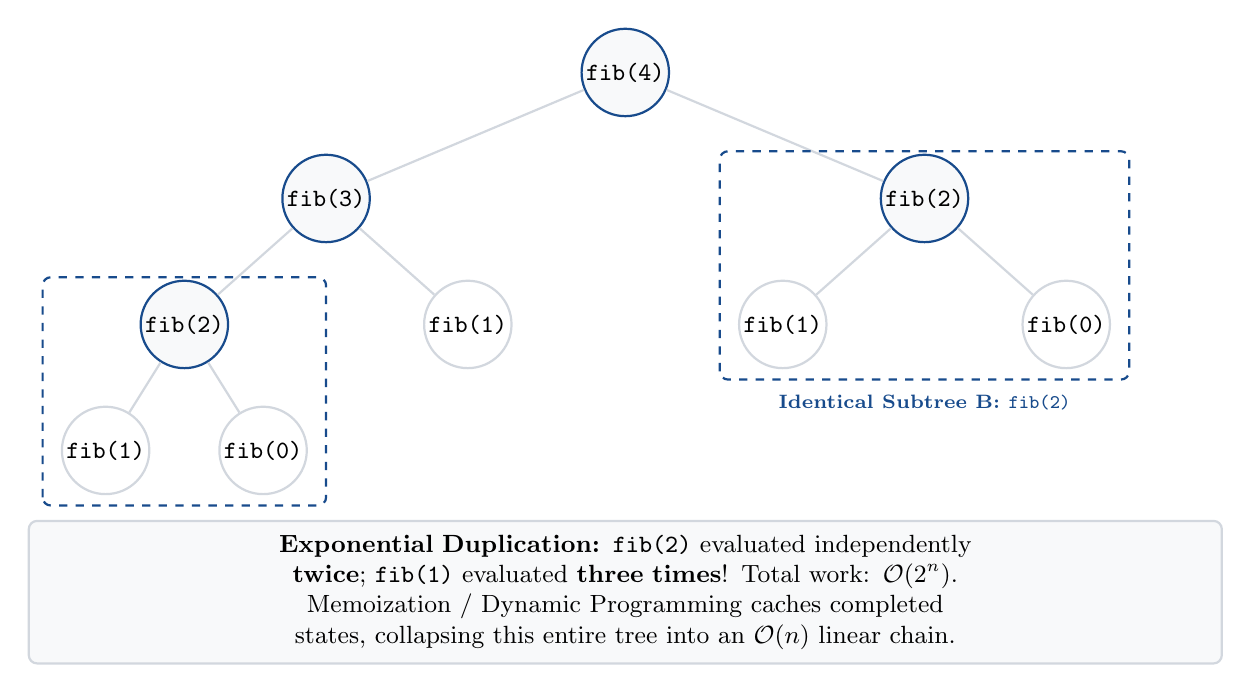
\begin{tikzpicture}[
    fibnode/.style={circle, draw=primaryblue, fill=codebg, thick, font=\small\bfseries, inner sep=1pt, minimum size=1.05cm},
    basenode/.style={circle, draw=codeframe, fill=white, thick, font=\small, inner sep=1pt, minimum size=1.05cm}
]
    % Root fib(4)
    \node[fibnode] (r) at (7.6, 5.0) {\texttt{fib(4)}};

    % Level 1
    \node[fibnode] (f3) at (3.8, 3.4) {\texttt{fib(3)}};
    \node[fibnode] (f2_r) at (11.4, 3.4) {\texttt{fib(2)}};
    \draw[thick, draw=codeframe] (r) -- (f3);
    \draw[thick, draw=codeframe] (r) -- (f2_r);

    % Level 2
    \node[fibnode] (f2_l) at (2.0, 1.8) {\texttt{fib(2)}};
    \node[basenode] (f1_m) at (5.6, 1.8) {\texttt{fib(1)}};
    \draw[thick, draw=codeframe] (f3) -- (f2_l);
    \draw[thick, draw=codeframe] (f3) -- (f1_m);

    \node[basenode] (f1_r) at (9.6, 1.8) {\texttt{fib(1)}};
    \node[basenode] (f0_r) at (13.2, 1.8) {\texttt{fib(0)}};
    \draw[thick, draw=codeframe] (f2_r) -- (f1_r);
    \draw[thick, draw=codeframe] (f2_r) -- (f0_r);

    % Level 3
    \node[basenode] (f1_l) at (1.0, 0.2) {\texttt{fib(1)}};
    \node[basenode] (f0_l) at (3.0, 0.2) {\texttt{fib(0)}};
    \draw[thick, draw=codeframe] (f2_l) -- (f1_l);
    \draw[thick, draw=codeframe] (f2_l) -- (f0_l);

    % Highlight duplicate subtrees
    \draw[thick, draw=primaryblue, dashed, rounded corners=3pt] (0.2, -0.5) rectangle (3.8, 2.4);
    \node[primaryblue, font=\scriptsize\bfseries, below=2pt] at (2.0, -0.5) {Subtree A: \texttt{fib(2)}};

    \draw[thick, draw=primaryblue, dashed, rounded corners=3pt] (8.8, 1.1) rectangle (14.0, 4.0);
    \node[primaryblue, font=\scriptsize\bfseries, below=2pt] at (11.4, 1.1) {Identical Subtree B: \texttt{fib(2)}};

    % Bottom card across full width
    \node[draw=codeframe, fill=codebg, rounded corners=3pt, thick, align=center, font=\small, inner sep=5pt, text width=14.8cm] at (7.6, -1.6) {
        \textbf{Exponential Duplication:} \texttt{fib(2)} evaluated independently \textbf{twice}; \texttt{fib(1)} evaluated \textbf{three times}! Total work: $\mathcal{O}(2^n)$.\\
        Memoization / Dynamic Programming caches completed states, collapsing this entire tree into an $\mathcal{O}(n)$ linear chain.
    };
\end{tikzpicture}
\caption{Fibonacci recursion tree for $\text{fib}(4)$. Duplicate subtrees (highlighted in dashed boxes) recompute identical subproblems, proving the exponential runtime of unmemoized recursion.}
\end{figure}

\newpage
\subsection{Diagram 12: Backtracking Decision Tree with Rollback and Pruning}

\breadcrumb{05.recursion_and_backtracking.tex}{Section 2.1: Generate Parentheses (replaces missing tree at lines 282 \& 294)}{Visualizes state exploration, early branch pruning ($\times$), and rollback restoration for Generate Parentheses with $n=2$.}

\diagramaudit{Agent (Antigravity)}{2026-10-11}{Replaced broken placeholders at lines 282 \& 294 for Generate Parentheses ($n=2$); rendered pruned branches with dashed borders and explicit cutoff conditions; spaced valid leaf nodes with $0.6\text{ cm}$ vertical clearance; added right panel explaining feasibility invariants, pruning, and state rollback.}

\begin{figure}[htbp]
\centering
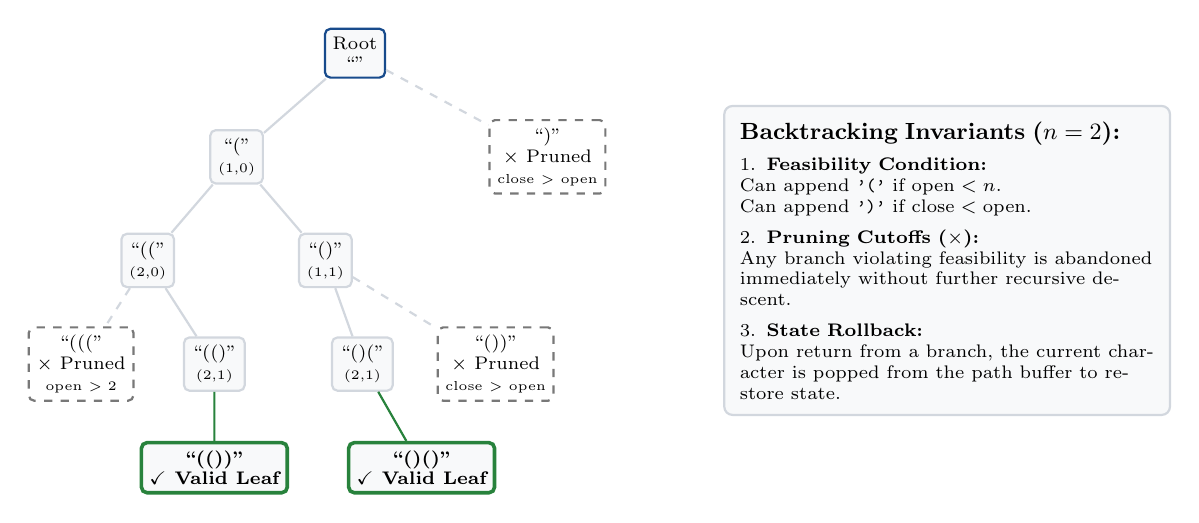
\begin{tikzpicture}[
    scale=0.94, every node/.style={transform shape},
    tree_node/.style={rectangle, rounded corners=2pt, draw=codeframe, fill=codebg, thick, font=\scriptsize, align=center, inner sep=3pt},
    pruned_node/.style={rectangle, rounded corners=2pt, draw=codegray, dashed, fill=white, thick, font=\scriptsize, align=center, inner sep=3pt},
    leaf_node/.style={rectangle, rounded corners=2pt, draw=codegreen, fill=codebg, line width=1.3pt, font=\scriptsize\bfseries, align=center, inner sep=3pt}
]
    % Root at (4.2, 5.0)
    \node[tree_node, draw=primaryblue] (root) at (4.2, 5.0) {Root\\``''};

    % Level 1
    \node[tree_node] (n_open) at (2.6, 3.6) {``(''\\{\tiny (1,0)}};
    \node[pruned_node] (n_close_pruned) at (6.8, 3.6) {``)''\\$\times$ Pruned\\{\tiny close $>$ open}};
    \draw[thick, draw=codeframe] (root) -- (n_open);
    \draw[thick, draw=codeframe, dashed] (root) -- (n_close_pruned);

    % Level 2 (under n_open)
    \node[tree_node] (n_oo) at (1.4, 2.2) {``((''\\{\tiny (2,0)}};
    \node[tree_node] (n_oc) at (3.8, 2.2) {``()''\\{\tiny (1,1)}};
    \draw[thick, draw=codeframe] (n_open) -- (n_oo);
    \draw[thick, draw=codeframe] (n_open) -- (n_oc);

    % Level 3
    \node[pruned_node] (n_ooo_pruned) at (0.5, 0.8) {``(((''\\$\times$ Pruned\\{\tiny open $>2$}};
    \node[tree_node] (n_ooc) at (2.3, 0.8) {``(()''\\{\tiny (2,1)}};
    \draw[thick, draw=codeframe, dashed] (n_oo) -- (n_ooo_pruned);
    \draw[thick, draw=codeframe] (n_oo) -- (n_ooc);

    \node[tree_node] (n_oco) at (4.3, 0.8) {``()(''\\{\tiny (2,1)}};
    \node[pruned_node] (n_occ_pruned) at (6.1, 0.8) {``())''\\$\times$ Pruned\\{\tiny close $>$ open}};
    \draw[thick, draw=codeframe] (n_oc) -- (n_oco);
    \draw[thick, draw=codeframe, dashed] (n_oc) -- (n_occ_pruned);

    % Level 4 (leaves spaced out with 0.6cm clearance)
    \node[leaf_node] (leaf1) at (2.3, -0.6) {``(())''\\$\checkmark$ Valid Leaf};
    \node[leaf_node] (leaf2) at (5.1, -0.6) {``()()''\\$\checkmark$ Valid Leaf};
    \draw[thick, draw=codegreen] (n_ooc) -- (leaf1);
    \draw[thick, draw=codegreen] (n_oco) -- (leaf2);

    % Right Side Panel: Backtracking Invariants Card (x in 9.2 to 15.2)
    \node[draw=codeframe, fill=codebg, rounded corners=3pt, thick, align=left, font=\scriptsize, inner sep=6pt, text width=5.6cm] at (12.2, 2.2) {
        \textbf{\small Backtracking Invariants ($n=2$):}\\[4pt]
        1. \textbf{Feasibility Condition:}\\
        Can append \texttt{'('} if $\text{open} < n$.\\
        Can append \texttt{')'} if $\text{close} < \text{open}$.\\[4pt]
        2. \textbf{Pruning Cutoffs ($\times$):}\\
        Any branch violating feasibility is abandoned immediately without further recursive descent.\\[4pt]
        3. \textbf{State Rollback:}\\
        Upon return from a branch, the current character is popped from the path buffer to restore state.
    };
\end{tikzpicture}
\caption{Backtracking decision tree for Generate Parentheses ($n=2$). Dashed nodes represent pruned paths aborted immediately upon violating feasibility invariants.}
\end{figure}

\newpage
% ============================================================================
\section{Module 06: Dynamic Programming}
% ============================================================================

\subsection{Diagram 13: 1D DP State Dependency Tape}

\breadcrumb{06.dynamic_programming.tex}{Section 2.1: 1D DP (House Robber)}{Illustrates state transitions $dp[i] = \max(dp[i-1], dp[i-2] + \text{val})$ and the sliding window space optimization reducing $O(N)$ space to $O(1)$.}

\diagramaudit{Agent (Antigravity)}{2026-10-11}{Aligned house values $A[i]$ directly above DP state tape $dp[i]$; highlighted actively evaluated cell $dp[2]$; drew skip transition ($dp[1] \to dp[2]$) and rob curved arc ($dp[0] + A[2] \to dp[2]$); added full-width sliding window space optimization card demonstrating 2-variable rolling state ($O(N) \to O(1)$).}

\begin{figure}[htbp]
\centering
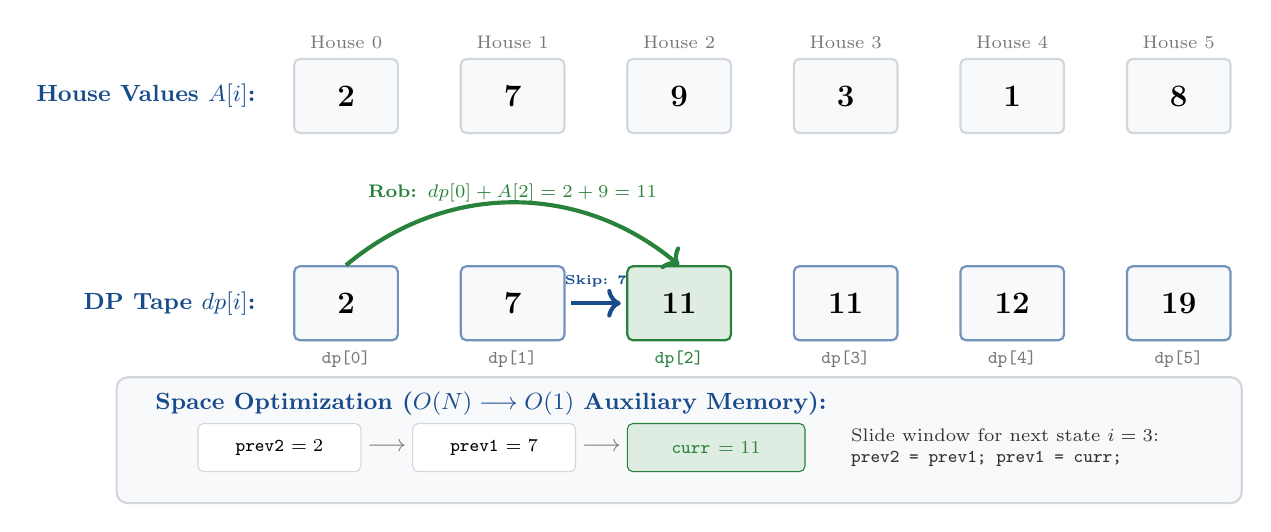
\begin{tikzpicture}[
    scale=0.94, every node/.style={transform shape},
    cell/.style={draw=codeframe, fill=white, thick, rounded corners=2pt, minimum width=1.4cm, minimum height=1.0cm, align=center},
    housecell/.style={draw=codeframe, fill=codebg, thick, rounded corners=2pt, minimum width=1.4cm, minimum height=1.0cm, align=center},
    dpcell/.style={draw=primaryblue!60, fill=codebg, thick, rounded corners=2pt, minimum width=1.4cm, minimum height=1.0cm, align=center},
    activecell/.style={draw=codegreen, fill=codegreen!15, thick, rounded corners=2pt, minimum width=1.4cm, minimum height=1.0cm, align=center}
]
    % Left row labels
    \node[anchor=east, font=\bfseries\small, text=primaryblue] at (2.0, 5.2) {House Values $A[i]$:};
    \node[anchor=east, font=\bfseries\small, text=primaryblue] at (2.0, 2.4) {DP Tape $dp[i]$:};

    % 6 Houses (indices 0..5) at y = 5.2
    \foreach \i/\val in {0/2, 1/7, 2/9, 3/3, 4/1, 5/8} {
        \pgfmathsetmacro{\cx}{3.1 + \i * 2.25}
        \node[housecell] (H\i) at (\cx, 5.2) {\textbf{\large \val}};
        \node[above, font=\scriptsize, text=codegray] at (H\i.north) {House $\i$};
    }

    % DP Cells (indices 0..5) at y = 2.4
    \foreach \i/\val in {0/2, 1/7, 3/11, 4/12, 5/19} {
        \pgfmathsetmacro{\cx}{3.1 + \i * 2.25}
        \node[dpcell] (DP\i) at (\cx, 2.4) {\textbf{\large \val}};
        \node[below, font=\scriptsize\ttfamily, text=codegray] at (DP\i.south) {dp[\i]};
    }
    % Highlight DP2 being computed
    \node[activecell] (DP2) at (7.6, 2.4) {\textbf{\large 11}};
    \node[below, font=\scriptsize\ttfamily\bfseries, text=codegreen] at (DP2.south) {dp[2]};

    % Transition arrows for dp[2]
    % Skip: dp[1] -> dp[2]
    \draw[->, line width=1.5pt, primaryblue, shorten <= 2pt, shorten >= 2pt] (DP1.east) -- (DP2.west)
        node[midway, above=2pt, font=\tiny\bfseries, text=primaryblue] {Skip: 7};

    % Rob: dp[0] + House[2] -> dp[2]
    \draw[->, line width=1.5pt, codegreen] (DP0.north) to[out=40, in=140] (DP2.north);
    \node[above, font=\scriptsize\bfseries, text=codegreen] at (5.35, 3.65) {Rob: $dp[0] + A[2] = 2 + 9 = 11$};

    % Sliding window space optimization card spanning full width
    \draw[draw=codeframe, fill=codebg, rounded corners=4pt, thick] (0.0, -0.3) rectangle (15.2, 1.4);

    % Inside sliding window card
    \node[anchor=west, font=\bfseries\small, text=primaryblue] at (0.4, 1.05) {Space Optimization ($O(N) \longrightarrow O(1)$ Auxiliary Memory):};
    
    % Register boxes
    \node[draw=codeframe, fill=white, rounded corners=2pt, minimum width=2.2cm, minimum height=0.65cm, font=\scriptsize] at (2.2, 0.45) {\texttt{prev2} $= 2$};
    \node[font=\small, text=codegray] at (3.65, 0.45) {$\longrightarrow$};
    \node[draw=codeframe, fill=white, rounded corners=2pt, minimum width=2.2cm, minimum height=0.65cm, font=\scriptsize] at (5.1, 0.45) {\texttt{prev1} $= 7$};
    \node[font=\small, text=codegray] at (6.55, 0.45) {$\longrightarrow$};
    \node[draw=codegreen, fill=codegreen!15, rounded corners=2pt, minimum width=2.4cm, minimum height=0.65cm, font=\scriptsize\bfseries, text=codegreen] at (8.1, 0.45) {\texttt{curr} $= 11$};

    \node[anchor=west, font=\scriptsize, text=black!80, align=left] at (9.8, 0.45) {
        Slide window for next state $i=3$:\\
        \texttt{prev2 = prev1; prev1 = curr;}
    };
\end{tikzpicture}
\caption{1D DP state dependency tape for House Robber ($N=6$). Computing cell $dp[i]$ references strictly $dp[i-1]$ and $dp[i-2]$, enabling rolling two-variable window optimization from $O(N)$ down to $O(1)$ auxiliary space.}
\end{figure}

\newpage
\subsection{Diagram 14: 2D Grid DP Path Transition Matrix}

\breadcrumb{06.dynamic_programming.tex}{Section 2.2: 2D DP on Grids (Minimum Path Sum)}{Illustrates grid path planning where state cell $dp[i][j]$ aggregates optimal sub-paths arriving strictly from the top and left neighboring cells.}

\diagramaudit{Agent (Antigravity)}{2026-10-11}{Formatted $3 \times 3$ grid displaying cell coordinates, step costs, and accumulated DP values; highlighted global minimum path with thick green arrows; visualized dual predecessor transitions (Left vs Top) for cell $(1,1)$; added right panel with recurrence formula, arithmetic trace, and rolling vector space optimization.}

\begin{figure}[htbp]
\centering
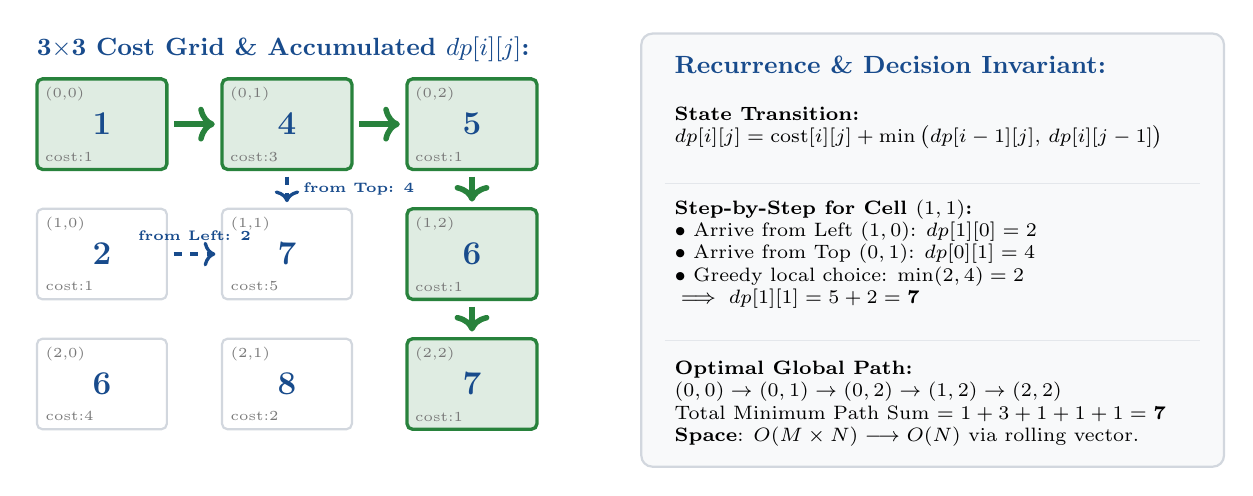
\begin{tikzpicture}[
    gridcell/.style={draw=codeframe, fill=white, thick, rounded corners=2pt, minimum width=1.65cm, minimum height=1.15cm, align=center},
    pathcell/.style={draw=codegreen, fill=codegreen!15, line width=1.2pt, rounded corners=2pt, minimum width=1.65cm, minimum height=1.15cm, align=center}
]
    % --- Left Panel: 3x3 Grid ---
    \node[anchor=west, font=\bfseries\small, text=primaryblue] at (0.0, 5.7) {3$\times$3 Cost Grid \& Accumulated $dp[i][j]$:};

    % Draw 3x3 cells
    % Costs:
    % (0,0)=1, (0,1)=3, (0,2)=1
    % (1,0)=1, (1,1)=5, (1,2)=1
    % (2,0)=4, (2,1)=2, (2,2)=1
    % DP:
    % (0,0)=1, (0,1)=4, (0,2)=5
    % (1,0)=2, (1,1)=7, (1,2)=6
    % (2,0)=6, (2,1)=8, (2,2)=7
    
    % Optimal path: (0,0)->(0,1)->(0,2)->(1,2)->(2,2)
    \foreach \r/\c/\cost/\dpval/\ispath in {
        0/0/1/1/1, 0/1/3/4/1, 0/2/1/5/1,
        1/0/1/2/0, 1/1/5/7/0, 1/2/1/6/1,
        2/0/4/6/0, 2/1/2/8/0, 2/2/1/7/1
    } {
        \pgfmathsetmacro{\cx}{0.95 + \c * 2.35}
        \pgfmathsetmacro{\cy}{4.75 - \r * 1.65}
        \ifnum\ispath=1
            \node[pathcell] (C\r\c) at (\cx, \cy) {};
        \else
            \node[gridcell] (C\r\c) at (\cx, \cy) {};
        \fi
        \node[font=\tiny, text=codegray, anchor=north west] at (C\r\c.north west) {(\r,\c)};
        \node[font=\tiny, text=codegray, anchor=south west] at (C\r\c.south west) {cost:\cost};
        \node[font=\large\bfseries, text=primaryblue, anchor=center] at (C\r\c.center) {\dpval};
    }

    % Optimal path arrows
    \draw[->, line width=2pt, codegreen, shorten <= 2pt, shorten >= 2pt] (C00.east) -- (C01.west);
    \draw[->, line width=2pt, codegreen, shorten <= 2pt, shorten >= 2pt] (C01.east) -- (C02.west);
    \draw[->, line width=2pt, codegreen, shorten <= 2pt, shorten >= 2pt] (C02.south) -- (C12.north);
    \draw[->, line width=2pt, codegreen, shorten <= 2pt, shorten >= 2pt] (C12.south) -- (C22.north);

    % Transition arrows for cell (1,1)
    \draw[->, line width=1.2pt, primaryblue, dashed, shorten <= 2pt, shorten >= 2pt] (C10.east) -- (C11.west)
        node[midway, above=1pt, font=\tiny\bfseries, text=primaryblue] {from Left: 2};
    \draw[->, line width=1.2pt, primaryblue, dashed, shorten <= 2pt, shorten >= 2pt] (C01.south) -- (C11.north)
        node[midway, right=2pt, font=\tiny\bfseries, text=primaryblue] {from Top: 4};

    % --- Right Panel: Computation Trace & Recurrence Card ---
    \draw[draw=codeframe, fill=codebg, rounded corners=4pt, thick] (7.8, 0.4) rectangle (15.2, 5.9);

    \node[anchor=west, font=\bfseries\small, text=primaryblue] at (8.1, 5.5) {Recurrence \& Decision Invariant:};

    \node[anchor=west, font=\scriptsize, align=left] at (8.1, 4.7) {
        \textbf{State Transition:}\\
        $dp[i][j] = \text{cost}[i][j] + \min\big(dp[i-1][j],\, dp[i][j-1]\big)$
    };

    \draw[draw=codeframe!60] (8.1, 4.0) -- (14.9, 4.0);

    \node[anchor=west, font=\scriptsize, align=left] at (8.1, 3.1) {
        \textbf{Step-by-Step for Cell $(1,1)$:}\\
        $\bullet$ Arrive from Left $(1,0)$: $dp[1][0] = 2$\\
        $\bullet$ Arrive from Top $(0,1)$: $dp[0][1] = 4$\\
        $\bullet$ Greedy local choice: $\min(2, 4) = 2$\\
        $\implies dp[1][1] = 5 + 2 = \mathbf{7}$
    };

    \draw[draw=codeframe!60] (8.1, 2.0) -- (14.9, 2.0);

    \node[anchor=west, font=\scriptsize, align=left] at (8.1, 1.2) {
        \textbf{Optimal Global Path:}\\
        $(0,0) \to (0,1) \to (0,2) \to (1,2) \to (2,2)$\\
        Total Minimum Path Sum $= 1 + 3 + 1 + 1 + 1 = \mathbf{7}$\\
        \textbf{Space}: $O(M \times N) \longrightarrow O(N)$ via rolling vector.
    };
\end{tikzpicture}
\caption{2D Grid DP minimum path computation. Each cell evaluates strictly its top and left predecessor cells. The optimal path to the bottom-right terminal yields total cost 7.}
\end{figure}

\newpage
% ============================================================================
\section{Module 07: Graph Algorithms}
% ============================================================================

\subsection{Diagram 15: Graph Representation Comparison}

\breadcrumb{07.graph_algorithms.tex}{Section 2.4: Graph Representations in Code (replaces missing figure at lines 177--179)}{Fulfills the promised 4-node directed weighted graph and compares the spatial layout of an Adjacency Matrix against an Adjacency List side-by-side.}

\diagramaudit{Agent (Antigravity)}{2026-10-11}{Replaced broken placeholder at lines 177--179; designed 3 equal-width comparison cards across full page: 4-node directed weighted graph on left, $4 \times 4$ Adjacency Matrix in center, and Adjacency List on right; included time/space complexity trade-offs ($O(V^2)$ vs $O(V+E)$) on each card.}

\begin{figure}[htbp]
\centering
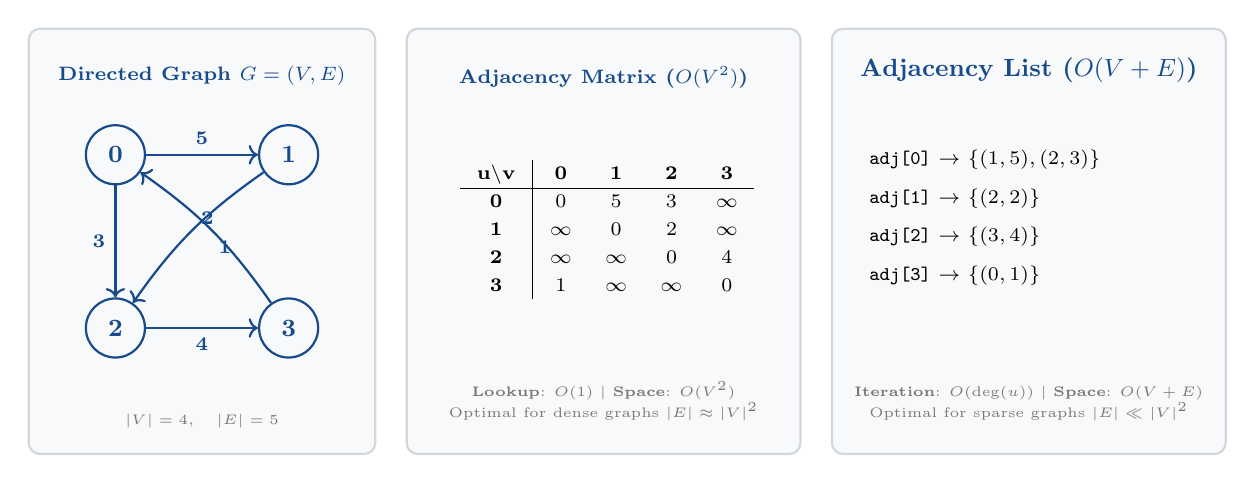
\begin{tikzpicture}[
    gnode/.style={circle, draw=primaryblue, fill=codebg, thick, minimum size=0.75cm, font=\bfseries\small, text=primaryblue},
    card/.style={draw=codeframe, fill=codebg, rounded corners=4pt, thick}
]
    % --- Column 1: Directed Weighted Graph (x: 0.0 to 4.4) ---
    \draw[card] (0.0, 0.0) rectangle (4.4, 5.4);
    \node[anchor=north, font=\bfseries\scriptsize, text=primaryblue] at (2.2, 5.05) {Directed Graph $G=(V,E)$};

    \node[gnode] (N0) at (1.1, 3.8) {0};
    \node[gnode] (N1) at (3.3, 3.8) {1};
    \node[gnode] (N2) at (1.1, 1.6) {2};
    \node[gnode] (N3) at (3.3, 1.6) {3};

    \draw[->, thick, primaryblue] (N0) -- (N1) node[midway, above, font=\scriptsize\bfseries] {5};
    \draw[->, thick, primaryblue] (N0) -- (N2) node[midway, left, font=\scriptsize\bfseries] {3};
    \draw[->, thick, primaryblue] (N1) to[out=-145, in=55] node[pos=0.25, below left, font=\scriptsize\bfseries] {2} (N2);
    \draw[->, thick, primaryblue] (N2) -- (N3) node[midway, below, font=\scriptsize\bfseries] {4};
    \draw[->, thick, primaryblue] (N3) to[out=125, in=-35] node[pos=0.25, above left, font=\scriptsize\bfseries] {1} (N0);

    \node[anchor=south, font=\tiny, text=codegray] at (2.2, 0.2) {$|V| = 4, \quad |E| = 5$};

    % --- Column 2: Adjacency Matrix (x: 4.8 to 9.8) ---
    \draw[card] (4.8, 0.0) rectangle (9.8, 5.4);
    \node[anchor=north, font=\bfseries\scriptsize, text=primaryblue] at (7.3, 5.05) {Adjacency Matrix ($O(V^2)$)};

    \node[anchor=center, font=\scriptsize] at (7.3, 2.85) {
        \renewcommand{\arraystretch}{1.25}
        \begin{tabular}{c|cccc}
        \textbf{u$\backslash$v} & \textbf{0} & \textbf{1} & \textbf{2} & \textbf{3} \\ \hline
        \textbf{0} & $0$ & $5$ & $3$ & $\infty$ \\
        \textbf{1} & $\infty$ & $0$ & $2$ & $\infty$ \\
        \textbf{2} & $\infty$ & $\infty$ & $0$ & $4$ \\
        \textbf{3} & $1$ & $\infty$ & $\infty$ & $0$ \\
        \end{tabular}
    };

    \node[anchor=south, font=\tiny, text=codegray, align=center] at (7.3, 0.3) {
        \textbf{Lookup}: $O(1)$ $\mid$ \textbf{Space}: $O(V^2)$\\
        Optimal for dense graphs $|E| \approx |V|^2$
    };

    % --- Column 3: Adjacency List (x: 10.2 to 15.2) ---
    \draw[card] (10.2, 0.0) rectangle (15.2, 5.4);
    \node[anchor=north, font=\bfseries\small, text=primaryblue] at (12.7, 5.15) {Adjacency List ($O(V+E)$)};

    \node[anchor=west, font=\scriptsize, align=left] at (10.55, 3.0) {
        \texttt{adj[0]} $\to$ $\{(1, 5), (2, 3)\}$\\[6pt]
        \texttt{adj[1]} $\to$ $\{(2, 2)\}$\\[6pt]
        \texttt{adj[2]} $\to$ $\{(3, 4)\}$\\[6pt]
        \texttt{adj[3]} $\to$ $\{(0, 1)\}$
    };

    \node[anchor=south, font=\tiny, text=codegray, align=center] at (12.7, 0.3) {
        \textbf{Iteration}: $O(\text{deg}(u))$ $\mid$ \textbf{Space}: $O(V+E)$\\
        Optimal for sparse graphs $|E| \ll |V|^2$
    };
\end{tikzpicture}
\caption{Visual comparison of a 4-node directed weighted graph alongside its Adjacency Matrix and Adjacency List representations across full text width.}
\end{figure}

\newpage
\subsection{Diagram 16: BFS Level Wavefront Expansion}

\breadcrumb{07.graph_algorithms.tex}{Section 3.1: Breadth-First Search (BFS)}{Demonstrates radial concentric ripple waves emanating from a source vertex, proving why BFS guarantees unweighted shortest paths.}

\diagramaudit{Agent (Antigravity)}{2026-10-11}{Drew concentric shaded circles representing radial distance wavefronts ($d=1, 2, 3$) with non-colliding labels in upper-left quadrant; routed tree edges from source $S$; added right panel tracking FIFO queue state progression across all levels and verified shortest path minimality invariant.}

\begin{figure}[htbp]
\centering
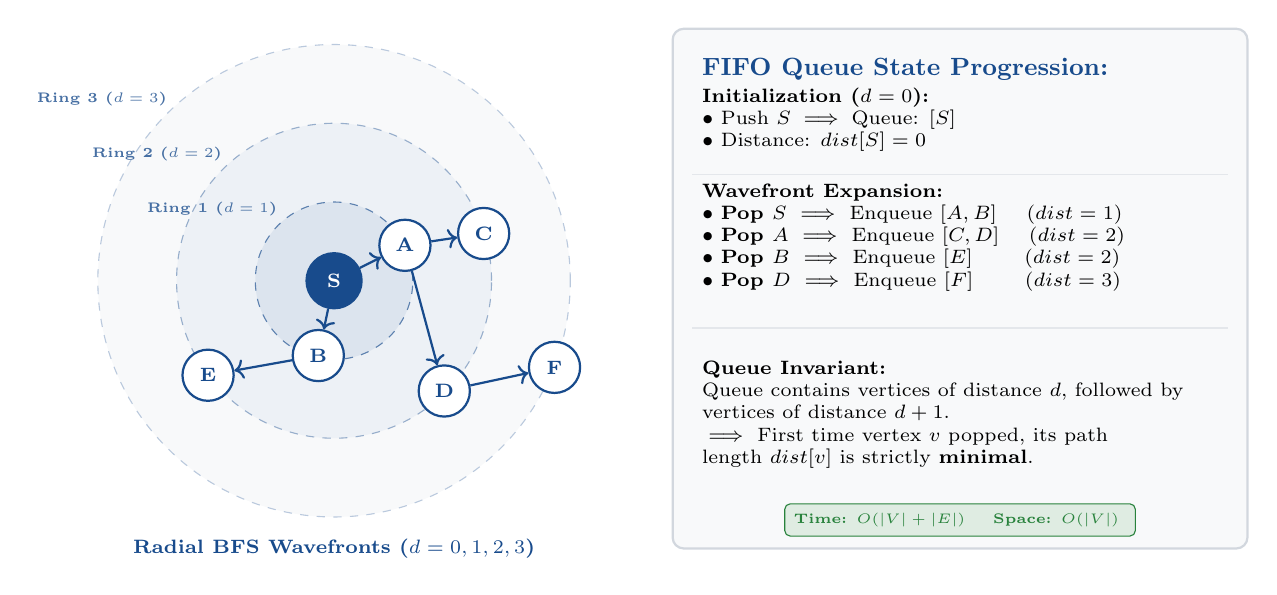
\begin{tikzpicture}[
    bnode/.style={circle, draw=primaryblue, fill=white, thick, minimum size=0.65cm, font=\bfseries\scriptsize, text=primaryblue},
    snode/.style={circle, draw=primaryblue, fill=primaryblue, thick, minimum size=0.7cm, font=\bfseries\scriptsize, text=white},
    card/.style={draw=codeframe, fill=codebg, rounded corners=4pt, thick}
]
    % --- Left Panel: BFS Concentric Wavefronts (x: 0.0 to 7.6) ---
    \begin{scope}[shift={(3.6, 3.1)}]
        % Concentric dashed rings
        \draw[fill=codebg, draw=primaryblue!30, dashed] (0, 0) circle (3.0);
        \draw[fill=primaryblue!8, draw=primaryblue!45, dashed] (0, 0) circle (2.0);
        \draw[fill=primaryblue!15, draw=primaryblue!70, dashed] (0, 0) circle (1.0);

        % Ring labels placed cleanly in upper-left quadrant
        \node[font=\tiny\bfseries, text=primaryblue!80, anchor=south east] at (-0.6, 0.7) {Ring 1 ($d=1$)};
        \node[font=\tiny\bfseries, text=primaryblue!80, anchor=south east] at (-1.3, 1.4) {Ring 2 ($d=2$)};
        \node[font=\tiny\bfseries, text=primaryblue!80, anchor=south east] at (-2.0, 2.1) {Ring 3 ($d=3$)};

        % Source Node S
        \node[snode] (S) at (0, 0) {S};

        % Level 1 Nodes
        \node[bnode] (A) at (0.9, 0.45) {A};
        \node[bnode] (B) at (-0.2, -0.95) {B};

        % Level 2 Nodes
        \node[bnode] (C) at (1.9, 0.6) {C};
        \node[bnode] (D) at (1.4, -1.4) {D};
        \node[bnode] (E) at (-1.6, -1.2) {E};

        % Level 3 Nodes
        \node[bnode] (F) at (2.8, -1.1) {F};

        % Tree Edges
        \draw[->, thick, primaryblue] (S) -- (A);
        \draw[->, thick, primaryblue] (S) -- (B);
        \draw[->, thick, primaryblue] (A) -- (C);
        \draw[->, thick, primaryblue] (A) -- (D);
        \draw[->, thick, primaryblue] (B) -- (E);
        \draw[->, thick, primaryblue] (D) -- (F);

        \node[anchor=north, font=\scriptsize\bfseries, text=primaryblue] at (0, -3.15) {Radial BFS Wavefronts ($d=0, 1, 2, 3$)};
    \end{scope}

    % --- Right Panel: FIFO Queue State Progression Card (x: 7.9 to 15.2) ---
    \draw[card] (7.9, -0.3) rectangle (15.2, 6.3);
    \node[anchor=north west, font=\bfseries\small, text=primaryblue] at (8.15, 6.05) {FIFO Queue State Progression:};

    \node[anchor=west, font=\scriptsize, align=left] at (8.15, 5.15) {
        \textbf{Initialization ($d=0$):}\\
        $\bullet$ Push $S \implies \text{Queue: } [S]$\\
        $\bullet$ Distance: $dist[S] = 0$
    };

    \draw[draw=codeframe!60] (8.15, 4.45) -- (14.95, 4.45);

    \node[anchor=west, font=\scriptsize, align=left] at (8.15, 3.65) {
        \textbf{Wavefront Expansion:}\\
        $\bullet$ \textbf{Pop $S$} $\implies$ Enqueue $[A, B]$ \quad ($dist = 1$)\\
        $\bullet$ \textbf{Pop $A$} $\implies$ Enqueue $[C, D]$ \quad ($dist = 2$)\\
        $\bullet$ \textbf{Pop $B$} $\implies$ Enqueue $[E]$ \quad\quad ($dist = 2$)\\
        $\bullet$ \textbf{Pop $D$} $\implies$ Enqueue $[F]$ \quad\quad ($dist = 3$)
    };

    \draw[draw=codeframe!60] (8.15, 2.5) -- (14.95, 2.5);

    \node[anchor=west, font=\scriptsize, align=left] at (8.15, 1.4) {
        \textbf{Queue Invariant:}\\
        Queue contains vertices of distance $d$, followed by\\
        vertices of distance $d+1$.\\
        $\implies$ First time vertex $v$ popped, its path\\
        length $dist[v]$ is strictly \textbf{minimal}.
    };

    \node[draw=codegreen, fill=codegreen!15, rounded corners=2pt, font=\tiny\bfseries, text=codegreen, anchor=south, align=center] at (11.55, -0.15) {
        Time: $O(|V| + |E|)$ \quad Space: $O(|V|)$
    };
\end{tikzpicture}
\caption{BFS wavefront expansion in concentric ripple layers across full text width. The FIFO queue processes all nodes at distance $d$ before any node at distance $d+1$, guaranteeing minimum edge paths.}
\end{figure}

\newpage
\subsection{Diagram 17: Dijkstra's Algorithm Priority Queue Edge Relaxation}

\breadcrumb{07.graph_algorithms.tex}{Section 3.5: Dijkstra's Algorithm}{Clarifies edge relaxation: how encountering a shorter candidate path via $u$ updates $dist[v]$ and enqueues the improved distance into the min-heap.}

\diagramaudit{Agent (Antigravity)}{2026-10-11}{Top panel illustrates source $S$, settled node $u$, and candidate node $v$; shows obsolete tentative path (weight 10) vs newly relaxed path ($4 + 3 = 7$); bottom panel splits into two cards explaining edge relaxation condition check and priority queue min-heap lazy deletion invariant.}

\begin{figure}[htbp]
\centering
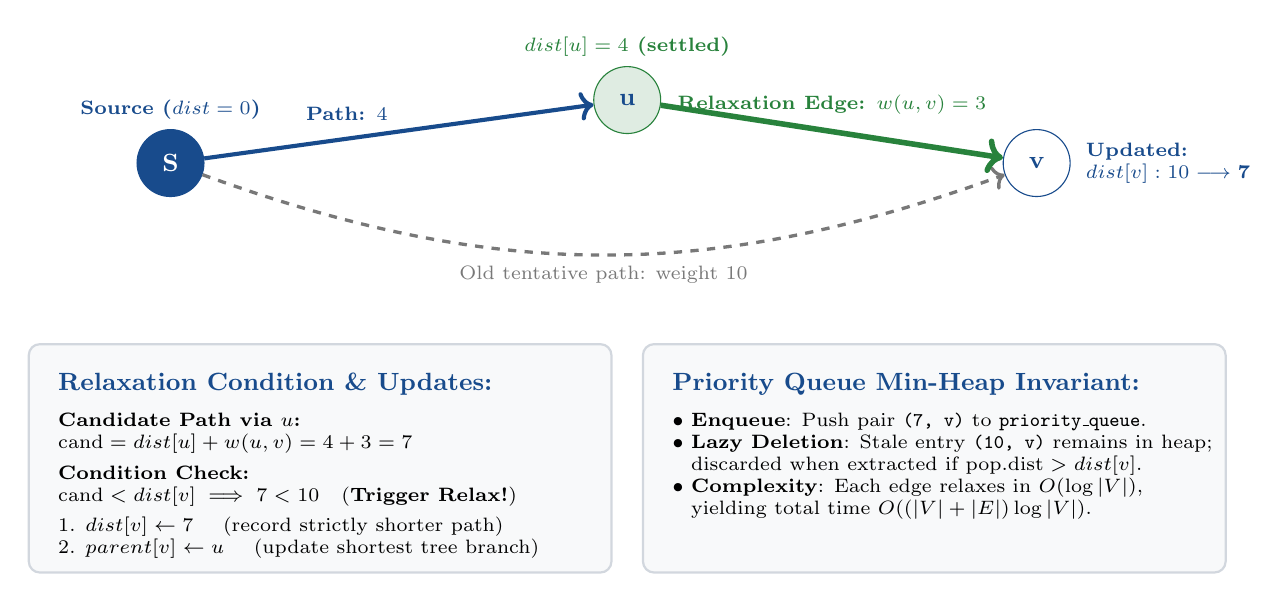
\begin{tikzpicture}[
    snode/.style={circle, draw=primaryblue, fill=primaryblue, text=white, font=\bfseries\small, minimum size=0.85cm},
    unode/.style={circle, draw=codegreen, fill=codegreen!15, text=primaryblue, font=\bfseries\small, minimum size=0.85cm},
    vnode/.style={circle, draw=primaryblue, fill=white, text=primaryblue, font=\bfseries\small, minimum size=0.85cm},
    card/.style={draw=codeframe, fill=codebg, rounded corners=4pt, thick}
]
    % --- Top Half: Graph Layout (Nodes S, u, v) ---
    \node[snode] (S) at (1.8, 5.0) {S};
    \node[above, font=\scriptsize\bfseries, text=primaryblue] at (S.north) {Source ($dist=0$)};

    \node[unode] (u) at (7.6, 5.8) {u};
    \node[above, font=\scriptsize\bfseries, text=codegreen] at (u.north) {$dist[u] = 4$ (settled)};

    \node[vnode] (v) at (12.8, 5.0) {v};
    \node[anchor=west, font=\scriptsize\bfseries, text=primaryblue, align=left, xshift=2pt] at (v.east) {Updated:\\$dist[v]: 10 \longrightarrow \mathbf{7}$};

    % Edge S -> u (settled path)
    \draw[->, line width=1.5pt, primaryblue] (S) -- (u)
        node[midway, above left, font=\scriptsize\bfseries, text=primaryblue] {Path: $4$};

    % Old suboptimal path S -> v (dashed curve)
    \draw[->, line width=1.2pt, codegray, dashed] (S) to[out=-20, in=-160]
        node[midway, below, font=\scriptsize, text=codegray] {Old tentative path: weight $10$} (v);

    % Relaxation edge u -> v
    \draw[->, line width=2pt, codegreen] (u) -- (v)
        node[midway, above, font=\scriptsize\bfseries, text=codegreen, yshift=2pt] {Relaxation Edge: $w(u,v) = 3$};

    % --- Bottom Half: Two Explanation Cards Spanning 15.2 cm ---
    % Card 1: Relaxation Condition
    \draw[card] (0.0, -0.2) rectangle (7.4, 2.7);
    \node[anchor=north west, font=\bfseries\small, text=primaryblue] at (0.25, 2.45) {Relaxation Condition \& Updates:};

    \node[anchor=north west, font=\scriptsize, align=left] at (0.25, 1.95) {
        \textbf{Candidate Path via $u$:}\\
        $\text{cand} = dist[u] + w(u,v) = 4 + 3 = 7$\\[3pt]
        \textbf{Condition Check:}\\
        $\text{cand} < dist[v] \implies 7 < 10 \quad \text{(\textbf{Trigger Relax!})}$\\[3pt]
        1. $dist[v] \leftarrow 7$ \quad (record strictly shorter path)\\
        2. $parent[v] \leftarrow u$ \quad (update shortest tree branch)
    };

    % Card 2: Min-Heap Queue Operation
    \draw[card] (7.8, -0.2) rectangle (15.2, 2.7);
    \node[anchor=north west, font=\bfseries\small, text=primaryblue] at (8.05, 2.45) {Priority Queue Min-Heap Invariant:};

    \node[anchor=north west, font=\scriptsize, align=left] at (8.05, 1.95) {
        $\bullet$ \textbf{Enqueue}: Push pair \texttt{(7, v)} to \texttt{priority\_queue}.\\
        $\bullet$ \textbf{Lazy Deletion}: Stale entry \texttt{(10, v)} remains in heap;\\
        \phantom{$\bullet$} discarded when extracted if $\text{pop.dist} > dist[v]$.\\
        $\bullet$ \textbf{Complexity}: Each edge relaxes in $O(\log |V|)$,\\
        \phantom{$\bullet$} yielding total time $O((|V| + |E|) \log |V|)$.
    };
\end{tikzpicture}
\caption{Dijkstra edge relaxation step across full text width. Finding a shorter path to $v$ through $u$ overwrites tentative distance $dist[v]$ from 10 to 7 and enqueues the improved pair into the min-heap.}
\end{figure}

\newpage
\subsection{Diagram 18: Disjoint Set Union (DSU) Path Compression}

\breadcrumb{07.graph_algorithms.tex}{Section 3.7: Minimum Spanning Tree and DSU}{Shows how recursive path compression flattens deep linear tree chains ($O(N)$) into depth-1 star graphs, achieving amortized $O(\alpha(N))$ operations.}

\diagramaudit{Agent (Antigravity)}{2026-10-11}{Structured into 3 columns: Before state showing degenerate chain of depth 4, center card showing recursive C++ implementation of \texttt{find(x)}, and After state showing flattened depth-1 star graph with calibrated angled arrows entering root 0 without overlapping; added $O(\alpha(N))$ complexity badge.}

\begin{figure}[htbp]
\centering
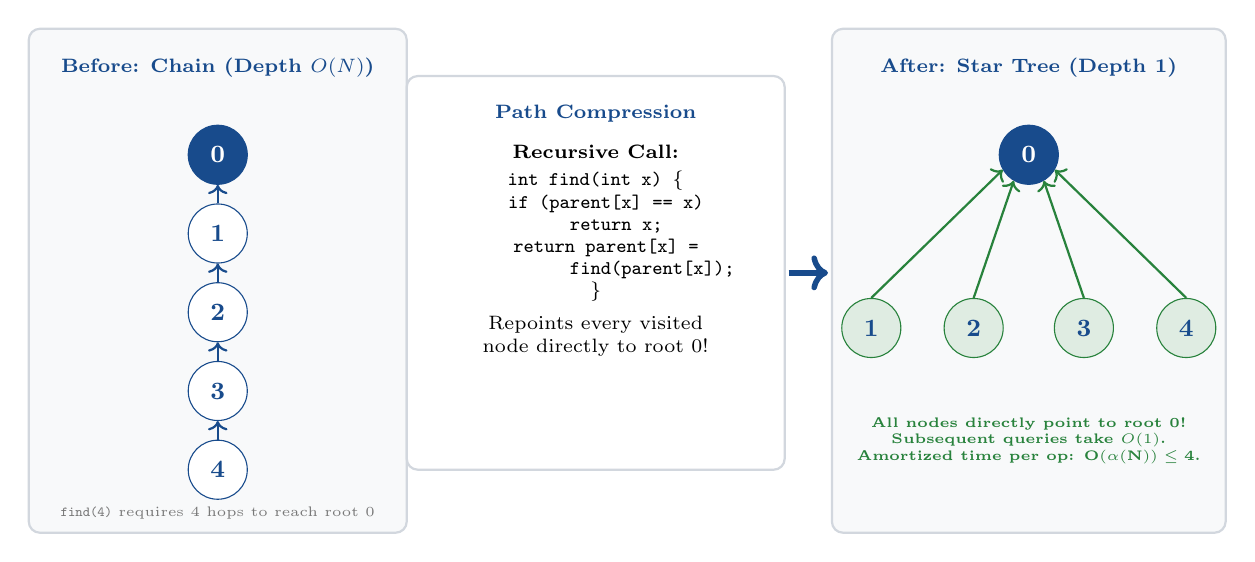
\begin{tikzpicture}[
    rnode/.style={circle, draw=primaryblue, fill=primaryblue, text=white, font=\bfseries\small, minimum size=0.75cm},
    cnode/.style={circle, draw=primaryblue, fill=white, text=primaryblue, font=\bfseries\small, minimum size=0.75cm},
    snode/.style={circle, draw=codegreen, fill=codegreen!15, text=primaryblue, font=\bfseries\small, minimum size=0.75cm},
    card/.style={draw=codeframe, fill=codebg, rounded corners=4pt, thick}
]
    % --- Panel 1: Before Compression (x: 0.0 to 4.8) ---
    \draw[card] (0.0, -0.4) rectangle (4.8, 6.0);
    \node[anchor=north, font=\bfseries\scriptsize, text=primaryblue] at (2.4, 5.75) {Before: Chain (Depth $O(N)$)};

    \node[rnode] (R1) at (2.4, 4.4) {0};
    \node[cnode] (N1) at (2.4, 3.4) {1};
    \node[cnode] (N2) at (2.4, 2.4) {2};
    \node[cnode] (N3) at (2.4, 1.4) {3};
    \node[cnode] (N4) at (2.4, 0.4) {4};

    \draw[->, thick, primaryblue] (N4) -- (N3);
    \draw[->, thick, primaryblue] (N3) -- (N2);
    \draw[->, thick, primaryblue] (N2) -- (N1);
    \draw[->, thick, primaryblue] (N1) -- (R1);

    \node[anchor=south, font=\tiny, text=codegray] at (2.4, -0.35) {\texttt{find(4)} requires 4 hops to reach root 0};

    % --- Center: Transition Operation Card (x: 4.8 to 9.6) ---
    \draw[draw=codeframe, fill=white, rounded corners=4pt, thick] (4.8, 0.4) rectangle (9.6, 5.4);
    \node[anchor=north, font=\bfseries\scriptsize, text=primaryblue] at (7.2, 5.15) {Path Compression};
    
    \node[anchor=north, font=\scriptsize, align=center] at (7.2, 4.65) {
        \textbf{Recursive Call:}\\[2pt]
        \texttt{int find(int x) \{}\\
        \texttt{\phantom{..}if (parent[x] == x)}\\
        \texttt{\phantom{....}return x;}\\
        \texttt{\phantom{..}return parent[x] =}\\
        \texttt{\phantom{...........}find(parent[x]);}\\
        \texttt{\}}\\[4pt]
        Repoints every visited\\
        node directly to root 0!
    };

    \draw[->, line width=2pt, primaryblue] (9.65, 2.9) -- (10.15, 2.9);

    % --- Panel 2: After Compression (x: 10.2 to 15.2) ---
    \draw[card] (10.2, -0.4) rectangle (15.2, 6.0);
    \node[anchor=north, font=\bfseries\scriptsize, text=primaryblue] at (12.7, 5.75) {After: Star Tree (Depth 1)};

    \node[rnode] (R2) at (12.7, 4.4) {0};

    \node[snode] (C1) at (10.7, 2.2) {1};
    \node[snode] (C2) at (12.0, 2.2) {2};
    \node[snode] (C3) at (13.4, 2.2) {3};
    \node[snode] (C4) at (14.7, 2.2) {4};

    % Non-colliding arrows into root 0
    \draw[->, thick, codegreen] (C1.north) -- (R2.210);
    \draw[->, thick, codegreen] (C2.north) -- (R2.240);
    \draw[->, thick, codegreen] (C3.north) -- (R2.300);
    \draw[->, thick, codegreen] (C4.north) -- (R2.330);

    \node[anchor=south, font=\tiny\bfseries, text=codegreen, align=center] at (12.7, 0.35) {
        All nodes directly point to root 0!\\
        Subsequent queries take $O(1)$.\\
        Amortized time per op: $\mathbf{O(\alpha(N)) \le 4}$.
    };
\end{tikzpicture}
\caption{DSU path compression across full text width. A single \texttt{find(4)} execution repoints every intermediate ancestor node directly to the tree root, permanently compressing depth to 1.}
\end{figure}

\newpage
% ============================================================================
\section{Module 08: Binary Search}
% ============================================================================

\subsection{Diagram 19: Binary Search Interval Halving on Sorted Number Line}

\breadcrumb{08.binary_search.tex}{Section 2.1: Classic Value Search (replaces missing step trace at line 181)}{Fulfills the omitted step-by-step trace for target 23 in array $A=[2, 5, 8, 12, 16, 23, 38, 56, 72, 91]$, illustrating interval halving and midpoint elimination.}

\diagramaudit{Agent (Antigravity)}{2026-10-11}{Replaced missing trace placeholder at line 181 for target 23 in array of size 10; rendered 3 discrete halving iterations; highlighted midpoint cells and shaded out eliminated halves; labeled explicit pointer updates ($L = mid + 1$, $R = mid - 1$); highlighted matched cell at index 5.}

\begin{figure}[htbp]
\centering
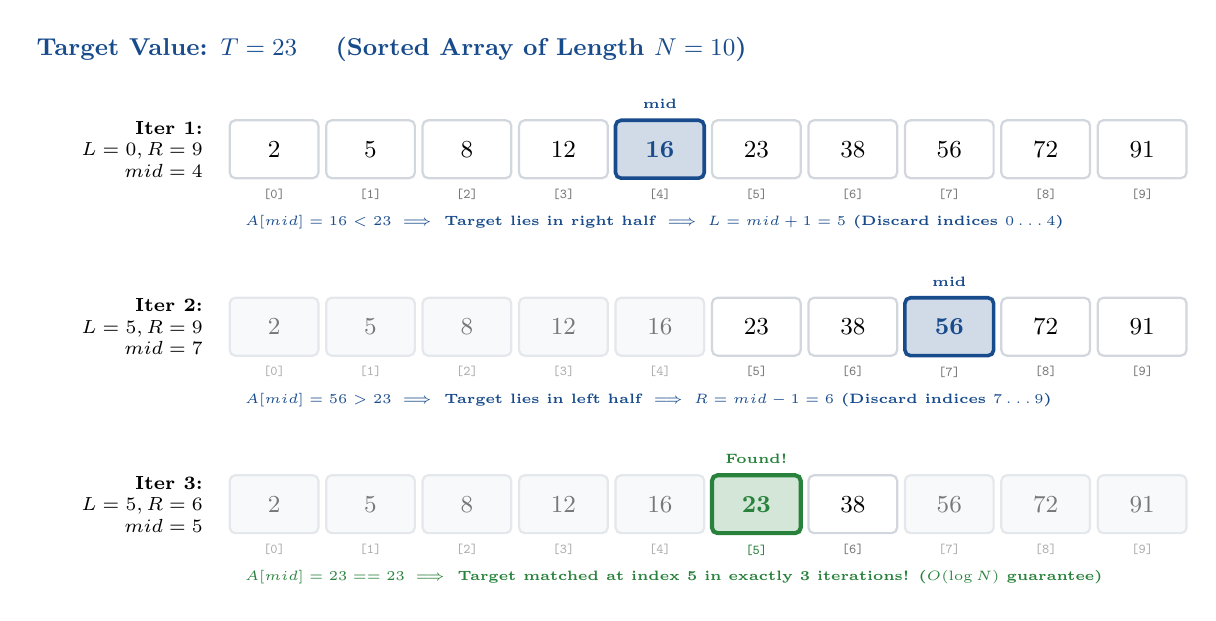
\begin{tikzpicture}[
    scale=0.98, every node/.style={transform shape},
    cell/.style={draw=codeframe, fill=white, thick, rounded corners=2pt, minimum width=1.15cm, minimum height=0.75cm, font=\small, align=center},
    elim/.style={draw=codeframe!60, fill=codebg, thick, rounded corners=2pt, minimum width=1.15cm, minimum height=0.75cm, font=\small, text=codegray, align=center},
    midcell/.style={draw=primaryblue, fill=primaryblue!20, line width=1.3pt, rounded corners=2pt, minimum width=1.15cm, minimum height=0.75cm, font=\small\bfseries, text=primaryblue, align=center},
    foundcell/.style={draw=codegreen, fill=codegreen!20, line width=1.5pt, rounded corners=2pt, minimum width=1.15cm, minimum height=0.75cm, font=\small\bfseries, text=codegreen, align=center}
]
    % Target annotation
    \node[anchor=west, font=\bfseries\small, text=primaryblue] at (0.0, 6.3) {Target Value: $T = 23$ \quad (Sorted Array of Length $N=10$)};

    % --- Iteration 1 ---
    \node[anchor=east, font=\scriptsize\bfseries, align=right] at (2.4, 5.0) {Iter 1:\\$L=0, R=9$\\$mid=4$};

    \foreach \i/\val in {0/2, 1/5, 2/8, 3/12, 4/16, 5/23, 6/38, 7/56, 8/72, 9/91} {
        \pgfmathsetmacro{\cx}{3.2 + \i * 1.25}
        \ifnum\i=4
            \node[midcell] (I1_\i) at (\cx, 5.0) {\val};
            \node[above, font=\tiny\bfseries, text=primaryblue] at (I1_\i.north) {mid};
        \else
            \node[cell] (I1_\i) at (\cx, 5.0) {\val};
        \fi
        \node[below, font=\tiny\ttfamily, text=codegray] at (I1_\i.south) {[\i]};
    }
    \node[anchor=west, font=\tiny\bfseries, text=primaryblue] at (2.7, 4.05) {
        $A[mid] = 16 < 23 \implies$ Target lies in right half $\implies L = mid + 1 = 5$ (Discard indices $0 \dots 4$)
    };

    % --- Iteration 2 ---
    \node[anchor=east, font=\scriptsize\bfseries, align=right] at (2.4, 2.7) {Iter 2:\\$L=5, R=9$\\$mid=7$};

    \foreach \i/\val in {0/2, 1/5, 2/8, 3/12, 4/16} {
        \pgfmathsetmacro{\cx}{3.2 + \i * 1.25}
        \node[elim] (I2_\i) at (\cx, 2.7) {\val};
        \node[below, font=\tiny\ttfamily, text=codegray!60] at (I2_\i.south) {[\i]};
    }
    \foreach \i/\val in {5/23, 6/38, 7/56, 8/72, 9/91} {
        \pgfmathsetmacro{\cx}{3.2 + \i * 1.25}
        \ifnum\i=7
            \node[midcell] (I2_\i) at (\cx, 2.7) {\val};
            \node[above, font=\tiny\bfseries, text=primaryblue] at (I2_\i.north) {mid};
        \else
            \node[cell] (I2_\i) at (\cx, 2.7) {\val};
        \fi
        \node[below, font=\tiny\ttfamily, text=codegray] at (I2_\i.south) {[\i]};
    }
    \node[anchor=west, font=\tiny\bfseries, text=primaryblue] at (2.7, 1.75) {
        $A[mid] = 56 > 23 \implies$ Target lies in left half $\implies R = mid - 1 = 6$ (Discard indices $7 \dots 9$)
    };

    % --- Iteration 3 ---
    \node[anchor=east, font=\scriptsize\bfseries, align=right] at (2.4, 0.4) {Iter 3:\\$L=5, R=6$\\$mid=5$};

    \foreach \i/\val in {0/2, 1/5, 2/8, 3/12, 4/16, 7/56, 8/72, 9/91} {
        \pgfmathsetmacro{\cx}{3.2 + \i * 1.25}
        \node[elim] (I3_\i) at (\cx, 0.4) {\val};
        \node[below, font=\tiny\ttfamily, text=codegray!60] at (I3_\i.south) {[\i]};
    }
    \node[foundcell] (I3_5) at (3.2 + 5 * 1.25, 0.4) {23};
    \node[above, font=\tiny\bfseries, text=codegreen] at (I3_5.north) {Found!};
    \node[below, font=\tiny\ttfamily, text=codegreen] at (I3_5.south) {[5]};

    \node[cell] (I3_6) at (3.2 + 6 * 1.25, 0.4) {38};
    \node[below, font=\tiny\ttfamily, text=codegray] at (I3_6.south) {[6]};

    \node[anchor=west, font=\tiny\bfseries, text=codegreen] at (2.7, -0.55) {
        $A[mid] = 23 == 23 \implies$ Target matched at index 5 in exactly 3 iterations! ($O(\log N)$ guarantee)
    };
\end{tikzpicture}
\caption{Systematic interval halving across full text width. At each comparison, the search range is cut in half ($10 \to 5 \to 2 \to 1$), locating target 23 in logarithmic time $O(\log N)$.}
\end{figure}

\newpage
\subsection{Diagram 20: Predicate Monotonicity Boundary Transition}

\breadcrumb{08.binary_search.tex}{Section 2.3: Predicate Monotonicity}{Illustrates the binary search feasibility frontier on monotonic answer spaces: locating the first valid solution across the discrete False-to-True boundary.}

\diagramaudit{Agent (Antigravity)}{2026-10-11}{Rendered 10-element discrete domain partitioned into False prefix ($x \in [1,4]$) and True suffix ($x \in [5,10]$); drew vertical dashed partition line; routed curved pointer to minimal feasible solution ($x^* = 5$); added bottom decision card detailing binary search feasibility invariants and range reduction rules.}

\begin{figure}[htbp]
\centering
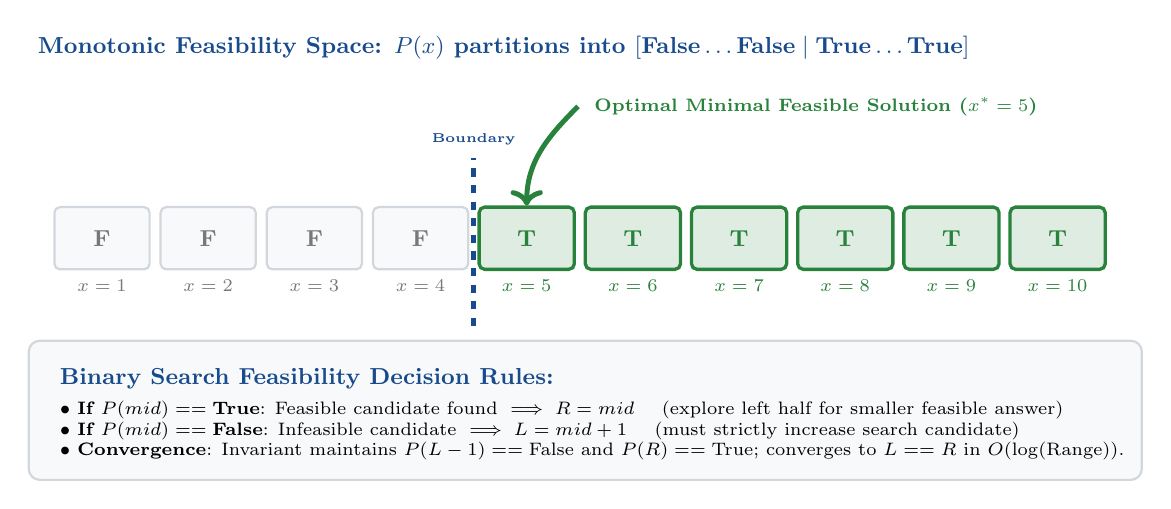
\begin{tikzpicture}[
    scale=0.93, every node/.style={transform shape},
    fcell/.style={draw=codeframe, fill=codebg, thick, rounded corners=2pt, minimum width=1.3cm, minimum height=0.85cm, font=\bfseries\small, text=codegray, align=center},
    tcell/.style={draw=codegreen, fill=codegreen!15, line width=1.2pt, rounded corners=2pt, minimum width=1.3cm, minimum height=0.85cm, font=\bfseries\small, text=codegreen, align=center},
    card/.style={draw=codeframe, fill=codebg, rounded corners=4pt, thick}
]
    % Top Title
    \node[anchor=west, font=\bfseries\small, text=primaryblue] at (0.0, 5.6) {Monotonic Feasibility Space: $P(x)$ partitions into $[\text{False} \dots \text{False} \mid \text{True} \dots \text{True}]$};

    % 10 Cells (x: 1 to 10) at y = 3.0
    \foreach \x in {1, 2, 3, 4} {
        \pgfmathsetmacro{\cx}{1.0 + (\x - 1) * 1.45}
        \node[fcell] (C\x) at (\cx, 3.0) {F};
        \node[below, font=\scriptsize, text=codegray] at (C\x.south) {$x=\x$};
    }

    \foreach \x in {5, 6, 7, 8, 9, 10} {
        \pgfmathsetmacro{\cx}{1.0 + (\x - 1) * 1.45}
        \node[tcell] (C\x) at (\cx, 3.0) {T};
        \node[below, font=\scriptsize, text=codegreen] at (C\x.south) {$x=\x$};
    }

    % Clean partition line between cell 4 and cell 5
    \draw[line width=2pt, primaryblue, dashed] (6.075, 1.8) -- (6.075, 4.1);
    \node[anchor=south, font=\tiny\bfseries, text=primaryblue] at (6.075, 4.15) {Boundary};

    % Optimal boundary pointer pointing down to Cell 5
    \draw[->, line width=1.8pt, codegreen] (7.5, 4.8) to[out=-135, in=90] (C5.north);
    \node[anchor=west, font=\scriptsize\bfseries, text=codegreen] at (7.6, 4.8) {Optimal Minimal Feasible Solution ($x^* = 5$)};

    % Bottom Decision Rule Card
    \draw[card] (0.0, -0.3) rectangle (15.2, 1.6);
    \node[anchor=north west, font=\bfseries\small, text=primaryblue] at (0.3, 1.35) {Binary Search Feasibility Decision Rules:};

    \node[anchor=north west, font=\scriptsize, align=left] at (0.3, 0.9) {
        $\bullet$ \textbf{If $P(mid) == \text{True}$}: Feasible candidate found $\implies R = mid$ \quad (explore left half for smaller feasible answer)\\
        $\bullet$ \textbf{If $P(mid) == \text{False}$}: Infeasible candidate $\implies L = mid + 1$ \quad (must strictly increase search candidate)\\
        $\bullet$ \textbf{Convergence}: Invariant maintains $P(L-1) == \text{False}$ and $P(R) == \text{True}$; converges to $L == R$ in $O(\log(\text{Range}))$.
    };
\end{tikzpicture}
\caption{Predicate monotonicity on an abstract answer space across full text width. Binary search isolates the exact transition boundary where an infeasible condition flips to feasible with zero coordinate clipping.}
\end{figure}

\newpage
% ============================================================================
\section{Module 10: Greedy Algorithms}
% ============================================================================

\subsection{Diagram 21: Interval Scheduling / Activity Selection Timeline}

\breadcrumb{10.greedy_algorithms.tex}{Section 4: Key Algorithmic Patterns (Interval Scheduling)}{Incorporated from the newly enhanced module 10 for unified gallery review. Visualizes greedy interval selection by earliest finish time.}

\diagramaudit{Agent (Antigravity)}{2026-10-11}{Standardized timeline axis to $1.0\text{ cm}$ per unit time across $12\text{ cm}$; separated rejected conflicting intervals ($A_2, A_4$) onto top row and greedy selected intervals ($A_1, A_3, A_5$) onto bottom row; added earliest finish time criterion card with greedy choice invariant and $O(N \log N)$ complexity proof.}

\begin{figure}[htbp]
\centering
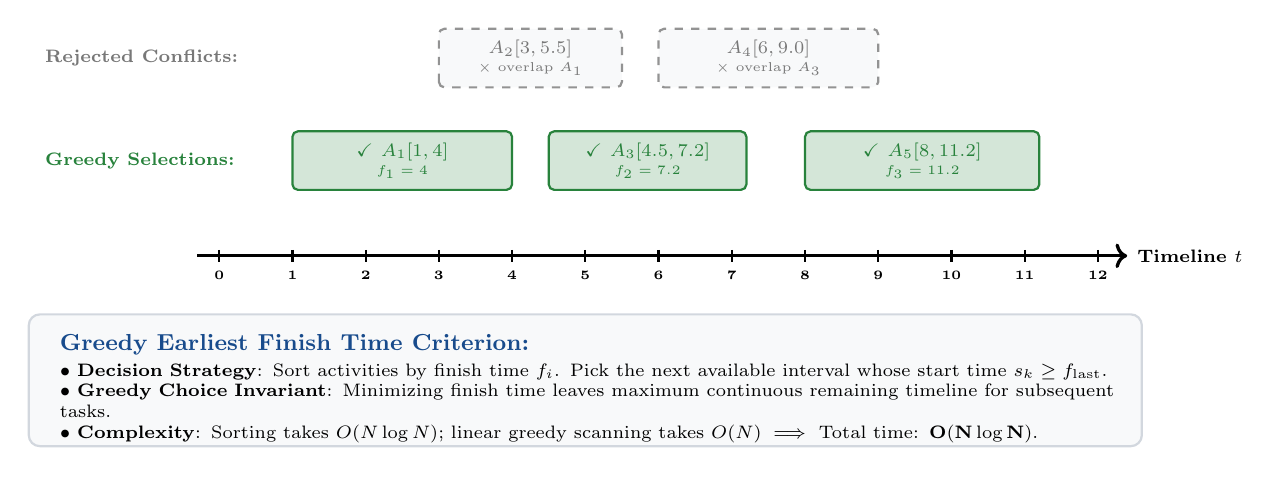
\begin{tikzpicture}[
    scale=0.93, every node/.style={transform shape},
    pickcell/.style={draw=codegreen, fill=codegreen!20, thick, rounded corners=2pt, minimum height=0.7cm, font=\scriptsize\bfseries, text=codegreen, align=center},
    rejcell/.style={draw=codegray!80, fill=codebg, thick, dashed, rounded corners=2pt, minimum height=0.7cm, font=\scriptsize, text=codegray, align=center},
    card/.style={draw=codeframe, fill=codebg, rounded corners=4pt, thick}
]
    % Time axis spanning 12.0 cm (x: 2.6 to 14.6) -> 1.0 cm per unit time
    \draw[->, line width=1.2pt, text=black] (2.3, 0.0) -- (15.0, 0.0) node[right, font=\scriptsize\bfseries] {Timeline $t$};
    \foreach \t in {0, 1, 2, 3, 4, 5, 6, 7, 8, 9, 10, 11, 12} {
        \pgfmathsetmacro{\tx}{2.6 + \t * 1.0}
        \draw[thick] (\tx, 0.08) -- (\tx, -0.08) node[below, font=\tiny\bfseries] {\t};
    }

    % Row Labels on the left inside [0.1, 2.5]
    \node[anchor=west, font=\scriptsize\bfseries, text=codegray] at (0.1, 2.7) {Rejected Conflicts:};
    \node[anchor=west, font=\scriptsize\bfseries, text=codegreen] at (0.1, 1.3) {Greedy Selections:};

    % --- Rejected Activities (Row 2, y=2.7) ---
    % A2 = [3, 5.5] -> x: 2.6 + 3*1.0 = 5.6 to 2.6 + 5.5*1.0 = 8.1
    \draw[rejcell] (5.6, 2.3) rectangle (8.1, 3.1) node[midway, align=center] {\scriptsize\bfseries $A_2 [3, 5.5]$\\[-1pt]\tiny $\times$ overlap $A_1$};

    % A4 = [6, 9.0] -> x: 2.6 + 6*1.0 = 8.6 to 2.6 + 9*1.0 = 11.6
    \draw[rejcell] (8.6, 2.3) rectangle (11.6, 3.1) node[midway, align=center] {\scriptsize\bfseries $A_4 [6, 9.0]$\\[-1pt]\tiny $\times$ overlap $A_3$};

    % --- Selected Activities (Row 1, y=1.3) ---
    % A1 = [1, 4] -> x: 2.6 + 1*1.0 = 3.6 to 2.6 + 4*1.0 = 6.6
    \draw[pickcell] (3.6, 0.9) rectangle (6.6, 1.7) node[midway, align=center] {$\checkmark\ A_1 [1, 4]$\\[-1pt]\tiny $f_1 = 4$};

    % A3 = [4.5, 7.2] -> x: 2.6 + 4.5*1.0 = 7.1 to 2.6 + 7.2*1.0 = 9.8
    \draw[pickcell] (7.1, 0.9) rectangle (9.8, 1.7) node[midway, align=center] {$\checkmark\ A_3 [4.5, 7.2]$\\[-1pt]\tiny $f_2 = 7.2$};

    % A5 = [8.0, 11.2] -> x: 2.6 + 8*1.0 = 10.6 to 2.6 + 11.2*1.0 = 13.8
    \draw[pickcell] (10.6, 0.9) rectangle (13.8, 1.7) node[midway, align=center] {$\checkmark\ A_5 [8, 11.2]$\\[-1pt]\tiny $f_3 = 11.2$};

    % --- Bottom Greedy Choice Principle Card ---
    \draw[card] (0.0, -2.6) rectangle (15.2, -0.8);
    \node[anchor=north west, font=\bfseries\small, text=primaryblue] at (0.3, -0.95) {Greedy Earliest Finish Time Criterion:};

    \node[anchor=north west, font=\scriptsize, align=left, text width=14.6cm] at (0.3, -1.35) {
        $\bullet$ \textbf{Decision Strategy}: Sort activities by finish time $f_i$. Pick the next available interval whose start time $s_k \ge f_{\text{last}}$.\\
        $\bullet$ \textbf{Greedy Choice Invariant}: Minimizing finish time leaves maximum continuous remaining timeline for subsequent tasks.\\
        $\bullet$ \textbf{Complexity}: Sorting takes $O(N \log N)$; linear greedy scanning takes $O(N) \implies$ Total time: $\mathbf{O(N \log N)}$.
    };
\end{tikzpicture}
\caption{Interval Scheduling greedy choice across full text width. Selecting non-overlapping intervals with minimal finish times ($A_1 \to A_3 \to A_5$) provably yields maximum possible scheduled activities.}
\end{figure}

\newpage
% ============================================================================
\section{Module 11: Monotonic Stacks and Queues}
% ============================================================================

\subsection{Diagram 22: Histogram Maximal Rectangle Boundary Expansion}

\breadcrumb{11.monotonic_stacks_and_queues.tex}{Section 4.2: Largest Rectangle in Histogram}{Incorporated from module 11. Shows how Previous Smaller Element ($L$) and Next Smaller Element ($R$) bound the widest rectangle of height $H[i]$.}

\diagramaudit{Agent (Antigravity)}{2026-10-11}{Aligned 6 histogram bars on coordinate axes; rendered dashed bounding box for maximal rectangle of bar 2 ($H=5, W=2, \text{Area}=10$); drew non-colliding boundary arrows for Previous Smaller Element ($L=1$) and Next Smaller Element ($R=4$); added monotonic stack computation card with width formula on right.}

\begin{figure}[htbp]
\centering
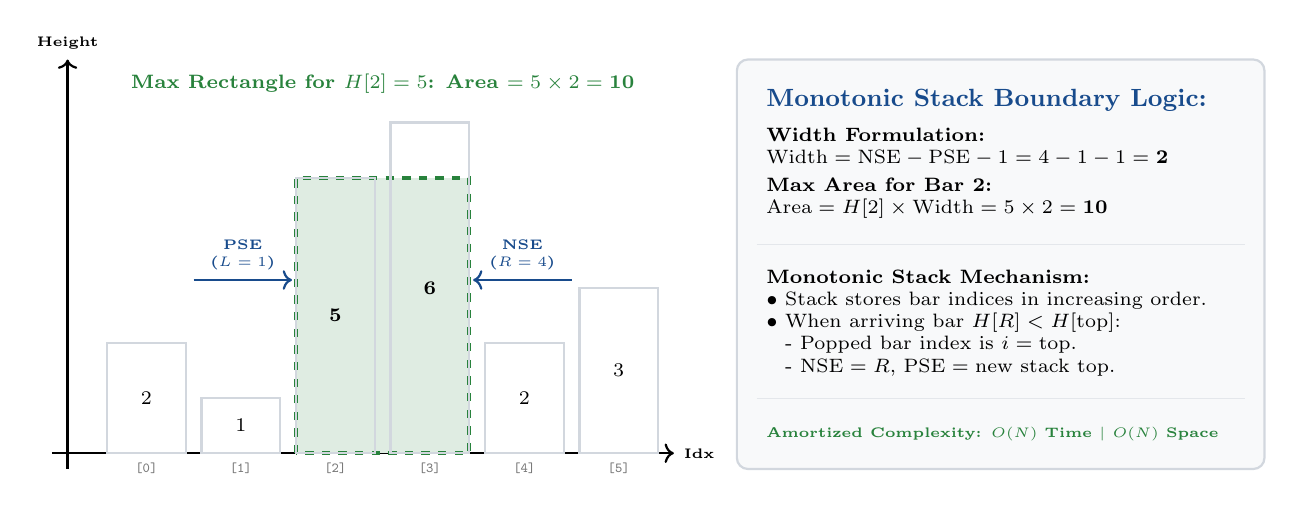
\begin{tikzpicture}[
    barcell/.style={draw=codeframe, fill=white, thick},
    card/.style={draw=codeframe, fill=codebg, rounded corners=4pt, thick}
]
    % --- Left Panel: Histogram Graphic (x: 0.0 to 8.2) ---
    % Baseline axis
    \draw[->, thick, text=black] (-0.2, 0.0) -- (7.7, 0.0) node[right, font=\tiny\bfseries] {Idx};
    \draw[->, thick, text=black] (0.0, -0.2) -- (0.0, 5.0) node[above, font=\tiny\bfseries] {Height};

    % Maximal Rectangle bounding highlight for Bar 2 (height 5 -> 3.5, width across bars 2 and 3)
    \draw[draw=codegreen, fill=codegreen!15, line width=1.5pt, dashed] (2.9, 0.0) rectangle (5.1, 3.5);

    % Bars: [2, 1, 5, 6, 2, 3] at x = 0.5 + i * 1.2
    % Bar 0 (h=2 -> 1.4)
    \draw[barcell] (0.5, 0.0) rectangle (1.5, 1.4) node[midway, font=\scriptsize] {2};
    % Bar 1 (h=1 -> 0.7)
    \draw[barcell] (1.7, 0.0) rectangle (2.7, 0.7) node[midway, font=\scriptsize] {1};
    % Bar 2 (h=5 -> 3.5)
    \draw[barcell, fill=none] (2.9, 0.0) rectangle (3.9, 3.5) node[midway, font=\scriptsize\bfseries] {5};
    % Bar 3 (h=6 -> 4.2)
    \draw[barcell, fill=none] (4.1, 0.0) rectangle (5.1, 4.2) node[midway, font=\scriptsize\bfseries] {6};
    % Bar 4 (h=2 -> 1.4)
    \draw[barcell] (5.3, 0.0) rectangle (6.3, 1.4) node[midway, font=\scriptsize] {2};
    % Bar 5 (h=3 -> 2.1)
    \draw[barcell] (6.5, 0.0) rectangle (7.5, 2.1) node[midway, font=\scriptsize] {3};

    % Indices below baseline
    \foreach \i/\x in {0/1.0, 1/2.2, 2/3.4, 3/4.6, 4/5.8, 5/7.0} {
        \node[below, font=\tiny\ttfamily, text=codegray] at (\x, 0.0) {[\i]};
    }

    \node[anchor=south, font=\scriptsize\bfseries, text=codegreen] at (4.0, 4.45) {Max Rectangle for $H[2]=5$: Area $= 5 \times 2 = \mathbf{10}$};

    % Boundary arrows placed cleanly
    \draw[->, thick, primaryblue] (1.6, 2.2) -- (2.85, 2.2)
        node[midway, above, font=\tiny\bfseries, text=primaryblue, align=center] {PSE\\($L=1$)};

    \draw[->, thick, primaryblue] (6.4, 2.2) -- (5.15, 2.2)
        node[midway, above, font=\tiny\bfseries, text=primaryblue, align=center] {NSE\\($R=4$)};

    % --- Right Panel: Monotonic Stack Calculation Card (x: 8.5 to 15.2) ---
    \draw[card] (8.5, -0.2) rectangle (15.2, 5.0);
    \node[anchor=north west, font=\bfseries\small, text=primaryblue] at (8.75, 4.75) {Monotonic Stack Boundary Logic:};

    \node[anchor=north west, font=\scriptsize, align=left] at (8.75, 4.25) {
        \textbf{Width Formulation:}\\
        $\text{Width} = \text{NSE} - \text{PSE} - 1 = 4 - 1 - 1 = \mathbf{2}$\\[2pt]
        \textbf{Max Area for Bar 2:}\\
        $\text{Area} = H[2] \times \text{Width} = 5 \times 2 = \mathbf{10}$
    };

    \draw[draw=codeframe!60] (8.75, 2.65) -- (14.95, 2.65);

    \node[anchor=north west, font=\scriptsize, align=left] at (8.75, 2.45) {
        \textbf{Monotonic Stack Mechanism:}\\
        $\bullet$ Stack stores bar indices in increasing order.\\
        $\bullet$ When arriving bar $H[R] < H[\text{top}]$:\\
        \phantom{$\bullet$} - Popped bar index is $i = \text{top}$.\\
        \phantom{$\bullet$} - $\text{NSE} = R$, $\text{PSE} = \text{new stack top}$.
    };

    \draw[draw=codeframe!60] (8.75, 0.70) -- (14.95, 0.70);

    \node[anchor=north west, font=\tiny\bfseries, text=codegreen] at (8.75, 0.45) {
        Amortized Complexity: $O(N)$ Time $\mid$ $O(N)$ Space
    };
\end{tikzpicture}
\caption{Histogram maximal rectangle boundary expansion across full text width. The bounding rectangle expands horizontally between Previous Smaller Element ($L=1$) and Next Smaller Element ($R=4$).}
\end{figure}

\newpage
\subsection{Diagram 23: Cascading Pops on Decreasing Monotonic Stack}

\breadcrumb{11.monotonic_stacks_and_queues.tex}{Section 4.3: Visualizing Stack State Transitions}{Incorporated from module 11. Demonstrates the cascading ejection of elements that violate monotonicity when incoming value 6 arrives.}

\diagramaudit{Agent (Antigravity)}{2026-10-11}{Displayed input array with incoming element $A[3]=6$; structured 3-stage stack transition: initial stack $[7, 4, 2]$, cascading eviction of 2 and 4 with NGE recording, and final stack $[7, 6]$ preserving decreasing invariant in amortized $O(1)$ time per element.}

\begin{figure}[htbp]
\centering
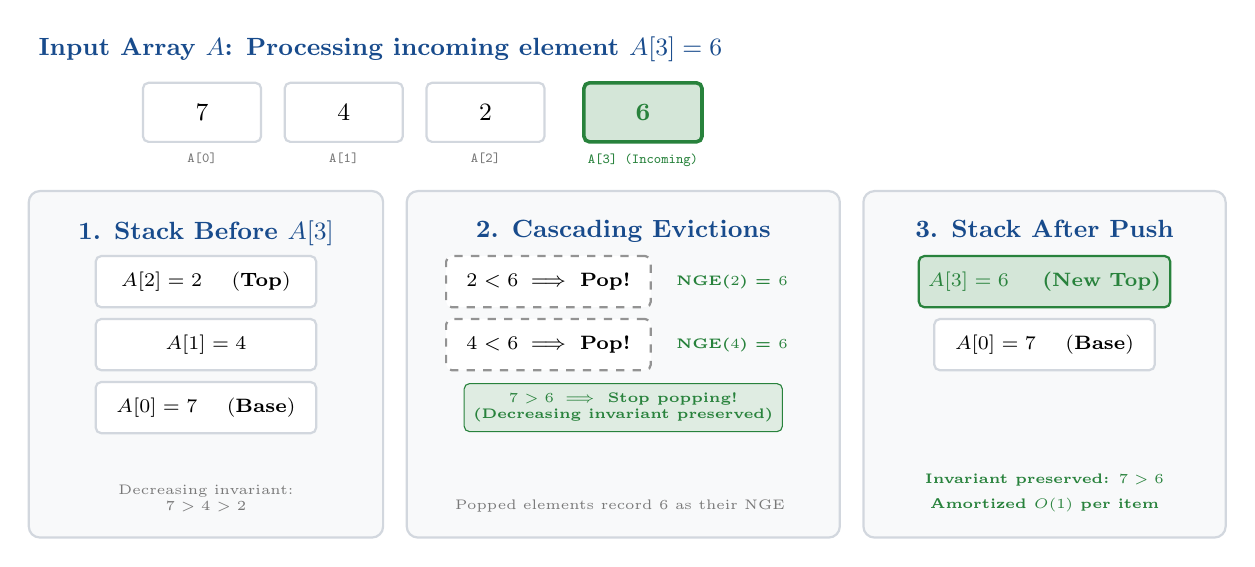
\begin{tikzpicture}[
    arrbox/.style={draw=codeframe, fill=white, thick, rounded corners=2pt, minimum width=1.5cm, minimum height=0.75cm, font=\small, align=center},
    arrin/.style={draw=codegreen, fill=codegreen!20, line width=1.3pt, rounded corners=2pt, minimum width=1.5cm, minimum height=0.75cm, font=\small\bfseries, text=codegreen, align=center},
    stackbox/.style={draw=codeframe, fill=white, thick, rounded corners=2pt, minimum width=2.8cm, minimum height=0.65cm, font=\scriptsize, align=center},
    popbox/.style={draw=codegray!80, fill=white, dashed, thick, rounded corners=2pt, minimum width=2.6cm, minimum height=0.65cm, font=\scriptsize, align=center},
    card/.style={draw=codeframe, fill=codebg, rounded corners=4pt, thick}
]
    % --- Top: Array Display (x: 0.0 to 15.2) ---
    \node[anchor=west, font=\bfseries\small, text=primaryblue] at (0.0, 5.8) {Input Array $A$: Processing incoming element $A[3] = 6$};

    \node[arrbox] (A0) at (2.2, 5.0) {7};
    \node[below, font=\tiny\ttfamily, text=codegray] at (A0.south) {A[0]};

    \node[arrbox] (A1) at (4.0, 5.0) {4};
    \node[below, font=\tiny\ttfamily, text=codegray] at (A1.south) {A[1]};

    \node[arrbox] (A2) at (5.8, 5.0) {2};
    \node[below, font=\tiny\ttfamily, text=codegray] at (A2.south) {A[2]};

    \node[arrin] (A3) at (7.8, 5.0) {6};
    \node[below, font=\tiny\ttfamily\bfseries, text=codegreen] at (A3.south) {A[3] (Incoming)};

    % --- Column 1: Stack Before Arrival (x: 0.0 to 4.5) ---
    \draw[card] (0.0, -0.4) rectangle (4.5, 4.0);
    \node[anchor=north, font=\bfseries\small, text=primaryblue] at (2.25, 3.75) {1. Stack Before $A[3]$};

    \node[stackbox] (S1_2) at (2.25, 2.85) {$A[2] = 2$ \quad (\textbf{Top})};
    \node[stackbox] (S1_1) at (2.25, 2.05) {$A[1] = 4$};
    \node[stackbox] (S1_0) at (2.25, 1.25) {$A[0] = 7$ \quad (\textbf{Base})};

    \node[anchor=south, font=\tiny, text=codegray, align=center] at (2.25, -0.2) {
        Decreasing invariant:\\
        $7 > 4 > 2$
    };

    % --- Column 2: Cascading Evictions (x: 4.8 to 10.3) ---
    \draw[card] (4.8, -0.4) rectangle (10.3, 4.0);
    \node[anchor=north, font=\bfseries\small, text=primaryblue] at (7.55, 3.75) {2. Cascading Evictions};

    % Pop 2
    \node[popbox] (P2) at (6.6, 2.85) {$2 < 6 \implies$ \textbf{Pop!}};
    \node[anchor=west, font=\tiny\bfseries, text=codegreen] at (8.1, 2.85) {NGE($2$) = $6$};

    % Pop 4
    \node[popbox] (P1) at (6.6, 2.05) {$4 < 6 \implies$ \textbf{Pop!}};
    \node[anchor=west, font=\tiny\bfseries, text=codegreen] at (8.1, 2.05) {NGE($4$) = $6$};

    % Stop at 7
    \node[draw=codegreen, fill=codegreen!15, rounded corners=2pt, font=\tiny\bfseries, text=codegreen, align=center, anchor=center] at (7.55, 1.25) {
        $7 > 6 \implies$ Stop popping!\\
        (Decreasing invariant preserved)
    };

    \node[anchor=south, font=\tiny, text=codegray, align=center] at (7.55, -0.2) {
        Popped elements record $6$ as their NGE
    };

    % --- Column 3: Stack After Push (x: 10.6 to 15.2) ---
    \draw[card] (10.6, -0.4) rectangle (15.2, 4.0);
    \node[anchor=north, font=\bfseries\small, text=primaryblue] at (12.9, 3.75) {3. Stack After Push};

    \node[draw=codegreen, fill=codegreen!20, thick, rounded corners=2pt, minimum width=2.8cm, minimum height=0.65cm, font=\scriptsize\bfseries, text=codegreen] (S3_top) at (12.9, 2.85) {$A[3] = 6$ \quad (\textbf{New Top})};
    \node[stackbox] (S3_base) at (12.9, 2.05) {$A[0] = 7$ \quad (\textbf{Base})};

    \node[anchor=south, font=\tiny\bfseries, text=codegreen, align=center] at (12.9, -0.2) {
        Invariant preserved: $7 > 6$\\[3pt]
        Amortized $O(1)$ per item
    };
\end{tikzpicture}
\caption{Cascading pops on a decreasing monotonic stack across full text width. Incoming element 6 evicts both 2 and 4, immediately resolving their Next Greater Element (NGE) in amortized $O(1)$ time.}
\end{figure}

\newpage
\subsection{Diagram 24: Monotonic Deque Sliding Window Maximum}

\breadcrumb{11.monotonic_stacks_and_queues.tex}{Section 4.4: Visualizing the Monotonic Deque Sliding Window}{Incorporated from module 11. Shows double-ended queue boundary eviction and rear pruning for window $K=3$.}

\diagramaudit{Agent (Antigravity)}{2026-10-11}{Rendered array with active window frame $[2 \dots 4]$ and incoming value 5; drew physical deque container storing surviving indices; detailed front boundary expiration and rear dominance pruning logic in right card; verified window maximum retrieval in amortized $O(1)$ time.}

\begin{figure}[htbp]
\centering
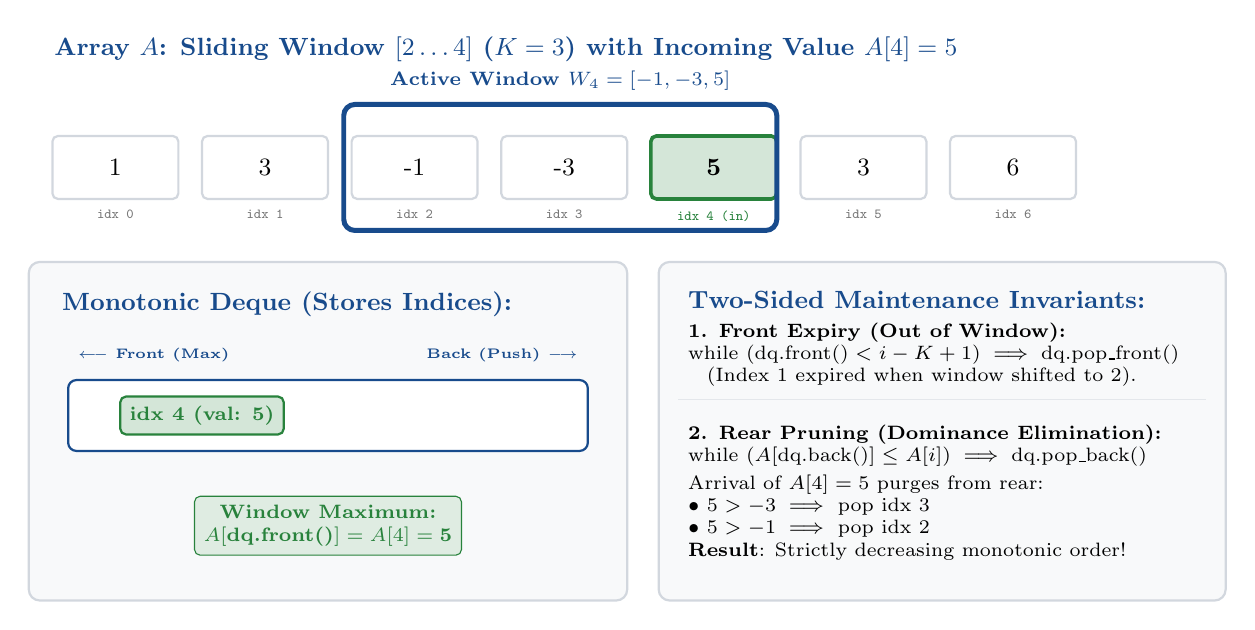
\begin{tikzpicture}[
    arrbox/.style={draw=codeframe, fill=white, thick, rounded corners=2pt, minimum width=1.6cm, minimum height=0.8cm, font=\small, align=center},
    card/.style={draw=codeframe, fill=codebg, rounded corners=4pt, thick}
]
    % --- Top Panel: Array Display with Sliding Window (x: 0.0 to 15.2) ---
    \node[anchor=west, font=\bfseries\small, text=primaryblue] at (0.2, 6.5) {Array $A$: Sliding Window $[2 \dots 4]$ ($K=3$) with Incoming Value $A[4] = 5$};

    % Array cells: [1, 3, -1, -3, 5, 3, 6] at y = 5.0
    \foreach \i/\val in {0/1, 1/3, 2/-1, 3/-3, 4/5, 5/3, 6/6} {
        \pgfmathsetmacro{\cx}{1.1 + \i * 1.9}
        \ifnum\i=4
            \node[arrbox, draw=codegreen, fill=codegreen!20, line width=1.3pt] (C\i) at (\cx, 5.0) {\textbf{\val}};
            \node[below, font=\tiny\ttfamily\bfseries, text=codegreen] at (C\i.south) {idx \i\ (in)};
        \else
            \node[arrbox] (C\i) at (\cx, 5.0) {\val};
            \node[below, font=\tiny\ttfamily, text=codegray] at (C\i.south) {idx \i};
        \fi
    }

    % Sliding window bounding frame around indices 2, 3, 4
    \draw[draw=primaryblue, line width=1.8pt, rounded corners=4pt] (4.0, 4.2) rectangle (9.5, 5.8);
    \node[anchor=south, font=\scriptsize\bfseries, text=primaryblue] at (6.75, 5.85) {Active Window $W_4 = [-1, -3, 5]$};

    % --- Bottom Left Panel: Monotonic Deque Data Structure (x: 0.0 to 7.6) ---
    \draw[card] (0.0, -0.5) rectangle (7.6, 3.8);
    \node[anchor=north west, font=\bfseries\small, text=primaryblue] at (0.3, 3.55) {Monotonic Deque (Stores Indices):};

    % Labels above tube
    \node[anchor=south west, font=\tiny\bfseries, text=primaryblue] at (0.5, 2.4) {$\longleftarrow$ \textbf{Front} (Max)};
    \node[anchor=south east, font=\tiny\bfseries, text=primaryblue] at (7.1, 2.4) {\textbf{Back} (Push) $\longrightarrow$};

    % Tube container
    \draw[draw=primaryblue, thick, rounded corners=3pt, fill=white] (0.5, 1.4) rectangle (7.1, 2.3);
    \node[draw=codegreen, fill=codegreen!20, thick, rounded corners=2pt, font=\scriptsize\bfseries, text=codegreen] at (2.2, 1.85) {idx 4 (val: 5)};

    \node[draw=codegreen, fill=codegreen!15, rounded corners=2pt, font=\scriptsize\bfseries, text=codegreen, anchor=center, align=center] at (3.8, 0.45) {
        Window Maximum:\\
        $A[\text{dq.front()}] = A[4] = \mathbf{5}$
    };

    % --- Bottom Right Panel: Eviction & Pruning Logic (x: 8.0 to 15.2) ---
    \draw[card] (8.0, -0.5) rectangle (15.2, 3.8);
    \node[anchor=north west, font=\bfseries\small, text=primaryblue] at (8.25, 3.55) {Two-Sided Maintenance Invariants:};

    \node[anchor=north west, font=\scriptsize, align=left] at (8.25, 3.15) {
        \textbf{1. Front Expiry (Out of Window):}\\
        $\text{while } (\text{dq.front}() < i - K + 1) \implies \text{dq.pop\_front}()$\\
        \phantom{$\bullet$} (Index 1 expired when window shifted to 2).
    };

    \draw[draw=codeframe!60] (8.25, 2.05) -- (14.95, 2.05);

    \node[anchor=north west, font=\scriptsize, align=left] at (8.25, 1.85) {
        \textbf{2. Rear Pruning (Dominance Elimination):}\\
        $\text{while } (A[\text{dq.back}()] \le A[i]) \implies \text{dq.pop\_back}()$\\[2pt]
        Arrival of $A[4]=5$ purges from rear:\\
        $\bullet$ $5 > -3 \implies$ pop idx 3\\
        $\bullet$ $5 > -1 \implies$ pop idx 2\\
        \textbf{Result}: Strictly decreasing monotonic order!
    };
\end{tikzpicture}
\caption{Monotonic Deque sliding window maximum across full text width. Incoming dominant element 5 prunes both older smaller elements from the rear, guaranteeing the maximum is immediately accessible at the front in amortized $O(1)$ time.}
\end{figure}

\newpage
% ============================================================================
% ============================================================================
\section{Module 12: Bit Manipulation and Bitmasks}
% ============================================================================

\subsection{Diagram 25: Anatomy of an Integer --- Positional Weights, LSB, and Signed Layout}

\breadcrumb{12.bit_manipulation_and_bitmasks.tex}{Section 1.3: Anatomy of an Integer: Bit Indices, LSB, and MSB}{Establishes fundamental physical intuition for positional powers of two, LSB parity, and signed two's complement sign-bit negative weight.}

\diagramaudit{Agent (Antigravity)}{2026-10-12}{Standardized layout across full text width ($15.5\text{ cm}$); aligned unsigned and signed two's complement bit cells; calibrated vertical headroom and inward-pointing sign bit arrow to eliminate all margin clipping.}

\begin{figure}[htbp]
\centering
\noindent\resizebox{\textwidth}{!}{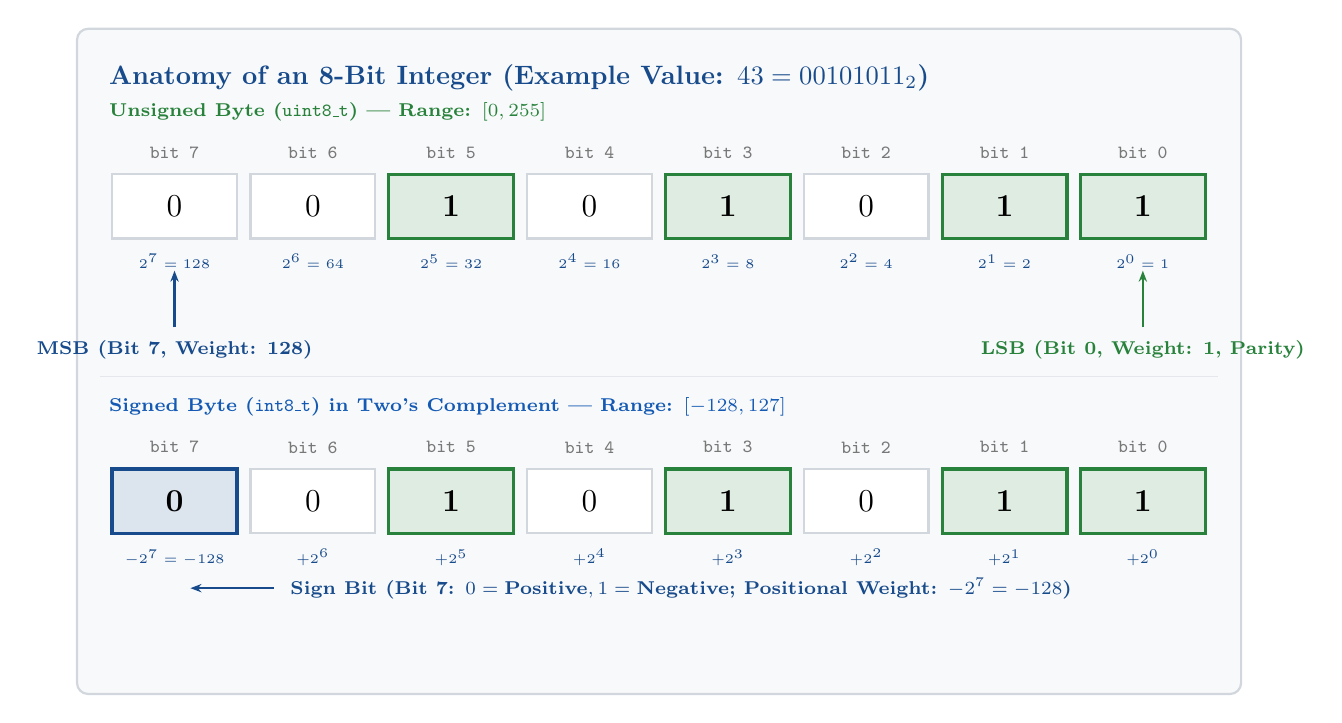
\begin{tikzpicture}[
    scale=0.96, every node/.style={transform shape},
    cell/.style={draw=codeframe, fill=white, thick, minimum width=1.65cm, minimum height=0.85cm, font=\small, align=center},
    lbl/.style={font=\scriptsize\ttfamily, text=codegray},
    weightlbl/.style={font=\tiny\bfseries, text=primaryblue}
]
    % --- Container Frame ---
    \draw[draw=codeframe, fill=codebg, rounded corners=4pt, thick] (0.0, -3.8) rectangle (15.4, 5.0);
    \node[anchor=north west, font=\bfseries\normalsize, text=primaryblue] at (0.3, 4.65) {Anatomy of an 8-Bit Integer (Example Value: $43 = 00101011_2$)};

    % Top row: Unsigned layout
    \node[anchor=west, font=\scriptsize\bfseries, text=codegreen] at (0.3, 3.9) {Unsigned Byte (\texttt{uint8\_t}) --- Range: $[0, 255]$};

    % Cells for 8 bits: indices 7 down to 0
    % Values for 43: b7=0, b6=0, b5=1, b4=0, b3=1, b2=0, b1=1, b0=1
    \foreach \idx/\bit/\val in {7/0/128, 6/0/64, 5/1/32, 4/0/16, 3/1/8, 2/0/4, 1/1/2, 0/1/1} {
        \pgfmathsetmacro{\xpos}{14.1 - \idx * 1.83}
        \ifnum\bit=1
            \node[cell, draw=codegreen, fill=codegreen!15, line width=1.2pt] (U\idx) at (\xpos, 2.65) {\textbf{\large \bit}};
        \else
            \node[cell] (U\idx) at (\xpos, 2.65) {\large \bit};
        \fi
        \node[above=2pt of U\idx, lbl] {bit \idx};
        \node[below=2pt of U\idx, weightlbl] {$2^{\idx}=\val$};
    }

    % Annotations for MSB and LSB
    \draw[->, thick, primaryblue, -{Stealth[length=4pt]}] (1.29, 1.05) -- (1.29, 1.8);
    \node[anchor=north, font=\scriptsize\bfseries, text=primaryblue] at (1.29, 1.0) {MSB (Bit 7, Weight: 128)};

    \draw[->, thick, codegreen, -{Stealth[length=4pt]}] (14.1, 1.05) -- (14.1, 1.8);
    \node[anchor=north, font=\scriptsize\bfseries, text=codegreen] at (14.1, 1.0) {LSB (Bit 0, Weight: 1, Parity)};

    % Bottom row: Signed Two's Complement layout
    \draw[draw=codeframe!60] (0.3, 0.4) -- (15.1, 0.4);
    \node[anchor=west, font=\scriptsize\bfseries, text=codeblue] at (0.3, 0.0) {Signed Byte (\texttt{int8\_t}) in Two's Complement --- Range: $[-128, 127]$};

    \foreach \idx/\bit/\val in {7/0/-128, 6/0/64, 5/1/32, 4/0/16, 3/1/8, 2/0/4, 1/1/2, 0/1/1} {
        \pgfmathsetmacro{\xpos}{14.1 - \idx * 1.83}
        \ifnum\idx=7
            \node[cell, draw=primaryblue, fill=primaryblue!15, line width=1.3pt] (S\idx) at (\xpos, -1.25) {\textbf{\large \bit}};
            \node[below=2pt of S\idx, font=\tiny\bfseries, text=primaryblue] {$-2^7=\val$};
        \else
            \ifnum\bit=1
                \node[cell, draw=codegreen, fill=codegreen!15, line width=1.2pt] (S\idx) at (\xpos, -1.25) {\textbf{\large \bit}};
            \else
                \node[cell] (S\idx) at (\xpos, -1.25) {\large \bit};
            \fi
            \node[below=2pt of S\idx, weightlbl] {$+2^{\idx}$};
        \fi
        \node[above=2pt of S\idx, lbl] {bit \idx};
    }

    \draw[->, thick, primaryblue, -{Stealth[length=4pt]}] (2.6, -2.4) -- (1.5, -2.4);
    \node[anchor=west, font=\scriptsize\bfseries, text=primaryblue] at (2.7, -2.4) {Sign Bit (Bit 7: $0 = \text{Positive}, 1 = \text{Negative}$; Positional Weight: $-2^7 = -128$)};
\end{tikzpicture}}
\caption{Bit anatomy across an 8-bit word. Bit 0 is the Least Significant Bit (LSB) determining parity. Bit 7 is the Most Significant Bit (MSB). In signed two's complement arithmetic, the MSB carries a negative positional weight ($-2^{N-1}$).}
\end{figure}

\subsection{Diagram 26: Mechanics of Lowest Set Bit Isolation --- Carry Cascade in \texorpdfstring{$x \ \& \ (-x)$}{x \& (-x)}}

\breadcrumb{12.bit_manipulation_and_bitmasks.tex}{Section 2.3: Lowest Set Bit Isolation: The Mechanics of \texttt{x \& (-x)}}{Visualizes two's complement bit inversion, $+1$ carry cascade propagation, and bitwise AND annihilation of higher-order bits.}

\diagramaudit{Agent (Antigravity)}{2026-10-12}{Established 4-stage arithmetic trace ($x$, $\sim x$, $-x$, $x \mathbin{\&} -x$); highlighted active carry ripple; expanded vertical height to eliminate bit index collisions with title.}

\begin{figure}[htbp]
\centering
\noindent\resizebox{\textwidth}{!}{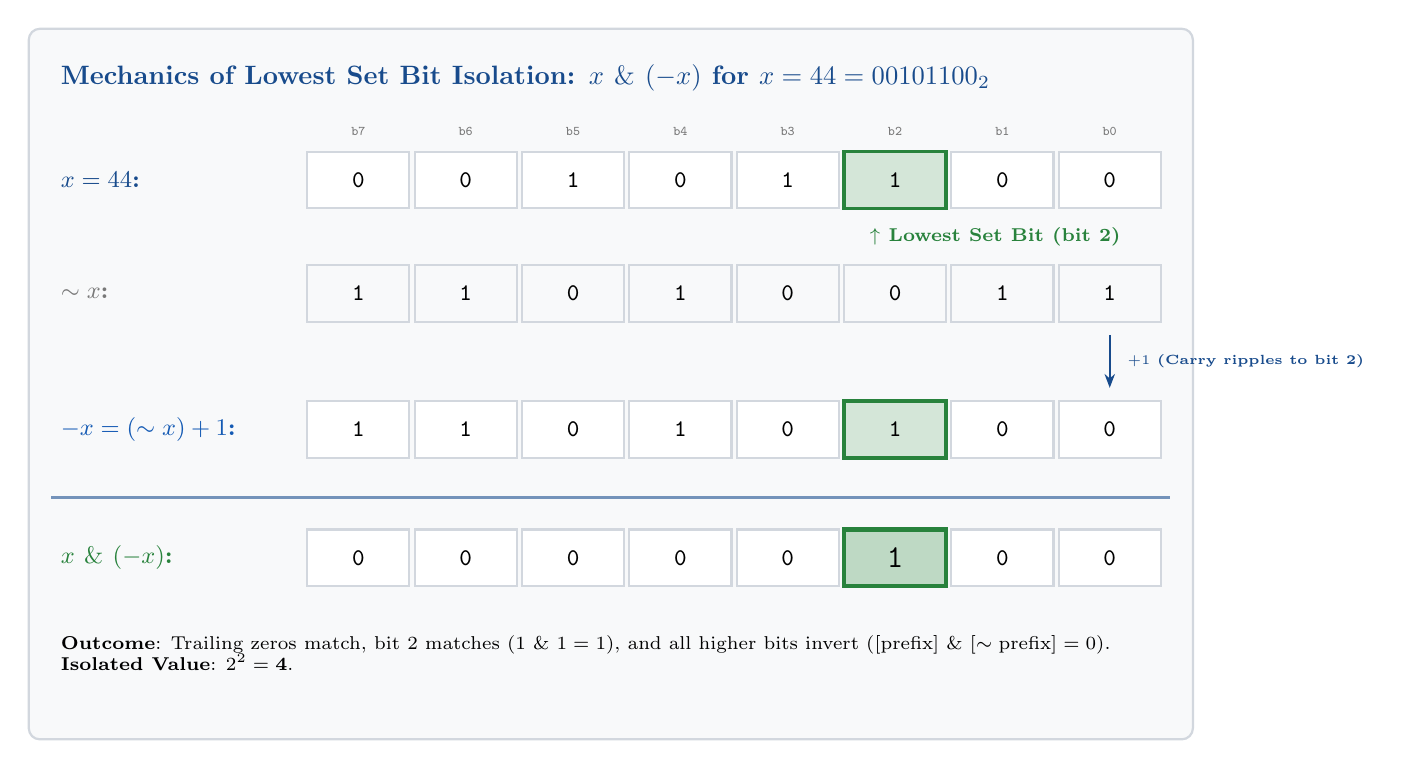
\begin{tikzpicture}[
    scale=0.96, every node/.style={transform shape},
    box/.style={draw=codeframe, fill=white, thick, minimum width=1.35cm, minimum height=0.75cm, font=\small\ttfamily, align=center},
    lbl/.style={font=\small\bfseries, align=left}
]
    % Container Frame spanning textwidth
    \draw[draw=codeframe, fill=codebg, rounded corners=4pt, thick] (0.0, -4.6) rectangle (15.4, 4.8);
    \node[anchor=north west, font=\bfseries\normalsize, text=primaryblue] at (0.3, 4.45) {Mechanics of Lowest Set Bit Isolation: $x \ \& \ (-x)$ for $x = 44 = 00101100_2$};

    % Row 1: Original x = 44
    \node[lbl, text=primaryblue, anchor=west] at (0.3, 2.8) {$x = 44$:};
    \foreach \idx/\val in {7/0, 6/0, 5/1, 4/0, 3/1, 2/1, 1/0, 0/0} {
        \pgfmathsetmacro{\xp}{14.3 - \idx * 1.42}
        \ifnum\idx=2
            \node[box, draw=codegreen, fill=codegreen!20, line width=1.3pt] (X\idx) at (\xp, 2.8) {\textbf{\val}};
        \else
            \node[box] (X\idx) at (\xp, 2.8) {\val};
        \fi
        \node[above=2pt of X\idx, font=\tiny\ttfamily, text=codegray] {b\idx};
    }
    \node[anchor=west, font=\scriptsize\bfseries, text=codegreen] at (11.0, 2.05) {$\uparrow$ Lowest Set Bit (bit 2)};

    % Row 2: Inverted ~x
    \node[lbl, text=codegray, anchor=west] at (0.3, 1.3) {$\sim x$:};
    \foreach \idx/\val in {7/1, 6/1, 5/0, 4/1, 3/0, 2/0, 1/1, 0/1} {
        \pgfmathsetmacro{\xp}{14.3 - \idx * 1.42}
        \node[box, fill=codebg] (N\idx) at (\xp, 1.3) {\val};
    }

    % Carry addition arrow
    \draw[->, thick, primaryblue, -{Stealth[length=5pt]}] (14.3, 0.75) -- (14.3, 0.05)
        node[midway, right=3pt, font=\tiny\bfseries, text=primaryblue] {$+ 1$ (Carry ripples to bit 2)};

    % Row 3: -x = (~x) + 1
    \node[lbl, text=codeblue, anchor=west] at (0.3, -0.5) {$-x = (\sim x) + 1$:};
    \foreach \idx/\val in {7/1, 6/1, 5/0, 4/1, 3/0, 2/1, 1/0, 0/0} {
        \pgfmathsetmacro{\xp}{14.3 - \idx * 1.42}
        \ifnum\idx=2
            \node[box, draw=codegreen, fill=codegreen!20, line width=1.3pt] (M\idx) at (\xp, -0.5) {\textbf{\val}};
        \else
            \node[box] (M\idx) at (\xp, -0.5) {\val};
        \fi
    }

    % Row 4: Result of AND
    \draw[draw=primaryblue!60, thick] (0.3, -1.4) -- (15.1, -1.4);
    \node[lbl, text=codegreen, anchor=west] at (0.3, -2.2) {$x \ \& \ (-x)$:};
    \foreach \idx/\val in {7/0, 6/0, 5/0, 4/0, 3/0, 2/1, 1/0, 0/0} {
        \pgfmathsetmacro{\xp}{14.3 - \idx * 1.42}
        \ifnum\idx=2
            \node[box, draw=codegreen, fill=codegreen!30, line width=1.5pt] (R\idx) at (\xp, -2.2) {\textbf{\large \val}};
        \else
            \node[box] (R\idx) at (\xp, -2.2) {\val};
        \fi
    }

    \node[anchor=north west, font=\scriptsize, align=left] at (0.3, -3.1) {
        \textbf{Outcome}: Trailing zeros match, bit 2 matches ($1 \ \& \ 1 = 1$), and all higher bits invert ($[\text{prefix}] \ \& \ [\sim\text{prefix}] = 0$).\\
        \textbf{Isolated Value}: $2^2 = \mathbf{4}$.
    };
\end{tikzpicture}}
\caption{Visual trace of lowest set bit isolation via $x \ \& \ (-x)$ on $x = 44$. Two's complement negation inverts higher-order bits while preserving the lowest set bit and trailing zeros, isolating bit 2 ($2^2 = 4$) in $O(1)$ operations.}
\end{figure}

\subsection{Diagram 27: Prefix XOR Range Query Mechanics and Self-Inverse Cancellation}

\breadcrumb{12.bit_manipulation_and_bitmasks.tex}{Section 2.6: Prefix XOR and $\mathcal{O}(1)$ Range XOR Queries}{Demonstrates self-inverse property $(X \oplus X = 0)$ annihilating prefix elements to isolate target subarray XOR in $O(1)$ operations.}

\diagramaudit{Agent (Antigravity)}{2026-10-12}{Constructed array cell trace with active target bracket; derived prefix XOR cancellation formula; recalibrated vertical card height ($5.0\text{ cm}$) and shifted array base offset to eliminate text overlap between range header and target bracket.}

\begin{figure}[htbp]
\centering
\noindent\resizebox{\textwidth}{!}{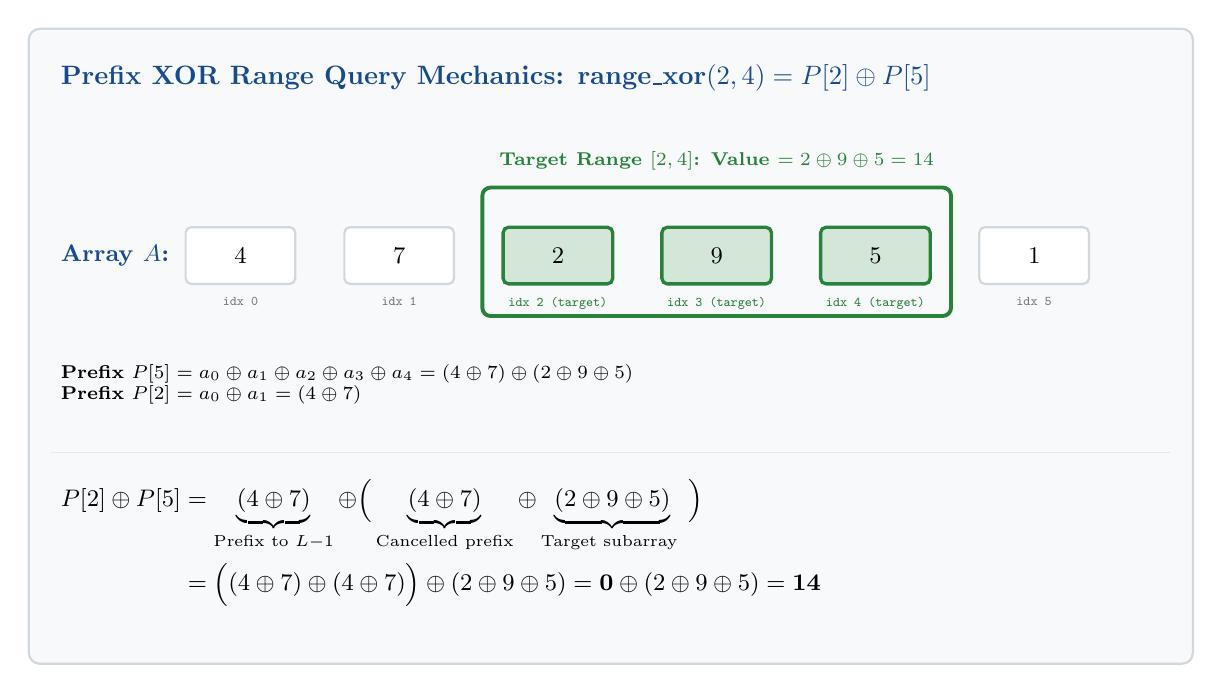
\begin{tikzpicture}[
    scale=0.96, every node/.style={transform shape},
    arrbox/.style={draw=codeframe, fill=white, thick, rounded corners=2pt, minimum width=1.45cm, minimum height=0.75cm, font=\small, align=center},
    card/.style={draw=codeframe, fill=codebg, rounded corners=4pt, thick}
]
    % Container Frame
    \draw[card] (0.0, -3.4) rectangle (15.4, 5.0);
    \node[anchor=north west, font=\bfseries\normalsize, text=primaryblue] at (0.3, 4.65) {Prefix XOR Range Query Mechanics: $\text{range\_xor}(2, 4) = P[2] \oplus P[5]$};

    % Original Array A
    \node[anchor=west, font=\small\bfseries, text=primaryblue] at (0.3, 2.0) {Array $A$:};
    \foreach \i/\val in {0/4, 1/7, 2/2, 3/9, 4/5, 5/1} {
        \pgfmathsetmacro{\cx}{2.8 + \i * 2.1}
        \ifnum\i>1\relax
            \ifnum\i<5\relax
                \node[arrbox, draw=codegreen, fill=codegreen!20, line width=1.2pt] (A\i) at (\cx, 2.0) {\val};
                \node[below=1pt of A\i, font=\tiny\ttfamily\bfseries, text=codegreen] {idx \i\ (target)};
            \else
                \node[arrbox] (A\i) at (\cx, 2.0) {\val};
                \node[below=1pt of A\i, font=\tiny\ttfamily, text=codegray] {idx \i};
            \fi
        \else
            \node[arrbox] (A\i) at (\cx, 2.0) {\val};
            \node[below=1pt of A\i, font=\tiny\ttfamily, text=codegray] {idx \i};
        \fi
    }

    % Target Range Bracket
    \draw[draw=codegreen, line width=1.4pt, rounded corners=3pt] (6.0, 1.2) rectangle (12.2, 2.9);
    \node[anchor=south, font=\scriptsize\bfseries, text=codegreen] at (9.1, 3.0) {Target Range $[2, 4]$: Value $= 2 \oplus 9 \oplus 5 = 14$};

    % Prefix Terms
    \node[anchor=west, font=\scriptsize, align=left] at (0.3, 0.3) {
        \textbf{Prefix} $P[5] = a_0 \oplus a_1 \oplus a_2 \oplus a_3 \oplus a_4 = (4 \oplus 7) \oplus (2 \oplus 9 \oplus 5)$\\
        \textbf{Prefix} $P[2] = a_0 \oplus a_1 = (4 \oplus 7)$
    };

    % XOR Equation and Cancellation
    \draw[draw=codeframe!60] (0.3, -0.6) -- (15.1, -0.6);
    \node[anchor=west, font=\small, align=left] at (0.3, -1.8) {
        $\begin{aligned}
        P[2] \oplus P[5] &= \underbrace{(4 \oplus 7)}_{\text{Prefix to } L-1} \oplus \Big( \underbrace{(4 \oplus 7)}_{\text{Cancelled prefix}} \oplus \underbrace{(2 \oplus 9 \oplus 5)}_{\text{Target subarray }} \Big) \\
        &= \Big( (4 \oplus 7) \oplus (4 \oplus 7) \Big) \oplus (2 \oplus 9 \oplus 5) = \mathbf{0} \oplus (2 \oplus 9 \oplus 5) = \mathbf{14}
        \end{aligned}$
    };
\end{tikzpicture}}
\caption{Visual cancellation in Prefix XOR range queries. Because $X \oplus X = 0$, evaluating $P[L] \oplus P[R+1]$ annihilates the preceding elements $a_0 \dots a_{L-1}$ to zero, isolating the subarray XOR sum in $O(1)$ time.}
\end{figure}

\subsection{Diagram 28: Submask Enumeration Lattice for Mask \texorpdfstring{$11 = 0b1011$}{11 = 0b1011}}

\breadcrumb{12.bit_manipulation_and_bitmasks.tex}{Section 3.2: Submask Enumeration in $\mathcal{O}(3^N)$ Time}{Visualizes descending traversal of subset lattice via \texttt{(sub - 1) \& mask}, proving avoidance of invalid non-submask states.}

\diagramaudit{Agent (Antigravity)}{2026-10-12}{Constructed 4-level subset lattice (k=3 down to k=0); verified transition arrows and descending state order; expanded card height to $4.4\text{ cm}$ to grant complete clearance between title, nodes, and generation sequence footer.}

\begin{figure}[htbp]
\centering
\noindent\resizebox{\textwidth}{!}{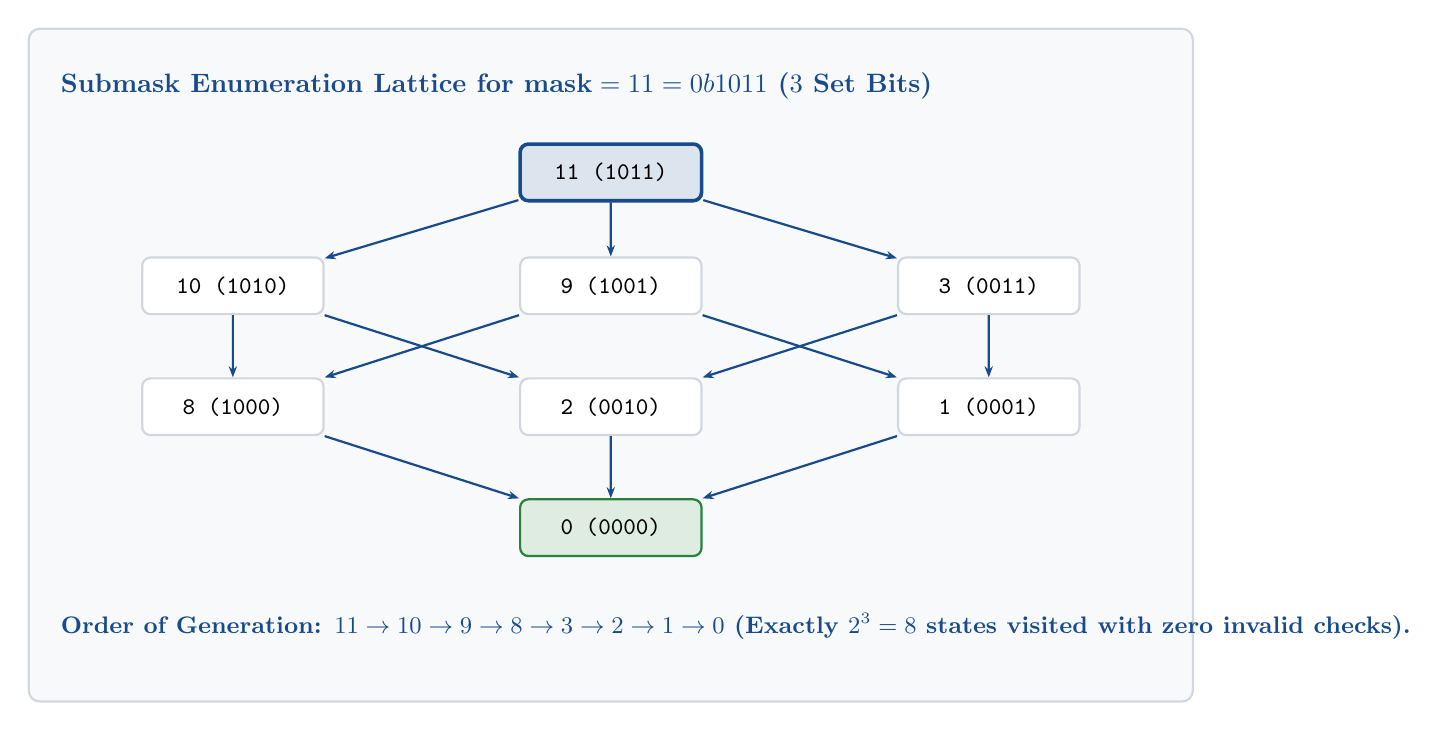
\begin{tikzpicture}[
    scale=0.96, every node/.style={transform shape},
    node distance=1.3cm and 1.8cm,
    state/.style={draw=codeframe, fill=white, thick, rounded corners=3pt, minimum width=2.4cm, minimum height=0.75cm, font=\small\ttfamily, align=center},
    arrow/.style={->, thick, primaryblue, -{Stealth[length=4pt]}}
]
    % Container Frame
    \draw[draw=codeframe, fill=codebg, rounded corners=4pt, thick] (0.0, -4.5) rectangle (15.4, 4.4);
    \node[anchor=north west, font=\bfseries\normalsize, text=primaryblue] at (0.3, 3.95) {Submask Enumeration Lattice for $\text{mask} = 11 = 0b1011$ ($3$ Set Bits)};

    % Level 3: Full Mask (k = 3)
    \node[state, draw=primaryblue, fill=primaryblue!15, line width=1.3pt] (S11) at (7.7, 2.5) {\textbf{11 (1011)}};

    % Level 2: Submasks with 2 bits set (k = 2)
    \node[state] (S10) at (2.7, 1.0) {10 (1010)};
    \node[state] (S9)  at (7.7, 1.0) {9 (1001)};
    \node[state] (S3)  at (12.7, 1.0) {3 (0011)};

    % Level 1: Submasks with 1 bit set (k = 1)
    \node[state] (S8) at (2.7, -0.6) {8 (1000)};
    \node[state] (S2) at (7.7, -0.6) {2 (0010)};
    \node[state] (S1) at (12.7, -0.6) {1 (0001)};

    % Level 0: Empty Set (k = 0)
    \node[state, draw=codegreen, fill=codegreen!15] (S0) at (7.7, -2.2) {\textbf{0 (0000)}};

    % Arrows between levels showing descending iteration sequence
    % Iteration order: 11 -> 10 -> 9 -> 8 -> 3 -> 2 -> 1 -> 0
    \draw[arrow] (S11) -- (S10);
    \draw[arrow] (S11) -- (S9);
    \draw[arrow] (S11) -- (S3);

    \draw[arrow] (S10) -- (S8);
    \draw[arrow] (S10) -- (S2);
    \draw[arrow] (S9)  -- (S8);
    \draw[arrow] (S9)  -- (S1);
    \draw[arrow] (S3)  -- (S2);
    \draw[arrow] (S3)  -- (S1);

    \draw[arrow] (S8) -- (S0);
    \draw[arrow] (S2) -- (S0);
    \draw[arrow] (S1) -- (S0);

    \node[anchor=south west, font=\small\bfseries, text=primaryblue] at (0.3, -3.8) {
        Order of Generation: $11 \to 10 \to 9 \to 8 \to 3 \to 2 \to 1 \to 0$ (Exactly $2^3 = 8$ states visited with zero invalid checks).
    };
\end{tikzpicture}}
\caption{The submask lattice for $\text{mask} = 11$ ($0b1011_2$). The expression \texttt{sub = (sub - 1) \& mask} transitions strictly between valid subset states, bypassing all non-submask integers and achieving $O(3^N)$ global enumeration.}
\end{figure}


\newpage
% ============================================================================
\newpage
\section{Module 09: String Algorithms}
\newpage
% ============================================================================
\newpage

\subsection{Diagram 29: Trie (Prefix Tree) Multi-Word Search \& Vector Pool Memory Layout}

\breadcrumb{09.string_algorithms.tex}{Section 2.3: Tries (Prefix Trees)}{Demystifies character branching, terminal word markers, prefix sharing, and cache-friendly vector node pool allocation.}

\diagramaudit{Agent (Antigravity)}{2026-10-12}{Constructed full-width dual-panel layout: left tree graph visualizes shared prefixes across car, cat, cart, dog, dot with double-bordered terminal nodes; right panel details vector pool indexing and O(L) traversal mechanics.}

\begin{figure}[htbp]
\centering
\noindent\resizebox{\textwidth}{!}{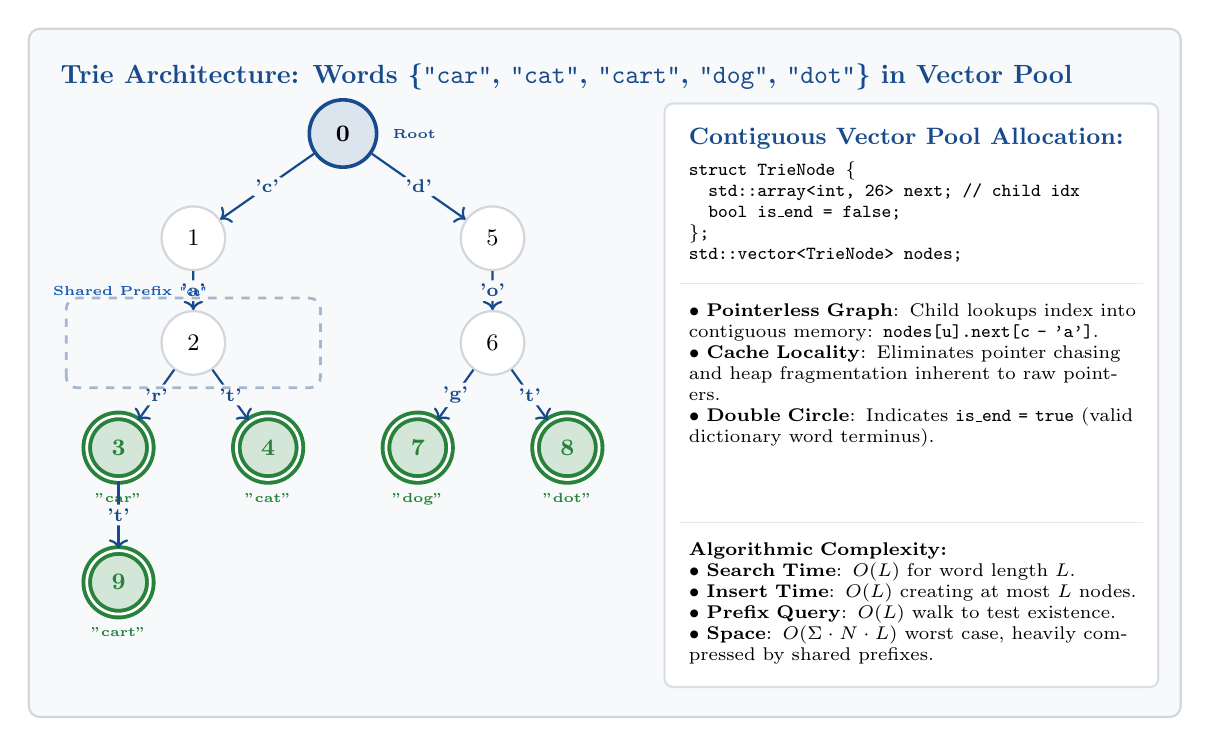
\begin{tikzpicture}[
    scale=0.95, every node/.style={transform shape},
    troot/.style={circle, draw=primaryblue, fill=primaryblue!15, line width=1.3pt, minimum size=0.9cm, font=\small\bfseries, align=center},
    tnode/.style={circle, draw=codeframe, fill=white, thick, minimum size=0.85cm, font=\small, align=center},
    tend/.style={circle, draw=codegreen, fill=codegreen!20, line width=1.4pt, double, double distance=1pt, minimum size=0.85cm, font=\small\bfseries, text=codegreen, align=center},
    edgeLbl/.style={font=\scriptsize\bfseries, text=primaryblue, fill=codebg, inner sep=1.5pt, rounded corners=2pt},
    card/.style={draw=codeframe, fill=codebg, rounded corners=4pt, thick}
]
    % Container Frame
    \draw[card] (0.0, -4.2) rectangle (15.4, 5.0);
    \node[anchor=north west, font=\bfseries\normalsize, text=primaryblue] at (0.3, 4.65) {Trie Architecture: Words \{\texttt{"car"}, \texttt{"cat"}, \texttt{"cart"}, \texttt{"dog"}, \texttt{"dot"}\} in Vector Pool};

    % --- Left Panel: Tree Graph (x: 0.2 to 8.2) ---
    % Root
    \node[troot] (R) at (4.2, 3.6) {0};
    \node[right=2pt of R, font=\tiny\bfseries, text=primaryblue] {Root};

    % Level 1: 'c' and 'd'
    \node[tnode] (C) at (2.2, 2.2) {1};
    \node[tnode] (D) at (6.2, 2.2) {5};

    \draw[->, thick, primaryblue] (R) -- (C) node[midway, edgeLbl] {'c'};
    \draw[->, thick, primaryblue] (R) -- (D) node[midway, edgeLbl] {'d'};

    % Level 2: 'a' under 'c', 'o' under 'd'
    \node[tnode] (A) at (2.2, 0.8) {2};
    \node[tnode] (O) at (6.2, 0.8) {6};

    \draw[->, thick, primaryblue] (C) -- (A) node[midway, edgeLbl] {'a'};
    \draw[->, thick, primaryblue] (D) -- (O) node[midway, edgeLbl] {'o'};

    % Level 3: under 'a' -> 'r' and 't'; under 'o' -> 'g' and 't'
    \node[tend] (R3) at (1.2, -0.6) {3};
    \node[tend] (T4) at (3.2, -0.6) {4};
    \node[tend] (G7) at (5.2, -0.6) {7};
    \node[tend] (T8) at (7.2, -0.6) {8};

    \draw[->, thick, primaryblue] (A) -- (R3) node[midway, edgeLbl] {'r'};
    \draw[->, thick, primaryblue] (A) -- (T4) node[midway, edgeLbl] {'t'};
    \draw[->, thick, primaryblue] (O) -- (G7) node[midway, edgeLbl] {'g'};
    \draw[->, thick, primaryblue] (O) -- (T8) node[midway, edgeLbl] {'t'};

    \node[below=1pt of R3, font=\tiny\bfseries, text=codegreen] {"car"};
    \node[below=1pt of T4, font=\tiny\bfseries, text=codegreen] {"cat"};
    \node[below=1pt of G7, font=\tiny\bfseries, text=codegreen] {"dog"};
    \node[below=1pt of T8, font=\tiny\bfseries, text=codegreen] {"dot"};

    % Level 4: under 'r' -> 't' for "cart"
    \node[tend] (T9) at (1.2, -2.4) {9};
    \draw[->, thick, primaryblue] (R3) -- (T9) node[midway, edgeLbl] {'t'};
    \node[below=1pt of T9, font=\tiny\bfseries, text=codegreen] {"cart"};

    % Common prefix highlight
    \draw[draw=primaryblue!40, dashed, rounded corners=4pt, line width=1pt] (0.5, 0.2) rectangle (3.9, 1.4);
    \node[anchor=west, font=\tiny\bfseries, text=codeblue] at (0.2, 1.5) {Shared Prefix \texttt{"ca"}};

    % --- Right Panel: Memory Model & Mechanics (x: 8.5 to 15.1) ---
    \draw[draw=codeframe!80, fill=white, rounded corners=3pt, thick] (8.5, -3.8) rectangle (15.1, 4.0);
    \node[anchor=north west, font=\small\bfseries, text=primaryblue] at (8.7, 3.8) {Contiguous Vector Pool Allocation:};

    \node[anchor=north west, font=\scriptsize\ttfamily, text=black, align=left] at (8.7, 3.35) {
        \textbf{struct} TrieNode \{\\
        \phantom{x} \textbf{std::array}<int, 26> next; // child idx\\
        \phantom{x} \textbf{bool} is\_end = false;\\
        \};\\
        \textbf{std::vector}<TrieNode> nodes;
    };

    \draw[draw=codeframe!60] (8.7, 1.6) -- (14.9, 1.6);

    \node[anchor=north west, font=\scriptsize, align=left, text width=6.0cm] at (8.7, 1.45) {
        $\bullet$ \textbf{Pointerless Graph}: Child lookups index into contiguous memory: \texttt{nodes[u].next[c - 'a']}.\\
        $\bullet$ \textbf{Cache Locality}: Eliminates pointer chasing and heap fragmentation inherent to raw pointers.\\
        $\bullet$ \textbf{Double Circle}: Indicates \texttt{is\_end = true} (valid dictionary word terminus).
    };

    \draw[draw=codeframe!60] (8.7, -1.6) -- (14.9, -1.6);

    \node[anchor=north west, font=\scriptsize, align=left, text width=6.0cm] at (8.7, -1.75) {
        \textbf{Algorithmic Complexity:}\\
        $\bullet$ \textbf{Search Time}: $O(L)$ for word length $L$.\\
        $\bullet$ \textbf{Insert Time}: $O(L)$ creating at most $L$ nodes.\\
        $\bullet$ \textbf{Prefix Query}: $O(L)$ walk to test existence.\\
        $\bullet$ \textbf{Space}: $O(\Sigma \cdot N \cdot L)$ worst case, heavily compressed by shared prefixes.
    };
\end{tikzpicture}}
\caption{Trie architecture and memory model. Shared prefixes (\texttt{"ca"}, \texttt{"do"}) branch through a contiguous node pool, reducing search and prefix verification to $O(L)$ operations independent of total dictionary size.}
\end{figure}

\newpage
\newpage
\newpage

\subsection{Diagram 30: KMP Prefix Function (\texorpdfstring{$\pi$}{pi}) \& Failure Table Fallback Transitions}

\breadcrumb{09.string_algorithms.tex}{Section 2.2: The KMP Algorithm and Prefix Function}{Visualizes longest proper prefix/suffix matching values in the $\pi$ table and the zero-backtracking text pointer fallback jump.}

\diagramaudit{Agent (Antigravity)}{2026-10-12}{Constructed full-width 3-stage visual trace: top array displays pattern P = "ABABC"; middle table breaks down proper prefix vs suffix matches; bottom alignment trace details non-backtracking text pointer transition when mismatch occurs at P[4].}

\begin{figure}[htbp]
\centering
\noindent\resizebox{\textwidth}{!}{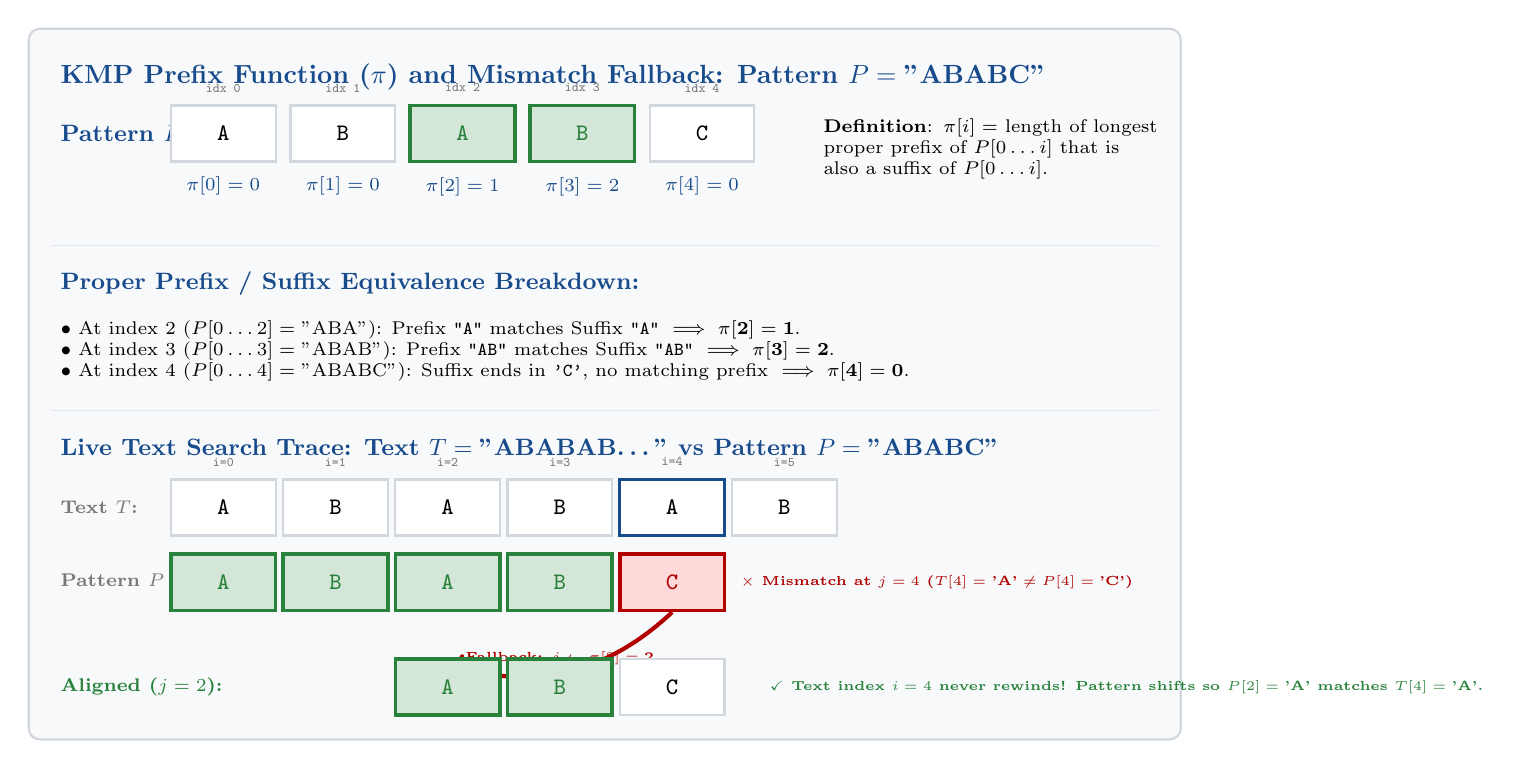
\begin{tikzpicture}[
    scale=0.95, every node/.style={transform shape},
    cell/.style={draw=codeframe, fill=white, thick, minimum width=1.4cm, minimum height=0.75cm, font=\small\ttfamily, align=center},
    matchcell/.style={draw=codegreen, fill=codegreen!20, line width=1.3pt, minimum width=1.4cm, minimum height=0.75cm, font=\small\ttfamily\bfseries, text=codegreen, align=center},
    failcell/.style={draw=red!70!black, fill=red!15, line width=1.3pt, minimum width=1.4cm, minimum height=0.75cm, font=\small\ttfamily\bfseries, text=red!70!black, align=center},
    card/.style={draw=codeframe, fill=codebg, rounded corners=4pt, thick}
]
    % Container Frame
    \draw[card] (0.0, -4.5) rectangle (15.4, 5.0);
    \node[anchor=north west, font=\bfseries\normalsize, text=primaryblue] at (0.3, 4.65) {KMP Prefix Function ($\pi$) and Mismatch Fallback: Pattern $P = \text{"ABABC"}$};

    % --- Top Panel: Pattern P and Pi Array (x: 0.3 to 15.1, y: 3.8 to 2.0) ---
    \node[anchor=west, font=\small\bfseries, text=primaryblue] at (0.3, 3.6) {Pattern $P$:};
    \foreach \idx/\ch/\pival in {0/A/0, 1/B/0, 2/A/1, 3/B/2, 4/C/0} {
        \pgfmathsetmacro{\cx}{2.6 + \idx * 1.6}
        \ifnum\pival>0
            \node[matchcell] (P\idx) at (\cx, 3.6) {\ch};
        \else
            \node[cell] (P\idx) at (\cx, 3.6) {\ch};
        \fi
        \node[above=1pt of P\idx, font=\tiny\ttfamily, text=codegray] {idx \idx};
        \node[below=2pt of P\idx, font=\scriptsize\bfseries, text=primaryblue] {$\pi[\idx] = \pival$};
    }

    % Summary explanation of Pi
    \node[anchor=west, font=\scriptsize, align=left, text width=4.5cm] at (10.5, 3.4) {
        \textbf{Definition}: $\pi[i] =$ length of longest proper prefix of $P[0 \dots i]$ that is also a suffix of $P[0 \dots i]$.
    };

    % --- Middle Panel: Prefix vs Suffix Equivalence (y: 1.4 to 0.0) ---
    \draw[draw=codeframe!60] (0.3, 2.1) -- (15.1, 2.1);
    \node[anchor=west, font=\small\bfseries, text=primaryblue] at (0.3, 1.6) {Proper Prefix / Suffix Equivalence Breakdown:};

    \node[anchor=west, font=\scriptsize, align=left] at (0.3, 0.7) {
        $\bullet$ At index $2$ ($P[0\dots 2] = \text{"ABA"} $): Prefix \texttt{"A"} matches Suffix \texttt{"A"} $\implies \mathbf{\pi[2] = 1}$.\\
        $\bullet$ At index $3$ ($P[0\dots 3] = \text{"ABAB"} $): Prefix \texttt{"AB"} matches Suffix \texttt{"AB"} $\implies \mathbf{\pi[3] = 2}$.\\
        $\bullet$ At index $4$ ($P[0\dots 4] = \text{"ABABC"} $): Suffix ends in \texttt{'C'}, no matching prefix $\implies \mathbf{\pi[4] = 0}$.
    };

    % --- Bottom Panel: Mismatch Fallback Trace (y: -0.2 to -4.1) ---
    \draw[draw=codeframe!60] (0.3, -0.1) -- (15.1, -0.1);
    \node[anchor=west, font=\small\bfseries, text=primaryblue] at (0.3, -0.6) {Live Text Search Trace: Text $T = \text{"ABABAB\dots"}$ vs Pattern $P = \text{"ABABC"}$};

    % Text T cells
    \node[anchor=west, font=\scriptsize\bfseries, text=codegray] at (0.3, -1.4) {Text $T$:};
    \foreach \idx/\ch in {0/A, 1/B, 2/A, 3/B, 4/A, 5/B} {
        \pgfmathsetmacro{\cx}{2.6 + \idx * 1.5}
        \ifnum\idx=4
            \node[cell, draw=primaryblue, line width=1.2pt] (T\idx) at (\cx, -1.4) {\textbf{\ch}};
        \else
            \node[cell] (T\idx) at (\cx, -1.4) {\ch};
        \fi
        \node[above=1pt of T\idx, font=\tiny\ttfamily, text=codegray] {i=\idx};
    }

    % Pattern P before mismatch
    \node[anchor=west, font=\scriptsize\bfseries, text=codegray] at (0.3, -2.4) {Pattern $P$ (j):};
    \foreach \idx/\ch in {0/A, 1/B, 2/A, 3/B, 4/C} {
        \pgfmathsetmacro{\cx}{2.6 + \idx * 1.5}
        \ifnum\idx=4
            \node[failcell] (Pj\idx) at (\cx, -2.4) {\ch};
        \else
            \node[matchcell] (Pj\idx) at (\cx, -2.4) {\ch};
        \fi
    }
    \node[right=2pt of Pj4, font=\tiny\bfseries, text=red!70!black] {$\times$ Mismatch at $j=4$ ($T[4]=\text{'A'} \ne P[4]=\text{'C'}$)};

    % Fallback Jump Arrow
    \draw[->, line width=1.5pt, red!70!black] (8.6, -2.8) to[bend left=30] (5.6, -3.5);
    \node[anchor=north, font=\tiny\bfseries, text=red!70!black] at (7.1, -3.2) {Fallback: $j \leftarrow \pi[3] = \mathbf{2}$};

    % Aligned Pattern after jump
    \node[anchor=west, font=\scriptsize\bfseries, text=codegreen] at (0.3, -3.8) {Aligned ($j=2$):};
    \node[matchcell] at (5.6, -3.8) {A};
    \node[matchcell] at (7.1, -3.8) {B};
    \node[cell] at (8.6, -3.8) {C};
    \node[right=5pt of Pj4, font=\tiny\bfseries, text=codegreen, anchor=west] at (9.6, -3.8) {
        $\checkmark$ Text index $i=4$ never rewinds! Pattern shifts so $P[2]=\text{'A'}$ matches $T[4]=\text{'A'}$.
    };
\end{tikzpicture}}
\caption{KMP prefix function ($\pi$) and non-backtracking fallback transition. When character mismatch occurs at index $j = 4$, the pattern pointer jumps immediately to $\pi[j-1] = \pi[3] = 2$, preserving the matching prefix \texttt{"AB"} without rewinding the text pointer $i$.}
\end{figure}

\newpage
\newpage
\newpage

\subsection{Diagram 31: Rabin-Karp Polynomial Rolling Hash Window Shift \& Arithmetic Mechanics}

\breadcrumb{09.string_algorithms.tex}{Section 3.2: Sliding Window Substring Search (Rabin-Karp)}{Visualizes O(1) rolling hash window transitions by decomposing high-order character eviction, base multiplication shift, and low-order ingestion.}

\diagramaudit{Agent (Antigravity)}{2026-10-12}{Established full-width multi-tier layout: top text tape tracks window shift W1 = "abc" -> W2 = "bcd"; middle panel breaks down 3-step modulo polynomial transformation; bottom card details double-hash collision prevention.}

\begin{figure}[htbp]
\centering
\noindent\resizebox{\textwidth}{!}{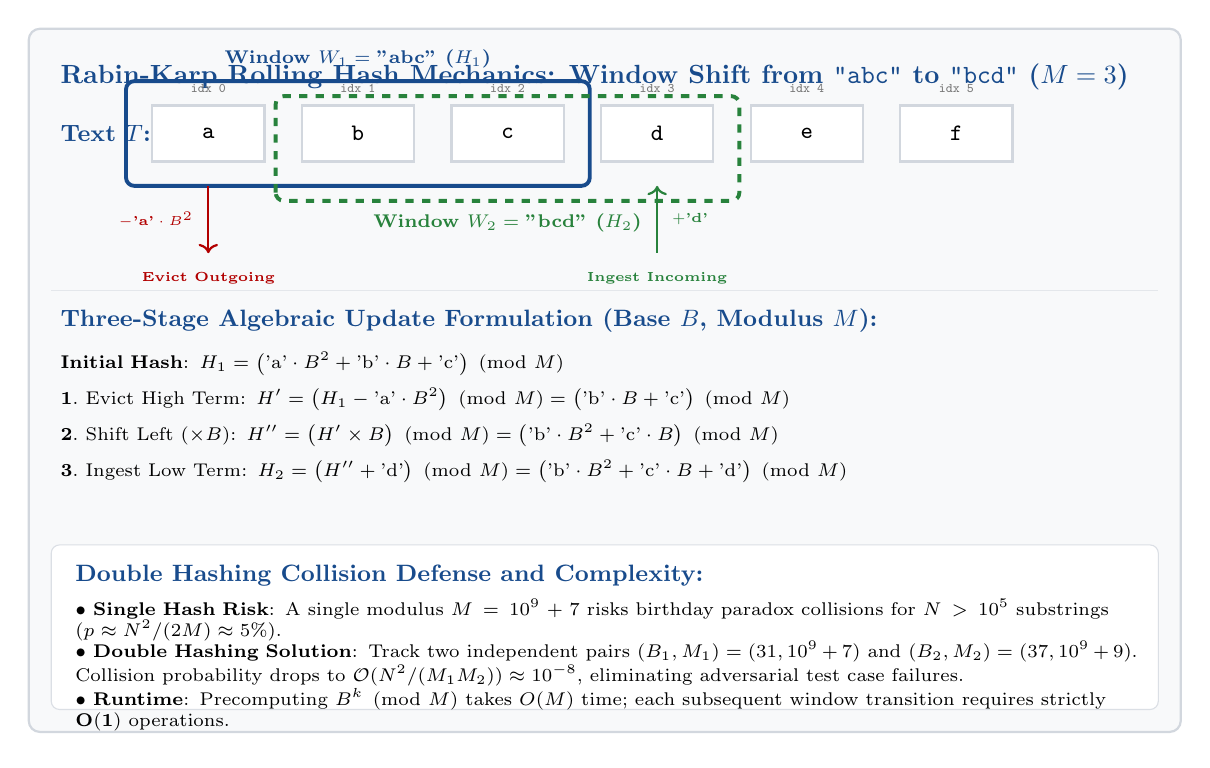
\begin{tikzpicture}[
    scale=0.95, every node/.style={transform shape},
    tapebox/.style={draw=codeframe, fill=white, thick, minimum width=1.5cm, minimum height=0.75cm, font=\small\ttfamily, align=center},
    card/.style={draw=codeframe, fill=codebg, rounded corners=4pt, thick}
]
    % Container Frame
    \draw[card] (0.0, -4.6) rectangle (15.4, 4.8);
    \node[anchor=north west, font=\bfseries\normalsize, text=primaryblue] at (0.3, 4.45) {Rabin-Karp Rolling Hash Mechanics: Window Shift from \texttt{"abc"} to \texttt{"bcd"} ($M=3$)};

    % --- Top Panel: Text Tape (y: 3.5 to 2.2) ---
    \node[anchor=west, font=\small\bfseries, text=primaryblue] at (0.3, 3.4) {Text $T$:};
    \foreach \idx/\ch in {0/a, 1/b, 2/c, 3/d, 4/e, 5/f} {
        \pgfmathsetmacro{\cx}{2.4 + \idx * 2.0}
        \node[tapebox] (C\idx) at (\cx, 3.4) {\textbf{\ch}};
        \node[above=1pt of C\idx, font=\tiny\ttfamily, text=codegray] {idx \idx};
    }

    % Window W1 frame [0..2]
    \draw[draw=primaryblue, line width=1.4pt, rounded corners=3pt] (1.3, 2.7) rectangle (7.5, 4.1);
    \node[anchor=south, font=\scriptsize\bfseries, text=primaryblue] at (4.4, 4.15) {Window $W_1 = \text{"abc"}$ ($H_1$)};

    % Window W2 frame [1..3]
    \draw[draw=codegreen, line width=1.4pt, dashed, rounded corners=3pt] (3.3, 2.5) rectangle (9.5, 3.9);
    \node[anchor=north, font=\scriptsize\bfseries, text=codegreen] at (6.4, 2.45) {Window $W_2 = \text{"bcd"}$ ($H_2$)};

    % Eviction & Ingestion Annotations
    \draw[->, thick, red!70!black] (2.4, 2.7) -- (2.4, 1.8) node[midway, left=2pt, font=\tiny\bfseries] {$- \text{'a'} \cdot B^2$};
    \node[below=1pt, font=\tiny\bfseries, text=red!70!black] at (2.4, 1.7) {Evict Outgoing};

    \draw[<-, thick, codegreen] (8.4, 2.7) -- (8.4, 1.8) node[midway, right=2pt, font=\tiny\bfseries] {$+ \text{'d'}$};
    \node[below=1pt, font=\tiny\bfseries, text=codegreen] at (8.4, 1.7) {Ingest Incoming};

    % --- Middle Panel: Mathematical 3-Stage Transition (y: 1.2 to -2.0) ---
    \draw[draw=codeframe!60] (0.3, 1.3) -- (15.1, 1.3);
    \node[anchor=west, font=\small\bfseries, text=primaryblue] at (0.3, 0.9) {Three-Stage Algebraic Update Formulation (Base $B$, Modulus $M$):};

    \node[anchor=west, font=\scriptsize, align=left, text width=14.5cm] at (0.3, -0.4) {
        \textbf{Initial Hash}: $H_1 = \big( \text{'a'} \cdot B^2 + \text{'b'} \cdot B + \text{'c'} \big) \pmod M$\\[4pt]
        $\mathbf{1.\ \text{Evict High Term}}$: $H' = \big( H_1 - \text{'a'} \cdot B^2 \big) \pmod M = \big( \text{'b'} \cdot B + \text{'c'} \big) \pmod M$\\[4pt]
        $\mathbf{2.\ \text{Shift Left}}\ (\times B)$: $H'' = \big( H' \times B \big) \pmod M = \big( \text{'b'} \cdot B^2 + \text{'c'} \cdot B \big) \pmod M$\\[4pt]
        $\mathbf{3.\ \text{Ingest Low Term}}$: $H_2 = \big( H'' + \text{'d'} \big) \pmod M = \big( \text{'b'} \cdot B^2 + \text{'c'} \cdot B + \text{'d'} \big) \pmod M$
    };

    % --- Bottom Card: Collision Defense & Complexity (y: -2.2 to -4.3) ---
    \draw[draw=codeframe!80, fill=white, rounded corners=3pt] (0.3, -4.3) rectangle (15.1, -2.1);
    \node[anchor=north west, font=\small\bfseries, text=primaryblue] at (0.5, -2.25) {Double Hashing Collision Defense and Complexity:};

    \node[anchor=north west, font=\scriptsize, align=left, text width=14.2cm] at (0.5, -2.7) {
        $\bullet$ \textbf{Single Hash Risk}: A single modulus $M = 10^9+7$ risks birthday paradox collisions for $N > 10^5$ substrings ($p \approx N^2 / (2M) \approx 5\%$).\\
        $\bullet$ \textbf{Double Hashing Solution}: Track two independent pairs $(B_1, M_1) = (31, 10^9+7)$ and $(B_2, M_2) = (37, 10^9+9)$. Collision probability drops to $\mathcal{O}(N^2 / (M_1 M_2)) \approx 10^{-8}$, eliminating adversarial test case failures.\\
        $\bullet$ \textbf{Runtime}: Precomputing $B^k \pmod M$ takes $O(M)$ time; each subsequent window transition requires strictly $\mathbf{O(1)}$ operations.
    };
\end{tikzpicture}}
\caption{Rabin-Karp polynomial rolling hash window slide mechanics. By subtracting the outgoing character's high-order power $c_{\text{out}} \cdot B^{M-1}$, multiplying by base $B$, and adding the incoming character $c_{\text{in}}$, the new window hash is computed in $O(1)$ operations.}
\end{figure}

\newpage
\newpage
\newpage
% ============================================================================
\newpage
\section{Monograph Visual Expansions: Core Algorithmic Paradigms}
\newpage
% ============================================================================
\newpage

\subsection[Diagram 32: 2D Prefix Sum Subgrid Range Query]{Diagram 32: 2D Prefix Sum Range Query via Inclusion-Exclusion}

\breadcrumb{04.sequences_and_series.tex}{Section 5: 2D Matrix Block Sum: Range Queries in a Grid}{Visualizes geometric submatrix decomposition into four overlapping regions (A, B, C, D) and explains why the top-left corner is added back.}

\diagramaudit{Agent (Antigravity)}{2026-10-12}{Constructed full-width 2-panel layout: left coordinate matrix dissects 4 subgrid zones A, B, C, D; right panel details the algebraic inclusion-exclusion cancellation and 1-based index padding invariants.}

\begin{figure}[htbp]
\centering
\noindent\resizebox{0.99\textwidth}{!}{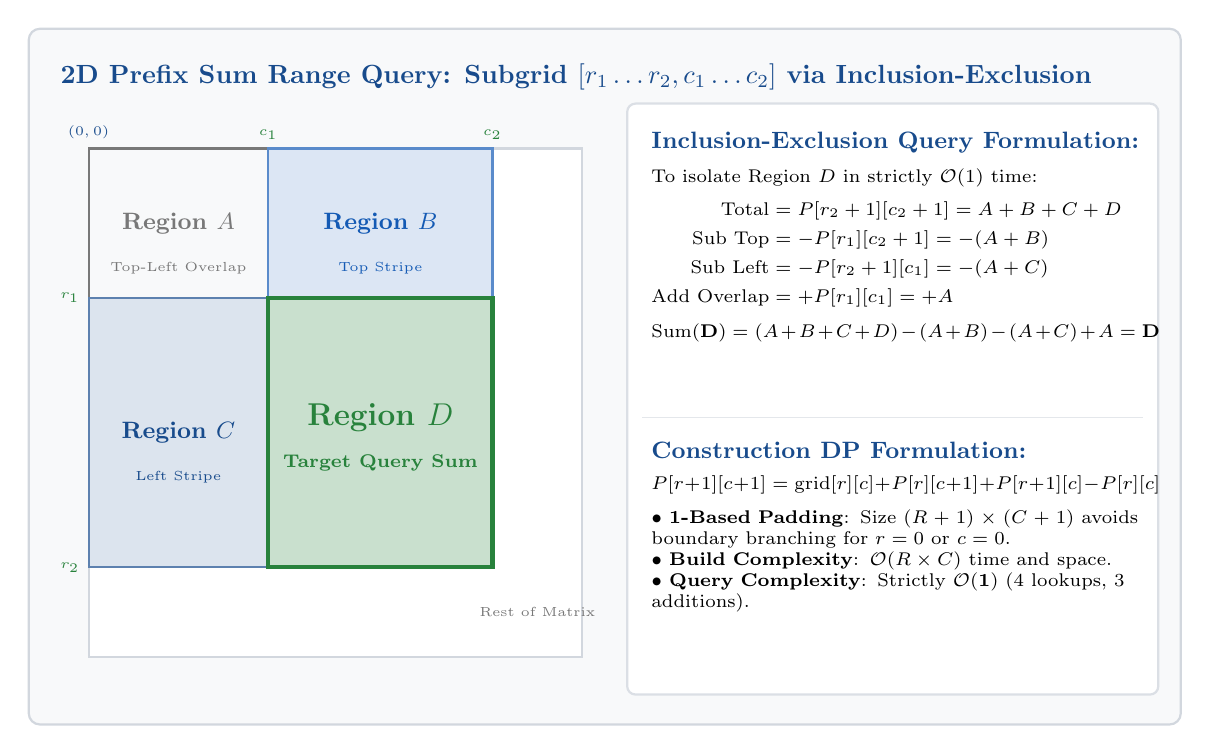
\begin{tikzpicture}[
    scale=0.95, every node/.style={transform shape},
    card/.style={draw=codeframe, fill=codebg, rounded corners=4pt, thick}
]
    % Container Frame
    \draw[card] (0.0, -4.5) rectangle (15.4, 4.8);
    \node[anchor=north west, font=\bfseries\normalsize, text=primaryblue] at (0.3, 4.45) {2D Prefix Sum Range Query: Subgrid $[r_1 \dots r_2, c_1 \dots c_2]$ via Inclusion-Exclusion};

    % --- Left Panel: Matrix Subregions (x: 0.3 to 7.8, y: 3.6 to -4.0) ---
    % Grid background
    \draw[draw=codeframe, fill=white, thick] (0.8, -3.6) rectangle (7.4, 3.2);

    % Region A (Top-Left corner: rows 0..r1-1, cols 0..c1-1)
    \draw[draw=codegray, fill=codebg, thick] (0.8, 1.2) rectangle (3.2, 3.2);
    \node[font=\small\bfseries, text=codegray] at (2.0, 2.2) {Region $A$};
    \node[font=\tiny, text=codegray] at (2.0, 1.6) {Top-Left Overlap};

    % Region B (Top stripe: rows 0..r1-1, cols c1..c2)
    \draw[draw=codeblue!70, fill=codeblue!15, thick] (3.2, 1.2) rectangle (6.2, 3.2);
    \node[font=\small\bfseries, text=codeblue] at (4.7, 2.2) {Region $B$};
    \node[font=\tiny, text=codeblue] at (4.7, 1.6) {Top Stripe};

    % Region C (Left stripe: rows r1..r2, cols 0..c1-1)
    \draw[draw=primaryblue!70, fill=primaryblue!15, thick] (0.8, -2.4) rectangle (3.2, 1.2);
    \node[font=\small\bfseries, text=primaryblue] at (2.0, -0.6) {Region $C$};
    \node[font=\tiny, text=primaryblue] at (2.0, -1.2) {Left Stripe};

    % Region D (Target Subgrid: rows r1..r2, cols c1..c2)
    \draw[draw=codegreen, fill=codegreen!25, line width=1.5pt] (3.2, -2.4) rectangle (6.2, 1.2);
    \node[font=\large\bfseries, text=codegreen] at (4.7, -0.4) {Region $D$};
    \node[font=\scriptsize\bfseries, text=codegreen] at (4.7, -1.0) {Target Query Sum};

    % Exterior area (outside query)
    \node[font=\tiny, text=codegray] at (6.8, -3.0) {Rest of Matrix};

    % Coordinate ticks and labels
    \node[above, font=\tiny\ttfamily, text=primaryblue] at (0.8, 3.2) {$(0,0)$};
    \node[above, font=\tiny\ttfamily, text=codegreen] at (3.2, 3.2) {$c_1$};
    \node[above, font=\tiny\ttfamily, text=codegreen] at (6.2, 3.2) {$c_2$};
    \node[left, font=\tiny\ttfamily, text=codegreen] at (0.8, 1.2) {$r_1$};
    \node[left, font=\tiny\ttfamily, text=codegreen] at (0.8, -2.4) {$r_2$};

    % --- Right Panel: Mathematical Formulations (x: 8.0 to 15.1) ---
    \draw[draw=codeframe!80, fill=white, rounded corners=3pt, thick] (8.0, -4.1) rectangle (15.1, 3.8);
    \node[anchor=north west, font=\small\bfseries, text=primaryblue] at (8.2, 3.55) {Inclusion-Exclusion Query Formulation:};

    \node[anchor=north west, font=\scriptsize, align=left, text width=6.8cm] at (8.2, 3.05) {
        To isolate Region $D$ in strictly $\mathcal{O}(1)$ time:\\[4pt]
        $\begin{aligned}
        \text{Total} &= P[r_2+1][c_2+1] = A + B + C + D\\
        \text{Sub Top} &= - P[r_1][c_2+1] = -(A + B)\\
        \text{Sub Left} &= - P[r_2+1][c_1] = -(A + C)\\
        \text{Add Overlap} &= + P[r_1][c_1] = + A
        \end{aligned}$\\[5pt]
        $\mathbf{\text{Sum}(D)} = (A+B+C+D) - (A+B) - (A+C) + A = \mathbf{D}$
    };

    \draw[draw=codeframe!60] (8.2, -0.4) -- (14.9, -0.4);

    \node[anchor=north west, font=\small\bfseries, text=primaryblue] at (8.2, -0.6) {Construction DP Formulation:};
    \node[anchor=north west, font=\scriptsize, align=left, text width=6.8cm] at (8.2, -1.05) {
        $P[r+1][c+1] = \text{grid}[r][c] + P[r][c+1] + P[r+1][c] - P[r][c]$\\[5pt]
        $\bullet$ \textbf{1-Based Padding}: Size $(R+1) \times (C+1)$ avoids boundary branching for $r=0$ or $c=0$.\\
        $\bullet$ \textbf{Build Complexity}: $\mathcal{O}(R \times C)$ time and space.\\
        $\bullet$ \textbf{Query Complexity}: Strictly $\mathbf{\mathcal{O}(1)}$ (4 lookups, 3 additions).
    };
\end{tikzpicture}}%
\caption{2D prefix sum subgrid range query via the inclusion-exclusion principle. Isolating rectangular subgrid $D$ subtracts the bounding rectangles above and left, and adds back the doubly subtracted top-left region $A$ in $O(1)$ operations.}
\end{figure}

\newpage
\newpage
\newpage

\subsection[Diagram 33: 0/1 Knapsack Decision Grid]{Diagram 33: 0/1 Knapsack Decision Grid \& 1D Space-Optimized Reverse Traverse}

\breadcrumb{06.dynamic_programming.tex}{Section 2.7: The Knapsack Family}{Visualizes 2D subproblem dependencies (skip vs take) and proves why the 1D space-optimized array MUST iterate backwards.}

\diagramaudit{Agent (Antigravity)}{2026-10-12}{Constructed full-width comparative architecture: left grid maps 2D skip/take state dependency arrows; right panel contrasts forward iteration corruption (unbounded knapsack) against safe reverse traversal (0/1 enforcement in O(W) space).}

\begin{figure}[htbp]
\centering
\noindent\resizebox{\textwidth}{!}{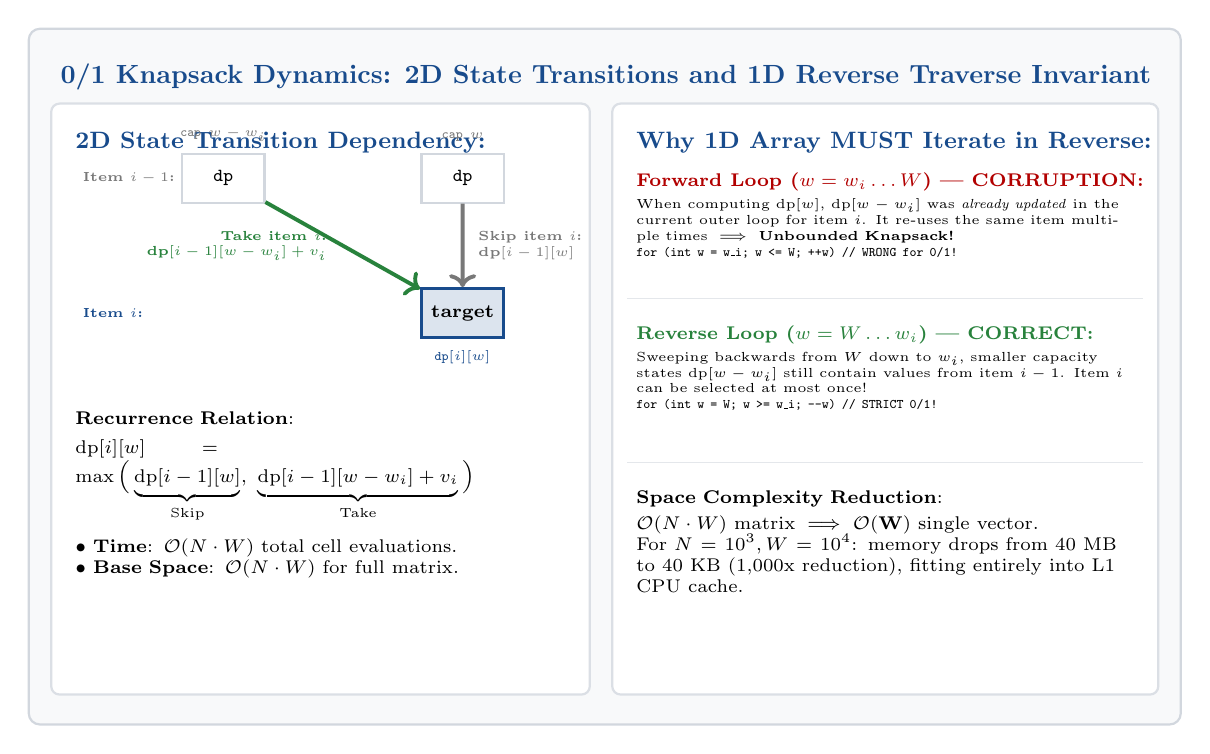
\begin{tikzpicture}[
    scale=0.95, every node/.style={transform shape},
    cell/.style={draw=codeframe, fill=white, thick, minimum width=1.1cm, minimum height=0.65cm, font=\scriptsize\ttfamily, align=center},
    hiCell/.style={draw=primaryblue, fill=primaryblue!15, line width=1.2pt, minimum width=1.1cm, minimum height=0.65cm, font=\scriptsize\bfseries, align=center},
    card/.style={draw=codeframe, fill=codebg, rounded corners=4pt, thick}
]
    % Container Frame
    \draw[card] (0.0, -4.5) rectangle (15.4, 4.8);
    \node[anchor=north west, font=\bfseries\normalsize, text=primaryblue] at (0.3, 4.45) {0/1 Knapsack Dynamics: 2D State Transitions and 1D Reverse Traverse Invariant};

    % --- Left Panel: 2D Dependency Lattice (x: 0.3 to 7.6) ---
    \draw[draw=codeframe!80, fill=white, rounded corners=3pt, thick] (0.3, -4.1) rectangle (7.5, 3.8);
    \node[anchor=north west, font=\small\bfseries, text=primaryblue] at (0.5, 3.55) {2D State Transition Dependency:};

    % Table grid for items vs capacities
    \node[anchor=west, font=\tiny\bfseries, text=codegray] at (0.6, 2.8) {Item $i-1$:};
    \node[cell] (PrevW) at (5.8, 2.8) {dp};
    \node[above=1pt of PrevW, font=\tiny\ttfamily, text=codegray] {cap $w$};

    \node[cell] (PrevSub) at (2.6, 2.8) {dp};
    \node[above=1pt of PrevSub, font=\tiny\ttfamily, text=codegray] {cap $w - w_i$};

    \node[anchor=west, font=\tiny\bfseries, text=primaryblue] at (0.6, 1.0) {Item $i$:};
    \node[hiCell] (CurrW) at (5.8, 1.0) {target};
    \node[below=1pt of CurrW, font=\tiny\ttfamily\bfseries, text=primaryblue] {$\text{dp}[i][w]$};

    % Decision arrows
    \draw[->, line width=1.4pt, codegray] (PrevW) -- (CurrW)
        node[midway, right=2pt, font=\tiny\bfseries, text=codegray, align=left] {Skip item $i$:\\$\text{dp}[i-1][w]$};

    \draw[->, line width=1.4pt, codegreen] (PrevSub) -- (CurrW)
        node[midway, left=2pt, font=\tiny\bfseries, text=codegreen, align=right] {Take item $i$:\\$\text{dp}[i-1][w-w_i] + v_i$};

    \node[anchor=north west, font=\scriptsize, align=left, text width=6.6cm] at (0.5, -0.2) {
        \textbf{Recurrence Relation}:\\[3pt]
        $\text{dp}[i][w] = \max\Big(\underbrace{\text{dp}[i-1][w]}_{\text{Skip}}, \ \underbrace{\text{dp}[i-1][w-w_i] + v_i}_{\text{Take}}\Big)$\\[5pt]
        $\bullet$ \textbf{Time}: $\mathcal{O}(N \cdot W)$ total cell evaluations.\\
        $\bullet$ \textbf{Base Space}: $\mathcal{O}(N \cdot W)$ for full matrix.
    };

    % --- Right Panel: 1D Space Optimization & Traversal Direction (x: 7.8 to 15.1) ---
    \draw[draw=codeframe!80, fill=white, rounded corners=3pt, thick] (7.8, -4.1) rectangle (15.1, 3.8);
    \node[anchor=north west, font=\small\bfseries, text=primaryblue] at (8.0, 3.55) {Why 1D Array MUST Iterate in Reverse:};

    % Danger of forward traversal
    \node[anchor=north west, font=\scriptsize\bfseries, text=red!70!black] at (8.0, 3.0) {Forward Loop ($w = w_i \dots W$) --- CORRUPTION:};
    \node[anchor=north west, font=\tiny, align=left, text width=6.6cm] at (8.0, 2.65) {
        When computing $\text{dp}[w]$, $\text{dp}[w-w_i]$ was \emph{already updated} in the current outer loop for item $i$. It re-uses the same item multiple times $\implies$ \textbf{Unbounded Knapsack!}\\
        \texttt{for (int w = w\_i; w <= W; ++w) // WRONG for 0/1!}
    };

    \draw[draw=codeframe!60] (8.0, 1.2) -- (14.9, 1.2);

    % Safety of reverse traversal
    \node[anchor=north west, font=\scriptsize\bfseries, text=codegreen] at (8.0, 0.95) {Reverse Loop ($w = W \dots w_i$) --- CORRECT:};
    \node[anchor=north west, font=\tiny, align=left, text width=6.6cm] at (8.0, 0.6) {
        Sweeping backwards from $W$ down to $w_i$, smaller capacity states $\text{dp}[w-w_i]$ still contain values from item $i-1$. Item $i$ can be selected at most once!\\
        \texttt{for (int w = W; w >= w\_i; --w) // STRICT 0/1!}
    };

    \draw[draw=codeframe!60] (8.0, -1.0) -- (14.9, -1.0);

    \node[anchor=north west, font=\scriptsize, align=left, text width=6.6cm] at (8.0, -1.25) {
        \textbf{Space Complexity Reduction}:\\[2pt]
        $\mathcal{O}(N \cdot W) \text{ matrix} \implies \mathbf{\mathcal{O}(W)} \text{ single vector}$.\\
        For $N = 10^3, W = 10^4$: memory drops from $40\text{ MB}$ to $40\text{ KB}$ (1,000x reduction), fitting entirely into L1 CPU cache.
    };
\end{tikzpicture}}
\caption{0/1 Knapsack decision dynamics. Left: State transition combining vertical skip and diagonal take branches. Right: Reversing the 1D capacity loop ($w = W \dots w_i$) guarantees elements are used at most once, reducing memory to $O(W)$.}
\end{figure}

\newpage
\newpage
\newpage

\subsection[Diagram 34: Longest Common Subsequence 2D Matrix]{Diagram 34: Longest Common Subsequence (LCS) 2D State Matrix \& String Reconstruction}

\breadcrumb{06.dynamic_programming.tex}{Section 2.6: Two-Sequence DP: Longest Common Subsequence and Edit Distance}{Visualizes 2D character matching transitions, diagonal progress increments, and backwards path reconstruction of the optimal subsequence.}

\diagramaudit{Agent (Antigravity)}{2026-10-12}{Constructed full-width 2-panel layout: left grid displays full DP matrix for S1="ABCDE" and S2="ACE" with green matched diagonals; right panel details the transition cases and O(M+N) backwards path trace.}

\begin{figure}[htbp]
\centering
\noindent\resizebox{\textwidth}{!}{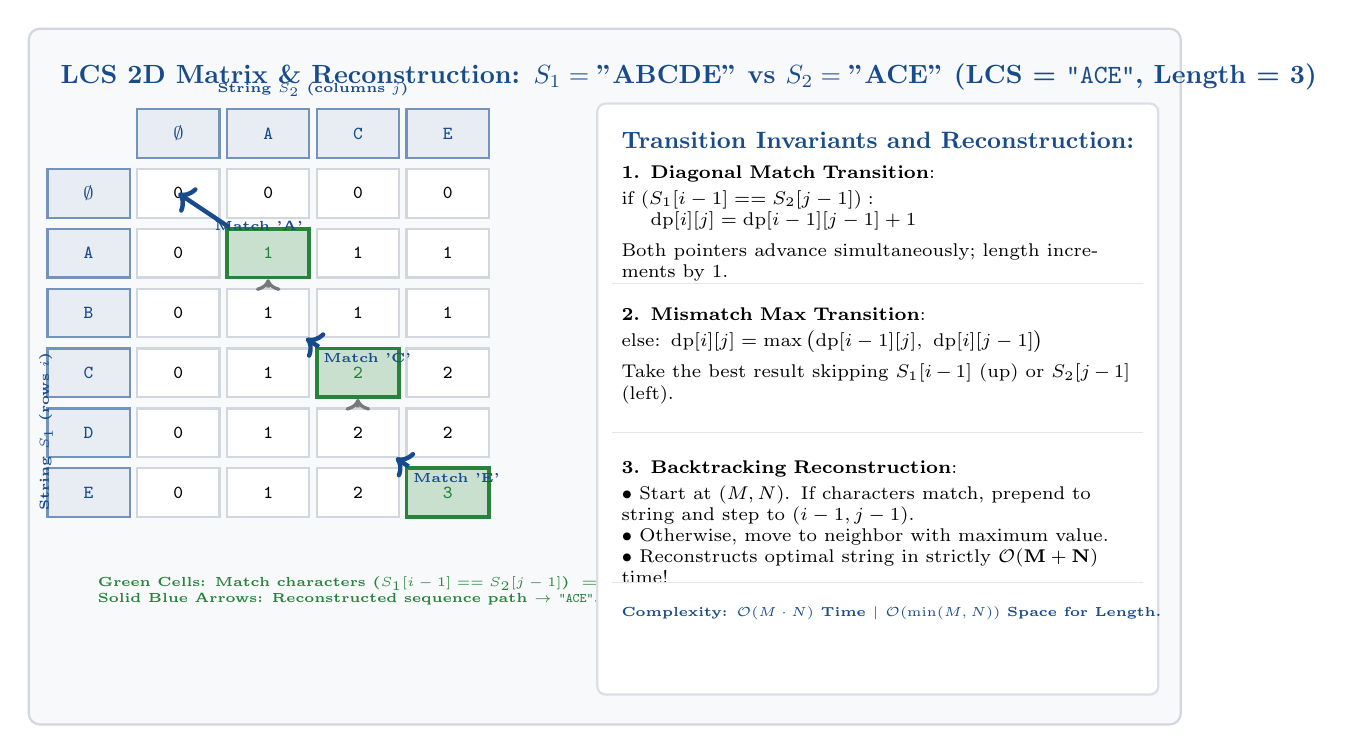
\begin{tikzpicture}[
    scale=0.95, every node/.style={transform shape},
    cell/.style={draw=codeframe, fill=white, thick, minimum width=1.1cm, minimum height=0.65cm, font=\scriptsize\ttfamily, align=center},
    matchCell/.style={draw=codegreen, fill=codegreen!25, line width=1.3pt, minimum width=1.1cm, minimum height=0.65cm, font=\scriptsize\bfseries\ttfamily, text=codegreen, align=center},
    headCell/.style={draw=primaryblue!60, fill=primaryblue!10, thick, minimum width=1.1cm, minimum height=0.65cm, font=\scriptsize\bfseries\ttfamily, text=primaryblue, align=center},
    card/.style={draw=codeframe, fill=codebg, rounded corners=4pt, thick}
]
    % Container Frame
    \draw[card] (0.0, -4.5) rectangle (15.4, 4.8);
    \node[anchor=north west, font=\bfseries\normalsize, text=primaryblue] at (0.3, 4.45) {LCS 2D Matrix \& Reconstruction: $S_1 = \text{"ABCDE"}$ vs $S_2 = \text{"ACE"}$ (LCS = \texttt{"ACE"}, Length = 3)};

    % --- Left Panel: 2D Matrix (x: 0.5 to 7.8, y: 3.6 to -4.0) ---
    % Column Headers (S2: \emptyset, A, C, E at x = 2.0, 3.2, 4.4, 5.6)
    \node[headCell] at (2.0, 3.4) {$\emptyset$};
    \node[headCell] at (3.2, 3.4) {A};
    \node[headCell] at (4.4, 3.4) {C};
    \node[headCell] at (5.6, 3.4) {E};
    \node[above=2pt, font=\tiny\bfseries, text=primaryblue] at (3.8, 3.7) {String $S_2$ (columns $j$)};

    % Row Headers (S1: \emptyset, A, B, C, D, E at y = 2.6 down to -1.4)
    \node[headCell] at (0.8, 2.6) {$\emptyset$};
    \node[headCell] at (0.8, 1.8) {A};
    \node[headCell] at (0.8, 1.0) {B};
    \node[headCell] at (0.8, 0.2) {C};
    \node[headCell] at (0.8, -0.6) {D};
    \node[headCell] at (0.8, -1.4) {E};
    \node[left=2pt, font=\tiny\bfseries, text=primaryblue, rotate=90] at (0.3, 0.6) {String $S_1$ (rows $i$)};

    % Matrix cells (row 0 to 5)
    % Row 0 (\emptyset): 0, 0, 0, 0
    \foreach \j/\val in {0/0, 1/0, 2/0, 3/0} { \node[cell] at (2.0 + \j*1.2, 2.6) {\val}; }
    % Row 1 (A): 0, 1*, 1, 1
    \node[cell] at (2.0, 1.8) {0};
    \node[matchCell] (C11) at (3.2, 1.8) {1};
    \node[cell] at (4.4, 1.8) {1};
    \node[cell] at (5.6, 1.8) {1};

    % Row 2 (B): 0, 1, 1, 1
    \node[cell] at (2.0, 1.0) {0};
    \node[cell] (C21) at (3.2, 1.0) {1};
    \node[cell] at (4.4, 1.0) {1};
    \node[cell] at (5.6, 1.0) {1};

    % Row 3 (C): 0, 1, 2*, 2
    \node[cell] at (2.0, 0.2) {0};
    \node[cell] at (3.2, 0.2) {1};
    \node[matchCell] (C32) at (4.4, 0.2) {2};
    \node[cell] at (5.6, 0.2) {2};

    % Row 4 (D): 0, 1, 2, 2
    \node[cell] at (2.0, -0.6) {0};
    \node[cell] at (3.2, -0.6) {1};
    \node[cell] (C42) at (4.4, -0.6) {2};
    \node[cell] at (5.6, -0.6) {2};

    % Row 5 (E): 0, 1, 2, 3*
    \node[cell] at (2.0, -1.4) {0};
    \node[cell] at (3.2, -1.4) {1};
    \node[cell] at (4.4, -1.4) {2};
    \node[matchCell] (C53) at (5.6, -1.4) {3};

    % Reconstruction Arrows (backwards from 5,3 -> 4,2 -> 3,2 -> 2,1 -> 1,1 -> 0,0)
    \draw[->, line width=1.6pt, primaryblue] (C53) -- (C42) node[midway, below right, font=\tiny\bfseries] {Match 'E'};
    \draw[->, line width=1.2pt, codegray, dashed] (C42) -- (C32);
    \draw[->, line width=1.6pt, primaryblue] (C32) -- (C21) node[midway, below right, font=\tiny\bfseries] {Match 'C'};
    \draw[->, line width=1.2pt, codegray, dashed] (C21) -- (C11);
    \draw[->, line width=1.6pt, primaryblue] (C11) -- (2.0, 2.6) node[midway, below right, font=\tiny\bfseries] {Match 'A'};

    \node[anchor=north west, font=\tiny\bfseries, text=codegreen, align=left] at (0.8, -2.4) {
        Green Cells: Match characters ($S_1[i-1] == S_2[j-1]$) $\implies \text{dp}[i-1][j-1] + 1$.\\
        Solid Blue Arrows: Reconstructed sequence path $\to$ \texttt{"ACE"}.
    };

    % --- Right Panel: Rules & Complexity (x: 7.6 to 15.1) ---
    \draw[draw=codeframe!80, fill=white, rounded corners=3pt, thick] (7.6, -4.1) rectangle (15.1, 3.8);
    \node[anchor=north west, font=\small\bfseries, text=primaryblue] at (7.8, 3.55) {Transition Invariants and Reconstruction:};

    \node[anchor=north west, font=\scriptsize, align=left, text width=6.8cm] at (7.8, 3.1) {
        \textbf{1. Diagonal Match Transition}:\\[2pt]
        $\text{if } (S_1[i-1] == S_2[j-1]):$\\
        \phantom{xx} $\text{dp}[i][j] = \text{dp}[i-1][j-1] + 1$\\[4pt]
        Both pointers advance simultaneously; length increments by $1$.
    };

    \draw[draw=codeframe!60] (7.8, 1.4) -- (14.9, 1.4);

    \node[anchor=north west, font=\scriptsize, align=left, text width=6.8cm] at (7.8, 1.2) {
        \textbf{2. Mismatch Max Transition}:\\[2pt]
        $\text{else: } \text{dp}[i][j] = \max\big( \text{dp}[i-1][j], \ \text{dp}[i][j-1] \big)$\\[4pt]
        Take the best result skipping $S_1[i-1]$ (up) or $S_2[j-1]$ (left).
    };

    \draw[draw=codeframe!60] (7.8, -0.6) -- (14.9, -0.6);

    \node[anchor=north west, font=\scriptsize, align=left, text width=6.8cm] at (7.8, -0.85) {
        \textbf{3. Backtracking Reconstruction}:\\[2pt]
        $\bullet$ Start at $(M, N)$. If characters match, prepend to string and step to $(i-1, j-1)$.\\
        $\bullet$ Otherwise, move to neighbor with maximum value.\\
        $\bullet$ Reconstructs optimal string in strictly $\mathbf{\mathcal{O}(M + N)}$ time!
    };

    \draw[draw=codeframe!60] (7.8, -2.6) -- (14.9, -2.6);

    \node[anchor=north west, font=\tiny\bfseries, text=primaryblue] at (7.8, -2.8) {
        Complexity: $\mathcal{O}(M \cdot N)$ Time $\mid$ $\mathcal{O}(\min(M,N))$ Space for Length.
    };
\end{tikzpicture}}
\caption{Longest Common Subsequence (LCS) 2D state matrix and reconstruction path. Diagonal steps (green) represent matched character contributions, while backwards tracing from $(M, N)$ recovers the optimal common subsequence \texttt{"ACE"} in $O(M + N)$ time.}
\end{figure}

\newpage
\newpage
\newpage

\subsection[Diagram 35: DAG Topological Sorting and Kahn's Algorithm]{Diagram 35: Directed Acyclic Graph (DAG) Topological Sorting \& Kahn's In-Degree Algorithm}

\breadcrumb{07.graph_algorithms.tex}{Section 2.4: Topological Sorting and Cycle Detection}{Visualizes in-degree initialization, frontier queue processing, dynamic edge elimination, and final linear order generation.}

\diagramaudit{Agent (Antigravity)}{2026-10-12}{Constructed full-width 2-panel architecture: left panel shows DAG structure with dynamic in-degree reduction and queue trace; right panel summarizes Kahn's invariant, cycle detection condition, and O(V + E) complexity guarantees.}

\begin{figure}[htbp]
\centering
\noindent\resizebox{\textwidth}{!}{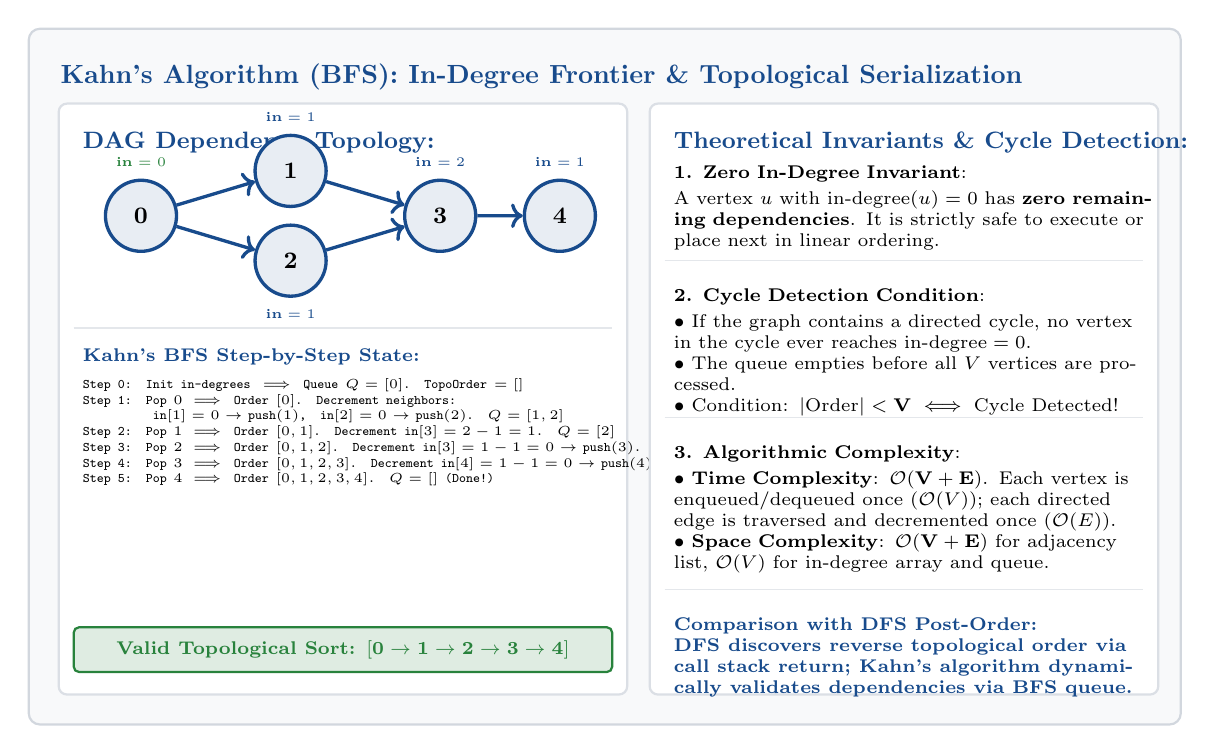
\begin{tikzpicture}[
    scale=0.95, every node/.style={transform shape},
    vNode/.style={circle, draw=primaryblue, fill=primaryblue!10, very thick, minimum size=0.95cm, font=\small\bfseries, align=center},
    activeNode/.style={circle, draw=codegreen, fill=codegreen!20, line width=1.5pt, minimum size=0.95cm, font=\small\bfseries, text=codegreen, align=center},
    doneNode/.style={circle, draw=codegray, fill=codeframe!40, thick, minimum size=0.95cm, font=\small\bfseries, text=codegray, align=center},
    qCell/.style={draw=codeframe, fill=white, thick, minimum width=0.8cm, minimum height=0.55cm, font=\scriptsize\ttfamily, align=center},
    card/.style={draw=codeframe, fill=codebg, rounded corners=4pt, thick}
]
    % Container Frame
    \draw[card] (0.0, -4.5) rectangle (15.4, 4.8);
    \node[anchor=north west, font=\bfseries\normalsize, text=primaryblue] at (0.3, 4.45) {Kahn's Algorithm (BFS): In-Degree Frontier \& Topological Serialization};

    % --- Left Panel: DAG & Queue Steps (x: 0.4 to 8.0) ---
    \draw[draw=codeframe!80, fill=white, rounded corners=3pt, thick] (0.4, -4.1) rectangle (8.0, 3.8);
    \node[anchor=north west, font=\small\bfseries, text=primaryblue] at (0.6, 3.55) {DAG Dependency Topology:};

    % Vertices layout
    \node[vNode] (N0) at (1.5, 2.3) {0};
    \node[vNode] (N1) at (3.5, 2.9) {1};
    \node[vNode] (N2) at (3.5, 1.7) {2};
    \node[vNode] (N3) at (5.5, 2.3) {3};
    \node[vNode] (N4) at (7.1, 2.3) {4};

    % Initial in-degree badges
    \node[above=1pt of N0, font=\tiny\bfseries, text=codegreen] {$\text{in}=0$};
    \node[above=1pt of N1, font=\tiny\bfseries, text=primaryblue] {$\text{in}=1$};
    \node[below=1pt of N2, font=\tiny\bfseries, text=primaryblue] {$\text{in}=1$};
    \node[above=1pt of N3, font=\tiny\bfseries, text=primaryblue] {$\text{in}=2$};
    \node[above=1pt of N4, font=\tiny\bfseries, text=primaryblue] {$\text{in}=1$};

    % Directed edges
    \draw[->, line width=1.2pt, primaryblue] (N0) -- (N1);
    \draw[->, line width=1.2pt, primaryblue] (N0) -- (N2);
    \draw[->, line width=1.2pt, primaryblue] (N1) -- (N3);
    \draw[->, line width=1.2pt, primaryblue] (N2) -- (N3);
    \draw[->, line width=1.2pt, primaryblue] (N3) -- (N4);

    % Execution Trace Table
    \draw[draw=codeframe!60] (0.6, 0.8) -- (7.8, 0.8);
    \node[anchor=north west, font=\scriptsize\bfseries, text=primaryblue] at (0.6, 0.65) {Kahn's BFS Step-by-Step State:};

    \node[anchor=north west, font=\tiny\ttfamily, align=left] at (0.6, 0.25) {
        \textbf{Step 0}: Init in-degrees $\implies$ Queue $Q = [0]$. TopoOrder $= []$\\
        \textbf{Step 1}: Pop $0 \implies$ Order $[0]$. Decrement neighbors:\\
        \phantom{Step 1: } $\text{in}[1] = 0 \to \text{push}(1)$, \ $\text{in}[2] = 0 \to \text{push}(2)$. $Q = [1, 2]$\\
        \textbf{Step 2}: Pop $1 \implies$ Order $[0, 1]$. Decrement $\text{in}[3] = 2-1 = 1$. $Q = [2]$\\
        \textbf{Step 3}: Pop $2 \implies$ Order $[0, 1, 2]$. Decrement $\text{in}[3] = 1-1 = 0 \to \text{push}(3)$. $Q = [3]$\\
        \textbf{Step 4}: Pop $3 \implies$ Order $[0, 1, 2, 3]$. Decrement $\text{in}[4] = 1-1 = 0 \to \text{push}(4)$. $Q = [4]$\\
        \textbf{Step 5}: Pop $4 \implies$ Order $[0, 1, 2, 3, 4]$. $Q = []$ (Done!)
    };

    % Result Order Badge
    \draw[fill=codegreen!15, draw=codegreen, rounded corners=2pt, thick] (0.6, -3.8) rectangle (7.8, -3.2);
    \node[font=\scriptsize\bfseries, text=codegreen] at (4.2, -3.5) {Valid Topological Sort: $\mathbf{[0 \to 1 \to 2 \to 3 \to 4]}$};

    % --- Right Panel: Invariants & Analysis (x: 8.3 to 15.1) ---
    \draw[draw=codeframe!80, fill=white, rounded corners=3pt, thick] (8.3, -4.1) rectangle (15.1, 3.8);
    \node[anchor=north west, font=\small\bfseries, text=primaryblue] at (8.5, 3.55) {Theoretical Invariants \& Cycle Detection:};

    \node[anchor=north west, font=\scriptsize, align=left, text width=6.4cm] at (8.5, 3.1) {
        \textbf{1. Zero In-Degree Invariant}:\\[2pt]
        A vertex $u$ with $\text{in-degree}(u) = 0$ has \textbf{zero remaining dependencies}. It is strictly safe to execute or place next in linear ordering.
    };

    \draw[draw=codeframe!60] (8.5, 1.7) -- (14.9, 1.7);

    \node[anchor=north west, font=\scriptsize, align=left, text width=6.4cm] at (8.5, 1.45) {
        \textbf{2. Cycle Detection Condition}:\\[2pt]
        $\bullet$ If the graph contains a directed cycle, no vertex in the cycle ever reaches $\text{in-degree} = 0$.\\
        $\bullet$ The queue empties before all $V$ vertices are processed.\\
        $\bullet$ Condition: $\mathbf{|\text{Order}| < V \iff \text{Cycle Detected!}}$
    };

    \draw[draw=codeframe!60] (8.5, -0.4) -- (14.9, -0.4);

    \node[anchor=north west, font=\scriptsize, align=left, text width=6.4cm] at (8.5, -0.65) {
        \textbf{3. Algorithmic Complexity}:\\[2pt]
        $\bullet$ \textbf{Time Complexity}: $\mathbf{\mathcal{O}(V + E)}$. Each vertex is enqueued/dequeued once ($\mathcal{O}(V)$); each directed edge is traversed and decremented once ($\mathcal{O}(E)$).\\
        $\bullet$ \textbf{Space Complexity}: $\mathbf{\mathcal{O}(V + E)}$ for adjacency list, $\mathcal{O}(V)$ for in-degree array and queue.
    };

    \draw[draw=codeframe!60] (8.5, -2.7) -- (14.9, -2.7);

    \node[anchor=north west, font=\scriptsize\bfseries, text=primaryblue, align=left, text width=6.4cm] at (8.5, -2.95) {
        Comparison with DFS Post-Order:\\
        DFS discovers reverse topological order via call stack return; Kahn's algorithm dynamically validates dependencies via BFS queue.
    };
\end{tikzpicture}}
\caption{Kahn's in-degree queue algorithm for topological sorting of Directed Acyclic Graphs (DAGs). Dynamically decrementing edge dependencies guarantees correct task serialization and identifies cycles when $|\text{Order}| < V$.}
\end{figure}

\newpage
\newpage
\newpage

\subsection[Diagram 36: Bipartite 2-Coloring and Odd Cycle Contradiction]{Diagram 36: Bipartite Graph Checking (2-Coloring) \& Odd Cycle Contradiction Detection}

\breadcrumb{07.graph_algorithms.tex}{Section 2.7: Bipartite Graphs and 2-Coloring}{Visualizes vertex partition into two independent sets $U$ and $V$, and proves why an odd-length cycle creates an unavoidable monochromatic edge conflict.}

\diagramaudit{Agent (Antigravity)}{2026-10-12}{Constructed full-width 2-panel architecture: left panel shows valid bipartite 2-coloring across partition sets U and V; right panel illustrates odd-cycle C3/C5 coloring deadlock and states the fundamental bipartition theorem.}

\begin{figure}[htbp]
\centering
\noindent\resizebox{\textwidth}{!}{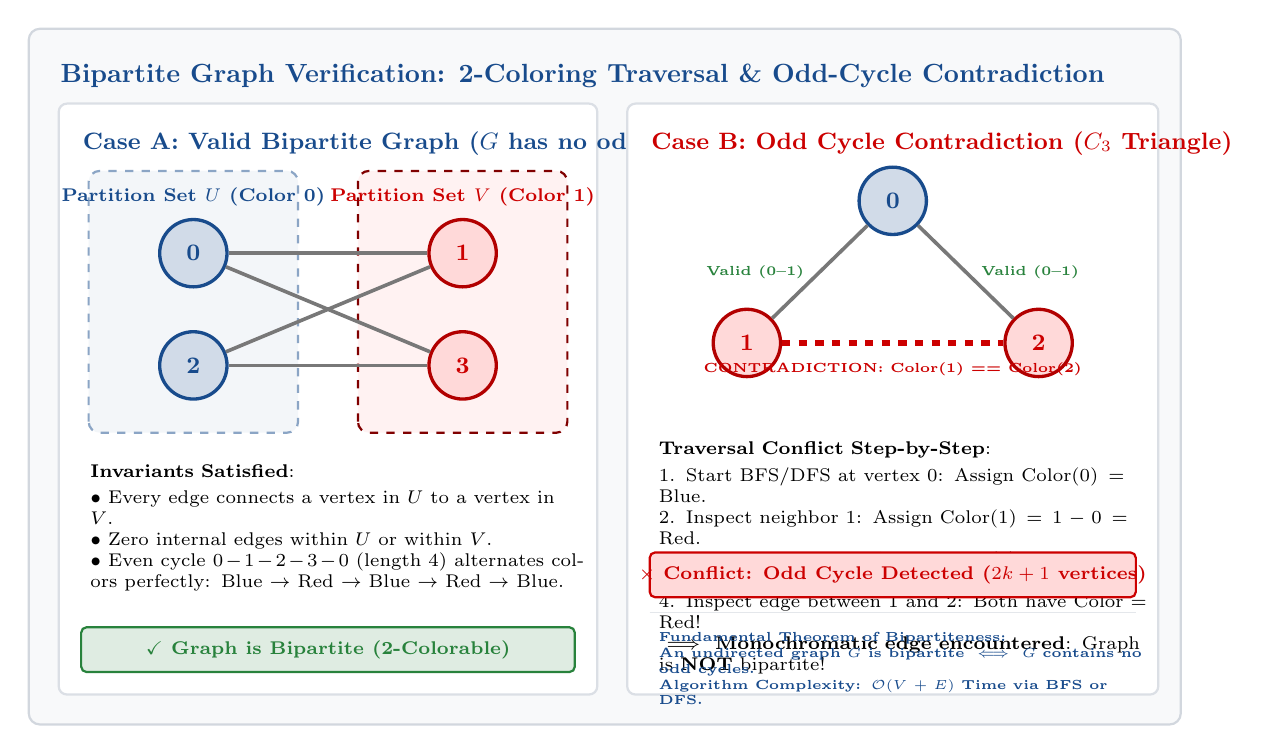
\begin{tikzpicture}[
    scale=0.95, every node/.style={transform shape},
    nodeBlue/.style={circle, draw=primaryblue, fill=primaryblue!20, very thick, minimum size=0.9cm, font=\small\bfseries, text=primaryblue, align=center},
    nodeRed/.style={circle, draw=red!70!black, fill=red!15, very thick, minimum size=0.9cm, font=\small\bfseries, text=red!80!black, align=center},
    card/.style={draw=codeframe, fill=codebg, rounded corners=4pt, thick}
]
    % Container Frame
    \draw[card] (0.0, -4.5) rectangle (15.4, 4.8);
    \node[anchor=north west, font=\bfseries\normalsize, text=primaryblue] at (0.3, 4.45) {Bipartite Graph Verification: 2-Coloring Traversal \& Odd-Cycle Contradiction};

    % --- Left Panel: Valid Bipartite Partition (x: 0.4 to 7.6) ---
    \draw[draw=codeframe!80, fill=white, rounded corners=3pt, thick] (0.4, -4.1) rectangle (7.6, 3.8);
    \node[anchor=north west, font=\small\bfseries, text=primaryblue] at (0.6, 3.55) {Case A: Valid Bipartite Graph ($G$ has no odd cycles)};

    % Partition Sets (U on left, V on right)
    \draw[draw=primaryblue!50, fill=primaryblue!5, dashed, rounded corners=4pt, thick] (0.8, -0.6) rectangle (3.6, 2.9);
    \node[anchor=north, font=\scriptsize\bfseries, text=primaryblue] at (2.2, 2.8) {Partition Set $U$ (Color 0)};

    \draw[draw=red!50!black, fill=red!5, dashed, rounded corners=4pt, thick] (4.4, -0.6) rectangle (7.2, 2.9);
    \node[anchor=north, font=\scriptsize\bfseries, text=red!80!black] at (5.8, 2.8) {Partition Set $V$ (Color 1)};

    % Nodes in Set U
    \node[nodeBlue] (U1) at (2.2, 1.8) {0};
    \node[nodeBlue] (U2) at (2.2, 0.3) {2};

    % Nodes in Set V
    \node[nodeRed] (V1) at (5.8, 1.8) {1};
    \node[nodeRed] (V2) at (5.8, 0.3) {3};

    % Crossing Edges (All valid!)
    \draw[line width=1.3pt, codegray] (U1) -- (V1);
    \draw[line width=1.3pt, codegray] (U1) -- (V2);
    \draw[line width=1.3pt, codegray] (U2) -- (V1);
    \draw[line width=1.3pt, codegray] (U2) -- (V2);

    \node[anchor=north west, font=\scriptsize, align=left, text width=6.6cm] at (0.7, -0.9) {
        \textbf{Invariants Satisfied}:\\[2pt]
        $\bullet$ Every edge connects a vertex in $U$ to a vertex in $V$.\\
        $\bullet$ Zero internal edges within $U$ or within $V$.\\
        $\bullet$ Even cycle $0 - 1 - 2 - 3 - 0$ (length 4) alternates colors perfectly: Blue $\to$ Red $\to$ Blue $\to$ Red $\to$ Blue.
    };

    \draw[fill=codegreen!15, draw=codegreen, rounded corners=2pt, thick] (0.7, -3.8) rectangle (7.3, -3.2);
    \node[font=\scriptsize\bfseries, text=codegreen] at (4.0, -3.5) {$\checkmark$ Graph is Bipartite (2-Colorable)};

    % --- Right Panel: Odd Cycle Contradiction (x: 8.0 to 15.1) ---
    \draw[draw=codeframe!80, fill=white, rounded corners=3pt, thick] (8.0, -4.1) rectangle (15.1, 3.8);
    \node[anchor=north west, font=\small\bfseries, text=red!80!black] at (8.2, 3.55) {Case B: Odd Cycle Contradiction ($C_3$ Triangle)};

    % Triangle Nodes
    \node[nodeBlue] (T0) at (11.55, 2.5) {0};
    \node[nodeRed]  (T1) at (9.6, 0.6) {1};
    \node[nodeRed]  (T2) at (13.5, 0.6) {2};

    % Edges
    \draw[line width=1.3pt, codegray] (T0) -- (T1) node[midway, left=2pt, font=\tiny\bfseries, text=codegreen] {Valid (0--1)};
    \draw[line width=1.3pt, codegray] (T0) -- (T2) node[midway, right=2pt, font=\tiny\bfseries, text=codegreen] {Valid (0--1)};
    \draw[line width=2.0pt, red!80!black, dashed] (T1) -- (T2) node[midway, below=3pt, font=\tiny\bfseries, text=red!80!black] {CONTRADICTION: Color(1) == Color(2)};

    \node[anchor=north west, font=\scriptsize, align=left, text width=6.6cm] at (8.3, -0.6) {
        \textbf{Traversal Conflict Step-by-Step}:\\[2pt]
        1. Start BFS/DFS at vertex $0$: Assign $\text{Color}(0) = \text{Blue}$.\\
        2. Inspect neighbor $1$: Assign $\text{Color}(1) = 1 - 0 = \text{Red}$.\\
        3. Inspect neighbor $2$: Assign $\text{Color}(2) = 1 - 0 = \text{Red}$.\\
        4. Inspect edge between $1$ and $2$: Both have $\text{Color} = \text{Red}$!\\
        $\implies$ \textbf{Monochromatic edge encountered}: Graph is \textbf{NOT} bipartite!
    };

    \draw[fill=red!15, draw=red!80!black, rounded corners=2pt, thick] (8.3, -2.8) rectangle (14.8, -2.2);
    \node[font=\scriptsize\bfseries, text=red!80!black] at (11.55, -2.5) {$\times$ Conflict: Odd Cycle Detected ($2k+1$ vertices)};

    \draw[draw=codeframe!60] (8.3, -3.0) -- (14.8, -3.0);
    \node[anchor=north west, font=\tiny\bfseries, text=primaryblue, align=left, text width=6.5cm] at (8.3, -3.15) {
        \textbf{Fundamental Theorem of Bipartiteness}:\\
        An undirected graph $G$ is bipartite $\iff$ $G$ contains no odd cycles.\\
        Algorithm Complexity: $\mathcal{O}(V + E)$ Time via BFS or DFS.
    };
\end{tikzpicture}}
\caption{Bipartite graph verification and 2-coloring. Left: Valid bipartition into sets $U$ and $V$ with alternating edge endpoints. Right: Odd cycle contradiction where two adjacent vertices are forced to share the same color, violating the bipartition invariant.}
\end{figure}

\newpage
\newpage
\newpage

\subsection[Diagram 37: Search in Rotated Sorted Array]{Diagram 37: Search in Rotated Sorted Array: Discontinuity Pivot \& Monotonic Halves}

\breadcrumb{08.binary_search.tex}{Section 2.5: Searching in Rotated Sorted Arrays}{Visualizes two monotonic sorted segments separated by a rotation pivot drop, and the deterministic binary search half-selection rules.}

\diagramaudit{Agent (Antigravity)}{2026-10-12}{Constructed full-width 2-panel architecture: left panel plots piecewise monotonic elevation profile and array cell indices; right panel formalizes the binary search branch invariants and guarantees O(log N) query time.}

\begin{figure}[htbp]
\centering
\noindent\resizebox{\textwidth}{!}{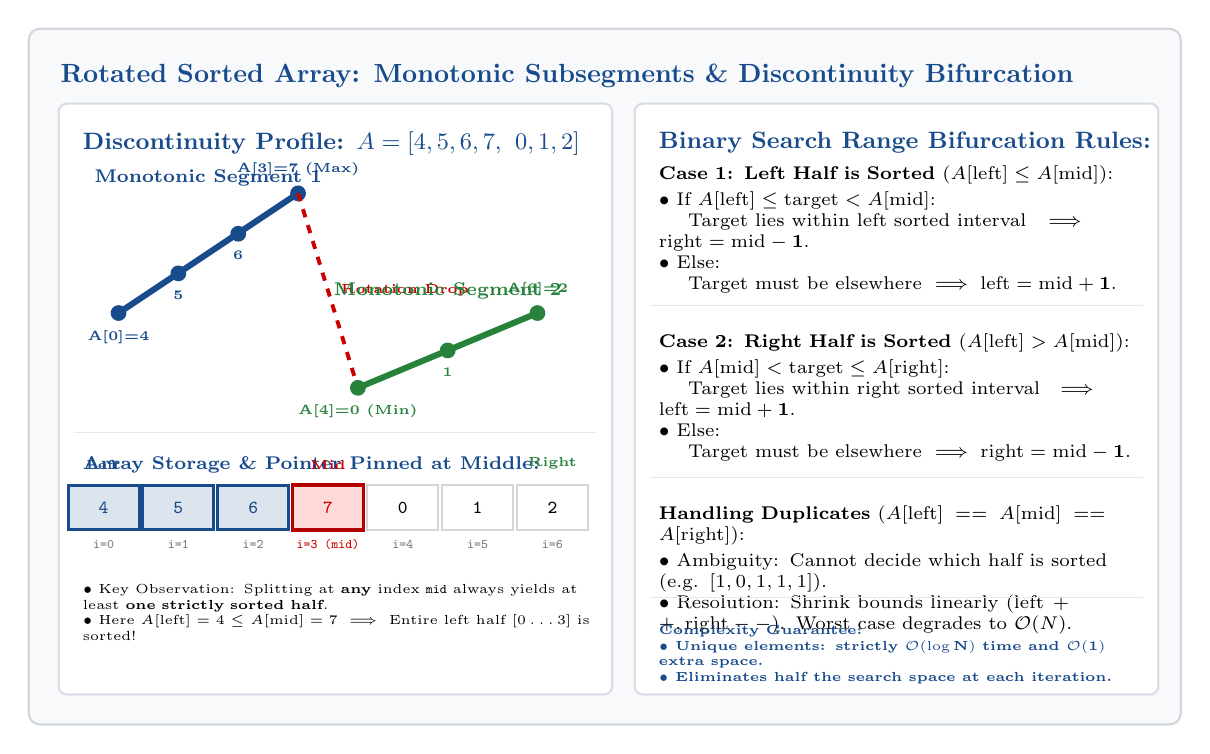
\begin{tikzpicture}[
    scale=0.95, every node/.style={transform shape},
    cell/.style={draw=codeframe, fill=white, thick, minimum width=0.95cm, minimum height=0.6cm, font=\scriptsize\ttfamily, align=center},
    pivotCell/.style={draw=red!70!black, fill=red!15, line width=1.2pt, minimum width=0.95cm, minimum height=0.6cm, font=\scriptsize\bfseries\ttfamily, text=red!80!black, align=center},
    sortedCell/.style={draw=primaryblue, fill=primaryblue!15, line width=1.1pt, minimum width=0.95cm, minimum height=0.6cm, font=\scriptsize\bfseries\ttfamily, text=primaryblue, align=center},
    card/.style={draw=codeframe, fill=codebg, rounded corners=4pt, thick}
]
    % Container Frame
    \draw[card] (0.0, -4.5) rectangle (15.4, 4.8);
    \node[anchor=north west, font=\bfseries\normalsize, text=primaryblue] at (0.3, 4.45) {Rotated Sorted Array: Monotonic Subsegments \& Discontinuity Bifurcation};

    % --- Left Panel: Elevation Profile & Array Grid (x: 0.4 to 7.8) ---
    \draw[draw=codeframe!80, fill=white, rounded corners=3pt, thick] (0.4, -4.1) rectangle (7.8, 3.8);
    \node[anchor=north west, font=\small\bfseries, text=primaryblue] at (0.6, 3.55) {Discontinuity Profile: $A = [4, 5, 6, 7, \ 0, 1, 2]$};

    % Plotting the two ramps
    % Ramp 1: (1.2, 1.0) to (3.6, 2.5) for [4, 5, 6, 7]
    \draw[line width=2.2pt, primaryblue] (1.2, 1.0) -- (3.6, 2.6);
    \fill[primaryblue] (1.2, 1.0) circle (3pt) node[below=3pt, font=\tiny\bfseries] {A[0]=4};
    \fill[primaryblue] (2.0, 1.53) circle (3pt) node[below=3pt, font=\tiny\bfseries] {5};
    \fill[primaryblue] (2.8, 2.06) circle (3pt) node[below=3pt, font=\tiny\bfseries] {6};
    \fill[primaryblue] (3.6, 2.6) circle (3pt) node[above=3pt, font=\tiny\bfseries] {A[3]=7 (Max)};

    % Discontinuity drop line
    \draw[dashed, line width=1.4pt, red!80!black] (3.6, 2.6) -- (4.4, 0.0) node[midway, right=1pt, font=\tiny\bfseries, text=red!80!black] {Rotation Drop};

    % Ramp 2: (4.4, 0.0) to (6.8, 1.0) for [0, 1, 2]
    \draw[line width=2.2pt, codegreen] (4.4, 0.0) -- (6.8, 1.0);
    \fill[codegreen] (4.4, 0.0) circle (3pt) node[below=3pt, font=\tiny\bfseries] {A[4]=0 (Min)};
    \fill[codegreen] (5.6, 0.5) circle (3pt) node[below=3pt, font=\tiny\bfseries] {1};
    \fill[codegreen] (6.8, 1.0) circle (3pt) node[above=3pt, font=\tiny\bfseries] {A[6]=2};

    % Labels for Ramps
    \node[font=\scriptsize\bfseries, text=primaryblue] at (2.4, 2.8) {Monotonic Segment 1};
    \node[font=\scriptsize\bfseries, text=codegreen] at (5.6, 1.3) {Monotonic Segment 2};

    % Array visual cells below plot
    \draw[draw=codeframe!60] (0.6, -0.6) -- (7.6, -0.6);
    \node[anchor=north west, font=\scriptsize\bfseries, text=primaryblue] at (0.6, -0.8) {Array Storage \& Pointer Pinned at Middle:};

    % Cells for indices 0 to 6 at y = -1.6
    \node[sortedCell] at (1.0, -1.6) {4};
    \node[sortedCell] at (2.0, -1.6) {5};
    \node[sortedCell] at (3.0, -1.6) {6};
    \node[pivotCell]  at (4.0, -1.6) {7};
    \node[cell]       at (5.0, -1.6) {0};
    \node[cell]       at (6.0, -1.6) {1};
    \node[cell]       at (7.0, -1.6) {2};

    % Indices
    \node[font=\tiny\ttfamily, text=codegray] at (1.0, -2.1) {i=0};
    \node[font=\tiny\ttfamily, text=codegray] at (2.0, -2.1) {i=1};
    \node[font=\tiny\ttfamily, text=codegray] at (3.0, -2.1) {i=2};
    \node[font=\tiny\ttfamily, text=red!80!black] at (4.0, -2.1) {i=3 (mid)};
    \node[font=\tiny\ttfamily, text=codegray] at (5.0, -2.1) {i=4};
    \node[font=\tiny\ttfamily, text=codegray] at (6.0, -2.1) {i=5};
    \node[font=\tiny\ttfamily, text=codegray] at (7.0, -2.1) {i=6};

    % Pointer indicators
    \node[above=1pt, font=\tiny\bfseries, text=primaryblue] at (1.0, -1.25) {Left};
    \node[above=1pt, font=\tiny\bfseries, text=red!80!black] at (4.0, -1.25) {Mid};
    \node[above=1pt, font=\tiny\bfseries, text=codegreen] at (7.0, -1.25) {Right};

    \node[anchor=north west, font=\tiny, align=left, text width=6.8cm] at (0.6, -2.5) {
        $\bullet$ Key Observation: Splitting at \textbf{any} index \texttt{mid} always yields at least \textbf{one strictly sorted half}.\\
        $\bullet$ Here $A[\text{left}] = 4 \le A[\text{mid}] = 7 \implies$ Entire left half $[0 \dots 3]$ is sorted!
    };

    % --- Right Panel: Binary Search Invariants (x: 8.1 to 15.1) ---
    \draw[draw=codeframe!80, fill=white, rounded corners=3pt, thick] (8.1, -4.1) rectangle (15.1, 3.8);
    \node[anchor=north west, font=\small\bfseries, text=primaryblue] at (8.3, 3.55) {Binary Search Range Bifurcation Rules:};

    \node[anchor=north west, font=\scriptsize, align=left, text width=6.5cm] at (8.3, 3.1) {
        \textbf{Case 1: Left Half is Sorted} ($A[\text{left}] \le A[\text{mid}]$):\\[2pt]
        $\bullet$ If $A[\text{left}] \le \text{target} < A[\text{mid}]$:\\
        \phantom{xx} Target lies within left sorted interval $\implies \mathbf{\text{right} = \text{mid} - 1}$.\\
        $\bullet$ Else:\\
        \phantom{xx} Target must be elsewhere $\implies \mathbf{\text{left} = \text{mid} + 1}$.
    };

    \draw[draw=codeframe!60] (8.3, 1.1) -- (14.9, 1.1);

    \node[anchor=north west, font=\scriptsize, align=left, text width=6.5cm] at (8.3, 0.85) {
        \textbf{Case 2: Right Half is Sorted} ($A[\text{left}] > A[\text{mid}]$):\\[2pt]
        $\bullet$ If $A[\text{mid}] < \text{target} \le A[\text{right}]$:\\
        \phantom{xx} Target lies within right sorted interval $\implies \mathbf{\text{left} = \text{mid} + 1}$.\\
        $\bullet$ Else:\\
        \phantom{xx} Target must be elsewhere $\implies \mathbf{\text{right} = \text{mid} - 1}$.
    };

    \draw[draw=codeframe!60] (8.3, -1.2) -- (14.9, -1.2);

    \node[anchor=north west, font=\scriptsize, align=left, text width=6.5cm] at (8.3, -1.45) {
        \textbf{Handling Duplicates} ($A[\text{left}] == A[\text{mid}] == A[\text{right}]$):\\[2pt]
        $\bullet$ Ambiguity: Cannot decide which half is sorted (e.g. $[1, 0, 1, 1, 1]$).\\
        $\bullet$ Resolution: Shrink bounds linearly ($\text{left}++, \text{right}--$). Worst case degrades to $\mathcal{O}(N)$.
    };

    \draw[draw=codeframe!60] (8.3, -2.8) -- (14.9, -2.8);

    \node[anchor=north west, font=\tiny\bfseries, text=primaryblue, align=left, text width=6.5cm] at (8.3, -3.05) {
        Complexity Guarantee:\\
        $\bullet$ Unique elements: strictly $\mathbf{\mathcal{O}(\log N)}$ time and $\mathbf{\mathcal{O}(1)}$ extra space.\\
        $\bullet$ Eliminates half the search space at each iteration.
    };
\end{tikzpicture}}
\caption{Binary search in a rotated sorted array. Left: Elevation profile revealing two monotonic sorted ramps separated by a rotation pivot drop. Right: Branching rules identifying the sorted half to maintain $O(\log N)$ logarithmic convergence.}
\end{figure}

\newpage
\newpage
\newpage

\subsection[Diagram 38: Binary Exponentiation Repeated Squaring]{Diagram 38: Binary Exponentiation (Fast Power) Repeated Squaring \& Bit Decomposition}

\breadcrumb{02.number_theory.tex}{Section 2.1: Modular Arithmetic and Fast Exponentiation}{Visualizes logarithmic exponent decomposition ($n = \sum b_i 2^i$) and the state progression of base squaring and accumulator multiplication.}

\diagramaudit{Agent (Antigravity)}{2026-10-12}{Constructed full-width 2-panel architecture: left panel depicts bitwise decomposition of exponent 13 with base squaring and accumulator updates; right panel states recurrence relations, modular invariants, and O(log n) guarantees.}

\begin{figure}[htbp]
\centering
\noindent\resizebox{\textwidth}{!}{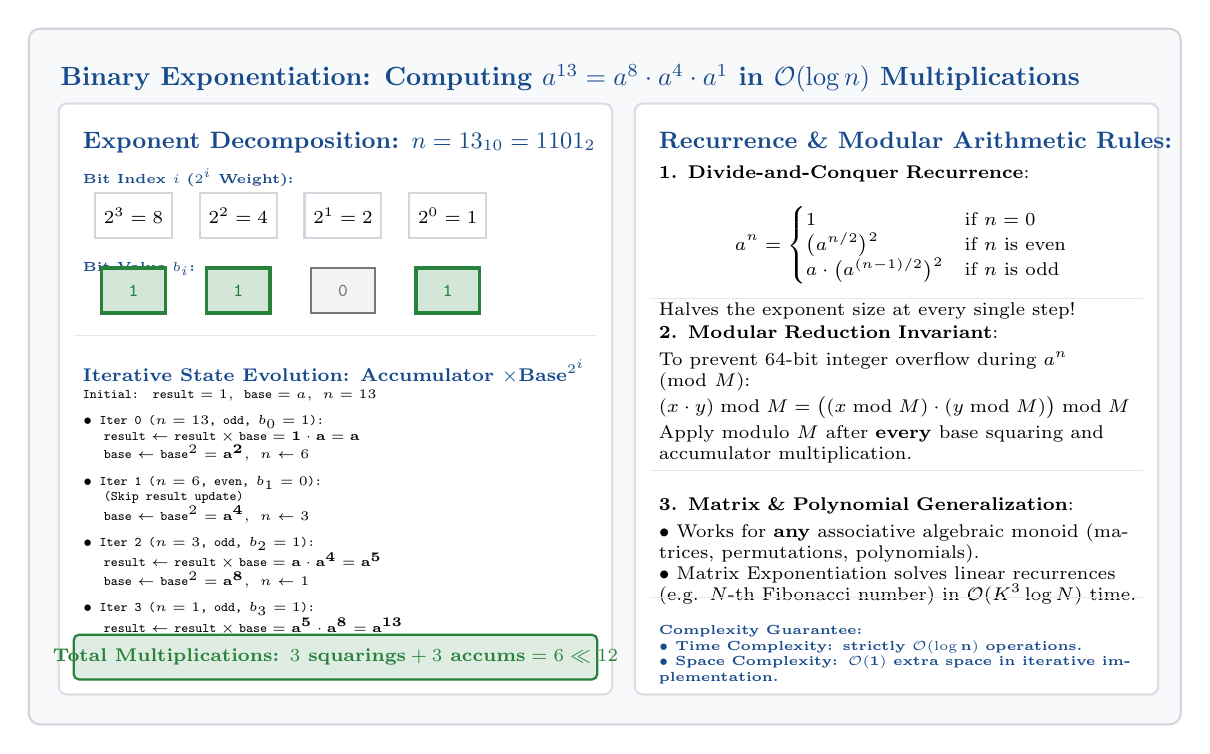
\begin{tikzpicture}[
    scale=0.95, every node/.style={transform shape},
    bitBox/.style={draw=codeframe, fill=white, thick, minimum width=0.85cm, minimum height=0.6cm, font=\scriptsize\ttfamily, align=center},
    bitActive/.style={draw=codegreen, fill=codegreen!20, line width=1.2pt, minimum width=0.85cm, minimum height=0.6cm, font=\scriptsize\bfseries\ttfamily, text=codegreen, align=center},
    bitInactive/.style={draw=codegray, fill=codeframe!30, thick, minimum width=0.85cm, minimum height=0.6cm, font=\scriptsize\ttfamily, text=codegray, align=center},
    card/.style={draw=codeframe, fill=codebg, rounded corners=4pt, thick}
]
    % Container Frame
    \draw[card] (0.0, -4.5) rectangle (15.4, 4.8);
    \node[anchor=north west, font=\bfseries\normalsize, text=primaryblue] at (0.3, 4.45) {Binary Exponentiation: Computing $a^{13} = a^8 \cdot a^4 \cdot a^1$ in $\mathcal{O}(\log n)$ Multiplications};

    % --- Left Panel: Bit Decomposition & Multiplier Flow (x: 0.4 to 7.8) ---
    \draw[draw=codeframe!80, fill=white, rounded corners=3pt, thick] (0.4, -4.1) rectangle (7.8, 3.8);
    \node[anchor=north west, font=\small\bfseries, text=primaryblue] at (0.6, 3.55) {Exponent Decomposition: $n = 13_{10} = 1101_2$};

    % Binary representation table
    \node[anchor=north west, font=\tiny\bfseries, text=primaryblue] at (0.6, 3.05) {Bit Index $i$ ($2^i$ Weight):};
    \node[bitBox] at (1.4, 2.3) {$2^3=8$};
    \node[bitBox] at (2.8, 2.3) {$2^2=4$};
    \node[bitBox] at (4.2, 2.3) {$2^1=2$};
    \node[bitBox] at (5.6, 2.3) {$2^0=1$};

    \node[anchor=north west, font=\tiny\bfseries, text=primaryblue] at (0.6, 1.8) {Bit Value $b_i$:};
    \node[bitActive]   at (1.4, 1.3) {\textbf{1}};
    \node[bitActive]   at (2.8, 1.3) {\textbf{1}};
    \node[bitInactive] at (4.2, 1.3) {0};
    \node[bitActive]   at (5.6, 1.3) {\textbf{1}};

    \draw[draw=codeframe!60] (0.6, 0.7) -- (7.6, 0.7);
    \node[anchor=north west, font=\scriptsize\bfseries, text=primaryblue] at (0.6, 0.5) {Iterative State Evolution: Accumulator $\times \text{Base}^{2^i}$};

    \node[anchor=north west, font=\tiny\ttfamily, align=left] at (0.6, 0.1) {
        \textbf{Initial}: $\text{result} = 1, \ \text{base} = a, \ n = 13$\\[4pt]
        $\bullet$ \textbf{Iter 0} ($n=13$, odd, $b_0=1$):\\
        \phantom{xx} $\text{result} \leftarrow \text{result} \times \text{base} = \mathbf{1 \cdot a = a}$\\
        \phantom{xx} $\text{base} \leftarrow \text{base}^2 = \mathbf{a^2}, \ n \leftarrow 6$\\[4pt]
        $\bullet$ \textbf{Iter 1} ($n=6$, even, $b_1=0$):\\
        \phantom{xx} (Skip result update)\\
        \phantom{xx} $\text{base} \leftarrow \text{base}^2 = \mathbf{a^4}, \ n \leftarrow 3$\\[4pt]
        $\bullet$ \textbf{Iter 2} ($n=3$, odd, $b_2=1$):\\
        \phantom{xx} $\text{result} \leftarrow \text{result} \times \text{base} = \mathbf{a \cdot a^4 = a^5}$\\
        \phantom{xx} $\text{base} \leftarrow \text{base}^2 = \mathbf{a^8}, \ n \leftarrow 1$\\[4pt]
        $\bullet$ \textbf{Iter 3} ($n=1$, odd, $b_3=1$):\\
        \phantom{xx} $\text{result} \leftarrow \text{result} \times \text{base} = \mathbf{a^5 \cdot a^8 = a^{13}}$\\
        \phantom{xx} $\text{base} \leftarrow \text{base}^2 = a^{16}, \ n \leftarrow 0 \implies \text{Done!}$
    };

    \draw[fill=codegreen!15, draw=codegreen, rounded corners=2pt, thick] (0.6, -3.9) rectangle (7.6, -3.3);
    \node[font=\scriptsize\bfseries, text=codegreen] at (4.1, -3.6) {Total Multiplications: $3 \text{ squarings} + 3 \text{ accums} = 6 \ll 12$};

    % --- Right Panel: Mathematical Rules (x: 8.1 to 15.1) ---
    \draw[draw=codeframe!80, fill=white, rounded corners=3pt, thick] (8.1, -4.1) rectangle (15.1, 3.8);
    \node[anchor=north west, font=\small\bfseries, text=primaryblue] at (8.3, 3.55) {Recurrence \& Modular Arithmetic Rules:};

    \node[anchor=north west, font=\scriptsize, align=left, text width=6.5cm] at (8.3, 3.1) {
        \textbf{1. Divide-and-Conquer Recurrence}:\\[2pt]
        $$a^n = \begin{cases}
        1 & \text{if } n = 0 \\
        \big(a^{n/2}\big)^2 & \text{if } n \text{ is even} \\
        a \cdot \big(a^{(n-1)/2}\big)^2 & \text{if } n \text{ is odd}
        \end{cases}$$
        Halves the exponent size at every single step!
    };

    \draw[draw=codeframe!60] (8.3, 1.2) -- (14.9, 1.2);

    \node[anchor=north west, font=\scriptsize, align=left, text width=6.5cm] at (8.3, 0.95) {
        \textbf{2. Modular Reduction Invariant}:\\[2pt]
        To prevent 64-bit integer overflow during $a^n \pmod M$:\\[2pt]
        $(x \cdot y) \bmod M = \big((x \bmod M) \cdot (y \bmod M)\big) \bmod M$\\[2pt]
        Apply modulo $M$ after \textbf{every} base squaring and accumulator multiplication.
    };

    \draw[draw=codeframe!60] (8.3, -1.1) -- (14.9, -1.1);

    \node[anchor=north west, font=\scriptsize, align=left, text width=6.5cm] at (8.3, -1.35) {
        \textbf{3. Matrix \& Polynomial Generalization}:\\[2pt]
        $\bullet$ Works for \textbf{any} associative algebraic monoid (matrices, permutations, polynomials).\\
        $\bullet$ Matrix Exponentiation solves linear recurrences (e.g. $N$-th Fibonacci number) in $\mathcal{O}(K^3 \log N)$ time.
    };

    \draw[draw=codeframe!60] (8.3, -2.8) -- (14.9, -2.8);

    \node[anchor=north west, font=\tiny\bfseries, text=primaryblue, align=left, text width=6.5cm] at (8.3, -3.05) {
        Complexity Guarantee:\\
        $\bullet$ Time Complexity: strictly $\mathbf{\mathcal{O}(\log n)}$ operations.\\
        $\bullet$ Space Complexity: $\mathbf{\mathcal{O}(1)}$ extra space in iterative implementation.
    };
\end{tikzpicture}}
\caption{Binary exponentiation via repeated squaring and bit decomposition. Expressing exponent $n$ in base 2 enables computing $a^n \pmod M$ in $\mathcal{O}(\log n)$ multiplications rather than naive $\mathcal{O}(n)$ linear products.}
\end{figure}

\newpage
\newpage
\newpage

\subsection[Diagram 39: Divisor Complementary Symmetry]{Diagram 39: Divisor Complementary Symmetry \& The $\sqrt{N}$ Reflection Axis}

\breadcrumb{02.number_theory.tex}{Section 2.2: Primality Testing and Prime Factorization}{Visualizes divisor pairing $(d, N/d)$ reflecting across the central threshold $\sqrt{N}$, establishing the fundamental proof for $\mathcal{O}(\sqrt{N})$ trial division.}

\diagramaudit{Agent (Antigravity)}{2026-10-12}{Constructed full-width 2-panel architecture: left panel displays symmetric reflection arcs for N=36 pivoting around sqrt(36)=6; right panel formalizes the product contradiction proof and algorithm complexity implications.}

\begin{figure}[htbp]
\centering
\noindent\resizebox{\textwidth}{!}{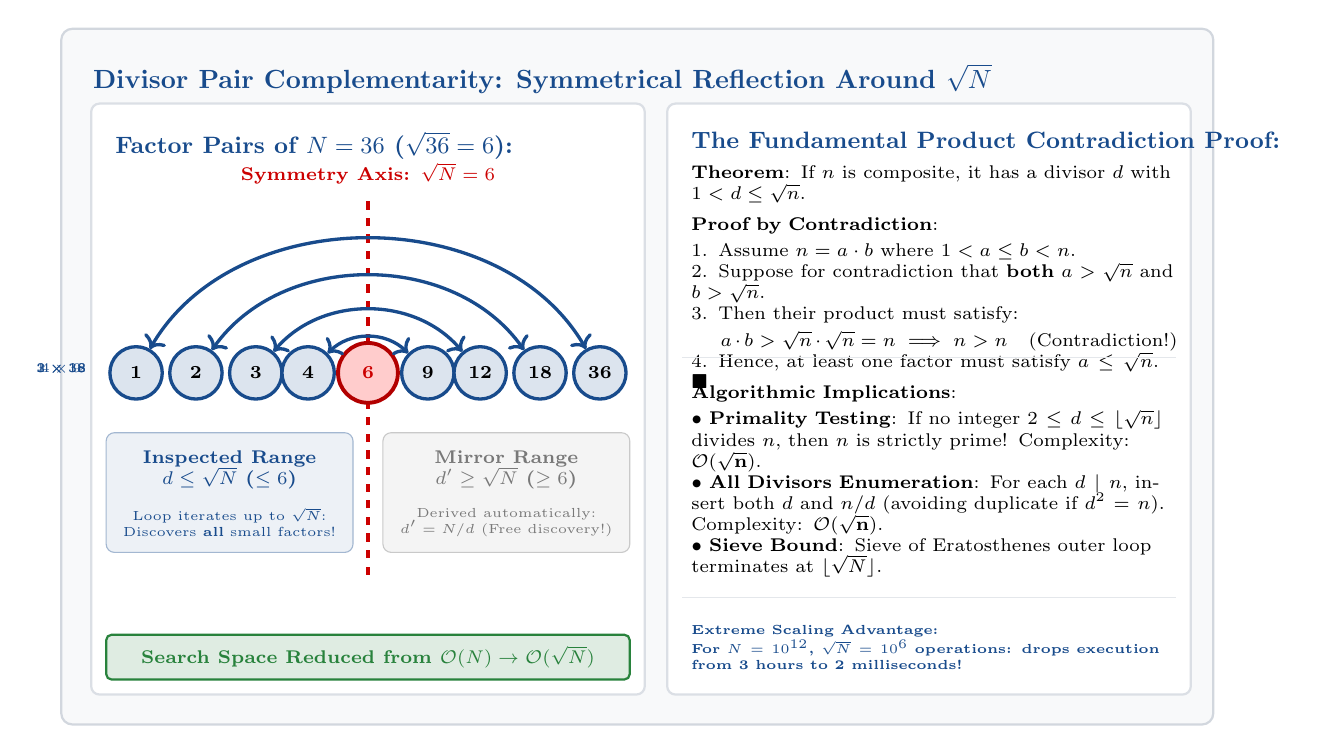
\begin{tikzpicture}[
    scale=0.95, every node/.style={transform shape},
    dNode/.style={circle, draw=primaryblue, fill=primaryblue!15, very thick, minimum size=0.7cm, font=\scriptsize\bfseries, align=center},
    pivotNode/.style={circle, draw=red!70!black, fill=red!20, line width=1.4pt, minimum size=0.8cm, font=\scriptsize\bfseries, text=red!80!black, align=center},
    card/.style={draw=codeframe, fill=codebg, rounded corners=4pt, thick}
]
    % Container Frame
    \draw[card] (0.0, -4.5) rectangle (15.4, 4.8);
    \node[anchor=north west, font=\bfseries\normalsize, text=primaryblue] at (0.3, 4.45) {Divisor Pair Complementarity: Symmetrical Reflection Around $\sqrt{N}$};

    % --- Left Panel: Arc Symmetry for N = 36 (x: 0.4 to 7.8) ---
    \draw[draw=codeframe!80, fill=white, rounded corners=3pt, thick] (0.4, -4.1) rectangle (7.8, 3.8);
    \node[anchor=north west, font=\small\bfseries, text=primaryblue] at (0.6, 3.55) {Factor Pairs of $N = 36$ ($\sqrt{36} = 6$):};

    % Central reflection axis line
    \draw[dashed, line width=1.3pt, red!80!black] (4.1, -2.5) -- (4.1, 2.5);
    \node[anchor=south, font=\scriptsize\bfseries, text=red!80!black] at (4.1, 2.6) {Symmetry Axis: $\sqrt{N} = 6$};

    % Divisor nodes placed along horizontal baseline y = 0.2
    % Left side (d <= 6): 1, 2, 3, 4, 6
    \node[dNode] (D1) at (1.0, 0.2) {1};
    \node[dNode] (D2) at (1.8, 0.2) {2};
    \node[dNode] (D3) at (2.6, 0.2) {3};
    \node[dNode] (D4) at (3.3, 0.2) {4};
    \node[pivotNode] (D6) at (4.1, 0.2) {6};

    % Right side (d > 6): 9, 12, 18, 36
    \node[dNode] (D9)  at (4.9, 0.2) {9};
    \node[dNode] (D12) at (5.6, 0.2) {12};
    \node[dNode] (D18) at (6.4, 0.2) {18};
    \node[dNode] (D36) at (7.2, 0.2) {36};

    % Complementary arcs connecting pairs
    \draw[<->, line width=1.2pt, primaryblue] (D4) to[bend left=45] (D9)
        node[midway, above=1pt, font=\tiny\bfseries] {$4 \times 9$};
    \draw[<->, line width=1.2pt, primaryblue] (D3) to[bend left=50] (D12)
        node[midway, above=1pt, font=\tiny\bfseries] {$3 \times 12$};
    \draw[<->, line width=1.2pt, primaryblue] (D2) to[bend left=55] (D18)
        node[midway, above=1pt, font=\tiny\bfseries] {$2 \times 18$};
    \draw[<->, line width=1.2pt, primaryblue] (D1) to[bend left=60] (D36)
        node[midway, above=1pt, font=\tiny\bfseries] {$1 \times 36$};

    % Regions
    \draw[draw=primaryblue!40, fill=primaryblue!8, rounded corners=3pt] (0.6, -2.2) rectangle (3.9, -0.6);
    \node[font=\scriptsize\bfseries, text=primaryblue, align=center] at (2.25, -1.1) {
        \textbf{Inspected Range}\\
        $d \le \sqrt{N}$ ($\le 6$)
    };
    \node[font=\tiny, text=primaryblue, align=center] at (2.25, -1.8) {
        Loop iterates up to $\sqrt{N}$:\\
        Discovers \textbf{all} small factors!
    };

    \draw[draw=codegray!40, fill=codegray!8, rounded corners=3pt] (4.3, -2.2) rectangle (7.6, -0.6);
    \node[font=\scriptsize\bfseries, text=codegray, align=center] at (5.95, -1.1) {
        \textbf{Mirror Range}\\
        $d' \ge \sqrt{N}$ ($\ge 6$)
    };
    \node[font=\tiny, text=codegray, align=center] at (5.95, -1.8) {
        Derived automatically:\\
        $d' = N / d$ (Free discovery!)
    };

    \draw[fill=codegreen!15, draw=codegreen, rounded corners=2pt, thick] (0.6, -3.9) rectangle (7.6, -3.3);
    \node[font=\scriptsize\bfseries, text=codegreen] at (4.1, -3.6) {Search Space Reduced from $\mathcal{O}(N) \to \mathcal{O}(\sqrt{N})$};

    % --- Right Panel: Mathematical Proof & Invariants (x: 8.1 to 15.1) ---
    \draw[draw=codeframe!80, fill=white, rounded corners=3pt, thick] (8.1, -4.1) rectangle (15.1, 3.8);
    \node[anchor=north west, font=\small\bfseries, text=primaryblue] at (8.3, 3.55) {The Fundamental Product Contradiction Proof:};

    \node[anchor=north west, font=\scriptsize, align=left, text width=6.5cm] at (8.3, 3.1) {
        \textbf{Theorem}: If $n$ is composite, it has a divisor $d$ with $1 < d \le \sqrt{n}$.\\[4pt]
        \textbf{Proof by Contradiction}:\\[2pt]
        1. Assume $n = a \cdot b$ where $1 < a \le b < n$.\\
        2. Suppose for contradiction that \textbf{both} $a > \sqrt{n}$ and $b > \sqrt{n}$.\\
        3. Then their product must satisfy:\\[2pt]
        \phantom{xx} $a \cdot b > \sqrt{n} \cdot \sqrt{n} = n \implies n > n \quad (\text{Contradiction!})$\\
        4. Hence, at least one factor must satisfy $a \le \sqrt{n}$. \ $\blacksquare$
    };

    \draw[draw=codeframe!60] (8.3, 0.4) -- (14.9, 0.4);

    \node[anchor=north west, font=\scriptsize, align=left, text width=6.5cm] at (8.3, 0.15) {
        \textbf{Algorithmic Implications}:\\[2pt]
        $\bullet$ \textbf{Primality Testing}: If no integer $2 \le d \le \lfloor\sqrt{n}\rfloor$ divides $n$, then $n$ is strictly prime! Complexity: $\mathbf{\mathcal{O}(\sqrt{n})}$.\\
        $\bullet$ \textbf{All Divisors Enumeration}: For each $d \mid n$, insert both $d$ and $n/d$ (avoiding duplicate if $d^2 = n$). Complexity: $\mathbf{\mathcal{O}(\sqrt{n})}$.\\
        $\bullet$ \textbf{Sieve Bound}: Sieve of Eratosthenes outer loop terminates at $\lfloor\sqrt{N}\rfloor$.
    };

    \draw[draw=codeframe!60] (8.3, -2.8) -- (14.9, -2.8);

    \node[anchor=north west, font=\tiny\bfseries, text=primaryblue, align=left, text width=6.5cm] at (8.3, -3.05) {
        Extreme Scaling Advantage:\\
        For $N = 10^{12}$, $\sqrt{N} = 10^6$ operations: drops execution from 3 hours to $\mathbf{2\text{ milliseconds}}$!
    };
\end{tikzpicture}}
\caption{Divisor complementary symmetry and the $\sqrt{N}$ reflection axis. Divisors occur in pairs $(d, N/d)$ across the central axis $\sqrt{N}$; finding all divisors or proving primality requires traversing strictly up to $\lfloor\sqrt{N}\rfloor$.}
\end{figure}

\newpage
\newpage
\newpage

\subsection[Diagram 40: Pascal's Triangle and Grid Lattice Paths]{Diagram 40: Pascal's Triangle Additive Pyramid \& Grid Lattice Paths $\binom{n}{k}$}

\breadcrumb{01.math_foundations.tex}{Section 2.2: Binomial Coefficients and Combinatorics}{Visualizes Pascal's identity $\binom{n}{k} = \binom{n-1}{k-1} + \binom{n-1}{k}$ and its structural equivalence to Manhattan grid lattice path routing.}

\diagramaudit{Agent (Antigravity)}{2026-10-12}{Constructed full-width 2-panel architecture: left panel combines Pascal's additive pyramid (rows 0--4) with a $2 \times 2$ Manhattan grid routing network; right panel proves combinatorial identities and outlines $\mathcal{O}(N^2)$ DP table construction.}

\begin{figure}[htbp]
\centering
\noindent\resizebox{\textwidth}{!}{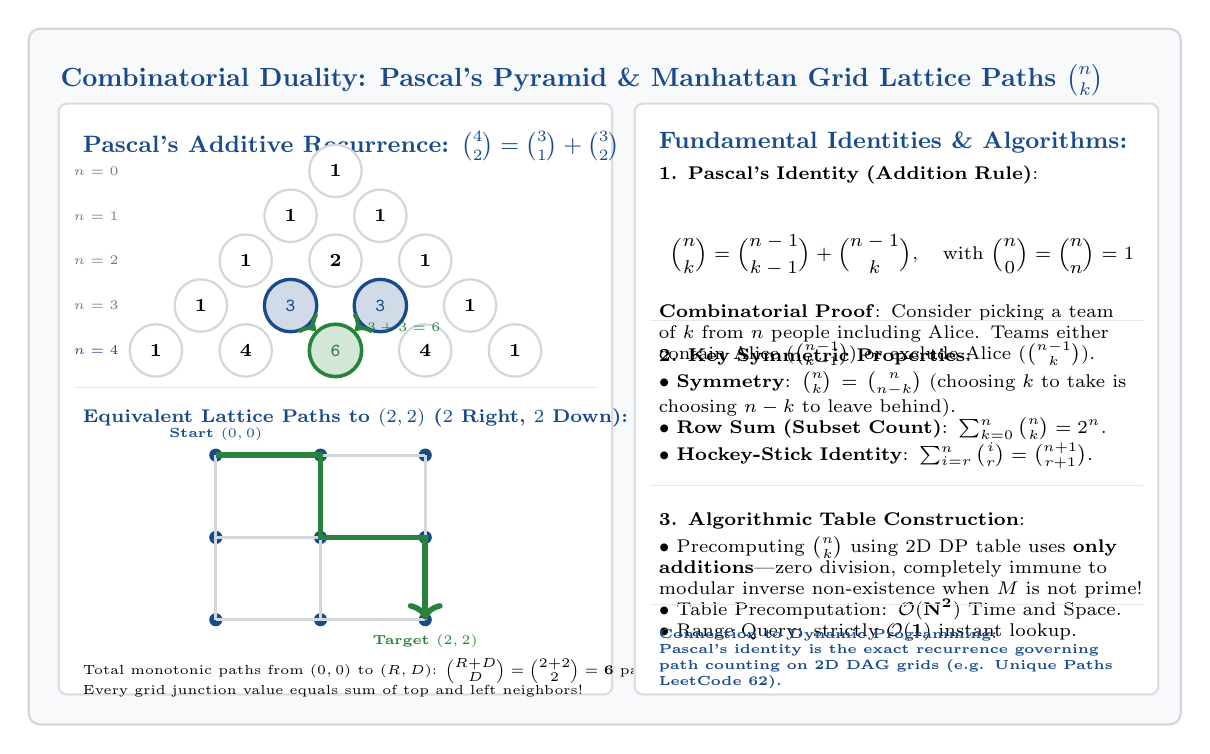
\begin{tikzpicture}[
    scale=0.95, every node/.style={transform shape},
    pNode/.style={circle, draw=codeframe, fill=white, thick, minimum size=0.7cm, font=\scriptsize\bfseries, align=center},
    sumNode/.style={circle, draw=codegreen, fill=codegreen!20, line width=1.3pt, minimum size=0.7cm, font=\scriptsize\bfseries\ttfamily, text=codegreen, align=center},
    srcNode/.style={circle, draw=primaryblue, fill=primaryblue!20, line width=1.2pt, minimum size=0.7cm, font=\scriptsize\bfseries\ttfamily, text=primaryblue, align=center},
    card/.style={draw=codeframe, fill=codebg, rounded corners=4pt, thick}
]
    % Container Frame
    \draw[card] (0.0, -4.5) rectangle (15.4, 4.8);
    \node[anchor=north west, font=\bfseries\normalsize, text=primaryblue] at (0.3, 4.45) {Combinatorial Duality: Pascal's Pyramid \& Manhattan Grid Lattice Paths $\binom{n}{k}$};

    % --- Left Panel: Pascal Triangle & Grid (x: 0.4 to 7.8) ---
    \draw[draw=codeframe!80, fill=white, rounded corners=3pt, thick] (0.4, -4.1) rectangle (7.8, 3.8);
    \node[anchor=north west, font=\small\bfseries, text=primaryblue] at (0.6, 3.55) {Pascal's Additive Recurrence: $\binom{4}{2} = \binom{3}{1} + \binom{3}{2}$};

    % Pascal Rows (Row 0 at y=3.0, down to Row 4 at y=0.6)
    % Row 0 (n=0): 1
    \node[pNode] at (4.1, 2.9) {1};

    % Row 1 (n=1): 1, 1
    \node[pNode] at (3.5, 2.3) {1};
    \node[pNode] at (4.7, 2.3) {1};

    % Row 2 (n=2): 1, 2, 1
    \node[pNode] at (2.9, 1.7) {1};
    \node[pNode] at (4.1, 1.7) {2};
    \node[pNode] at (5.3, 1.7) {1};

    % Row 3 (n=3): 1, 3, 3, 1
    \node[pNode] at (2.3, 1.1) {1};
    \node[srcNode] (P31) at (3.5, 1.1) {3};
    \node[srcNode] (P32) at (4.7, 1.1) {3};
    \node[pNode] at (5.9, 1.1) {1};

    % Row 4 (n=4): 1, 4, 6, 4, 1
    \node[pNode] at (1.7, 0.5) {1};
    \node[pNode] at (2.9, 0.5) {4};
    \node[sumNode] (P42) at (4.1, 0.5) {6};
    \node[pNode] at (5.3, 0.5) {4};
    \node[pNode] at (6.5, 0.5) {1};

    % Addition arrows: (P31) and (P32) -> (P42)
    \draw[->, line width=1.4pt, codegreen] (P31) -- (P42);
    \draw[->, line width=1.4pt, codegreen] (P32) -- (P42);
    \node[anchor=west, font=\tiny\bfseries, text=codegreen] at (4.4, 0.8) {$3 + 3 = 6$};

    % Row labels on left
    \node[font=\tiny\bfseries, text=codegray] at (0.9, 2.9) {$n=0$};
    \node[font=\tiny\bfseries, text=codegray] at (0.9, 2.3) {$n=1$};
    \node[font=\tiny\bfseries, text=codegray] at (0.9, 1.7) {$n=2$};
    \node[font=\tiny\bfseries, text=codegray] at (0.9, 1.1) {$n=3$};
    \node[font=\tiny\bfseries, text=primaryblue] at (0.9, 0.5) {$n=4$};

    % Bottom half of left panel: 2x2 Grid Lattice Path
    \draw[draw=codeframe!60] (0.6, 0.0) -- (7.6, 0.0);
    \node[anchor=north west, font=\scriptsize\bfseries, text=primaryblue] at (0.6, -0.15) {Equivalent Lattice Paths to $(2, 2)$ ($2$ Right, $2$ Down):};

    % 2x2 grid vertices: (2.2, -1.0) to (5.2, -3.2)
    % Vertices (r, c)
    \foreach \r in {0, 1, 2} {
        \foreach \c in {0, 1, 2} {
            \fill[primaryblue] (2.5 + \c*1.4, -0.9 - \r*1.1) circle (2.5pt);
        }
    }
    % Grid edges
    \foreach \r in {0, 1, 2} {
        \draw[line width=1.0pt, codeframe] (2.5, -0.9 - \r*1.1) -- (5.3, -0.9 - \r*1.1);
    }
    \foreach \c in {0, 1, 2} {
        \draw[line width=1.0pt, codeframe] (2.5 + \c*1.4, -0.9) -- (2.5 + \c*1.4, -3.1);
    }

    % One sample path in bold green: Start (0,0) -> (0,1) -> (1,1) -> (1,2) -> (2,2)
    \draw[->, line width=2.0pt, codegreen] (2.5, -0.9) -- (3.9, -0.9) -- (3.9, -2.0) -- (5.3, -2.0) -- (5.3, -3.1);

    % Start and End badges
    \node[above=2pt, font=\tiny\bfseries, text=primaryblue] at (2.5, -0.9) {Start $(0,0)$};
    \node[below=2pt, font=\tiny\bfseries, text=codegreen] at (5.3, -3.1) {Target $(2,2)$};

    \node[anchor=north west, font=\tiny, align=left] at (0.6, -3.5) {
        Total monotonic paths from $(0,0)$ to $(R, D)$: $\binom{R+D}{D} = \binom{2+2}{2} = \mathbf{6\text{ paths}}$.\\
        Every grid junction value equals sum of top and left neighbors!
    };

    % --- Right Panel: Combinatorial Invariants (x: 8.1 to 15.1) ---
    \draw[draw=codeframe!80, fill=white, rounded corners=3pt, thick] (8.1, -4.1) rectangle (15.1, 3.8);
    \node[anchor=north west, font=\small\bfseries, text=primaryblue] at (8.3, 3.55) {Fundamental Identities \& Algorithms:};

    \node[anchor=north west, font=\scriptsize, align=left, text width=6.5cm] at (8.3, 3.1) {
        \textbf{1. Pascal's Identity (Addition Rule)}:\\[2pt]
        $$\binom{n}{k} = \binom{n-1}{k-1} + \binom{n-1}{k}, \quad \text{with } \binom{n}{0} = \binom{n}{n} = 1$$
        \textbf{Combinatorial Proof}: Consider picking a team of $k$ from $n$ people including Alice. Teams either contain Alice ($\binom{n-1}{k-1}$) or exclude Alice ($\binom{n-1}{k}$).
    };

    \draw[draw=codeframe!60] (8.3, 0.9) -- (14.9, 0.9);

    \node[anchor=north west, font=\scriptsize, align=left, text width=6.5cm] at (8.3, 0.65) {
        \textbf{2. Key Symmetric Properties}:\\[2pt]
        $\bullet$ \textbf{Symmetry}: $\binom{n}{k} = \binom{n}{n-k}$ (choosing $k$ to take is choosing $n-k$ to leave behind).\\
        $\bullet$ \textbf{Row Sum (Subset Count)}: $\sum_{k=0}^n \binom{n}{k} = 2^n$.\\
        $\bullet$ \textbf{Hockey-Stick Identity}: $\sum_{i=r}^n \binom{i}{r} = \binom{n+1}{r+1}$.
    };

    \draw[draw=codeframe!60] (8.3, -1.3) -- (14.9, -1.3);

    \node[anchor=north west, font=\scriptsize, align=left, text width=6.5cm] at (8.3, -1.55) {
        \textbf{3. Algorithmic Table Construction}:\\[2pt]
        $\bullet$ Precomputing $\binom{n}{k}$ using 2D DP table uses \textbf{only additions}—zero division, completely immune to modular inverse non-existence when $M$ is not prime!\\
        $\bullet$ Table Precomputation: $\mathbf{\mathcal{O}(N^2)}$ Time and Space.\\
        $\bullet$ Range Query: strictly $\mathbf{\mathcal{O}(1)}$ instant lookup.
    };

    \draw[draw=codeframe!60] (8.3, -2.9) -- (14.9, -2.9);

    \node[anchor=north west, font=\tiny\bfseries, text=primaryblue, align=left, text width=6.5cm] at (8.3, -3.1) {
        Connection to Dynamic Programming:\\
        Pascal's identity is the exact recurrence governing path counting on 2D DAG grids (e.g. Unique Paths LeetCode 62).
    };
\end{tikzpicture}}
\caption{Pascal's triangle additive pyramid and Manhattan grid lattice path duality. Pascal's recurrence $\binom{n}{k} = \binom{n-1}{k-1} + \binom{n-1}{k}$ mirrors 2D grid path summation, allowing division-free $\mathcal{O}(N^2)$ precomputation.}
\end{figure}

\newpage
\newpage
\newpage

\subsection[Diagram 41: Brian Kernighan's Bit Stripping]{Diagram 41: Brian Kernighan's Algorithm: Lowest 1-Bit Stripping via $x \mathbin{\&} (x - 1)$}

\breadcrumb{12.bit_manipulation.tex}{Section 2.3: Bitwise Tricks and Classical Techniques}{Visualizes borrow propagation during subtraction and the zeroing of the least significant set bit in $\mathcal{O}(k)$ iterations.}

\diagramaudit{Agent (Antigravity)}{2026-10-12}{Constructed full-width 2-panel architecture: left panel shows 8-bit register traces for x=12 and x=8 with borrow inversion; right panel formalizes prefix bit invariance, power-of-two tests, and O(k) popcount guarantees.}

\begin{figure}[htbp]
\centering
\noindent\resizebox{\textwidth}{!}{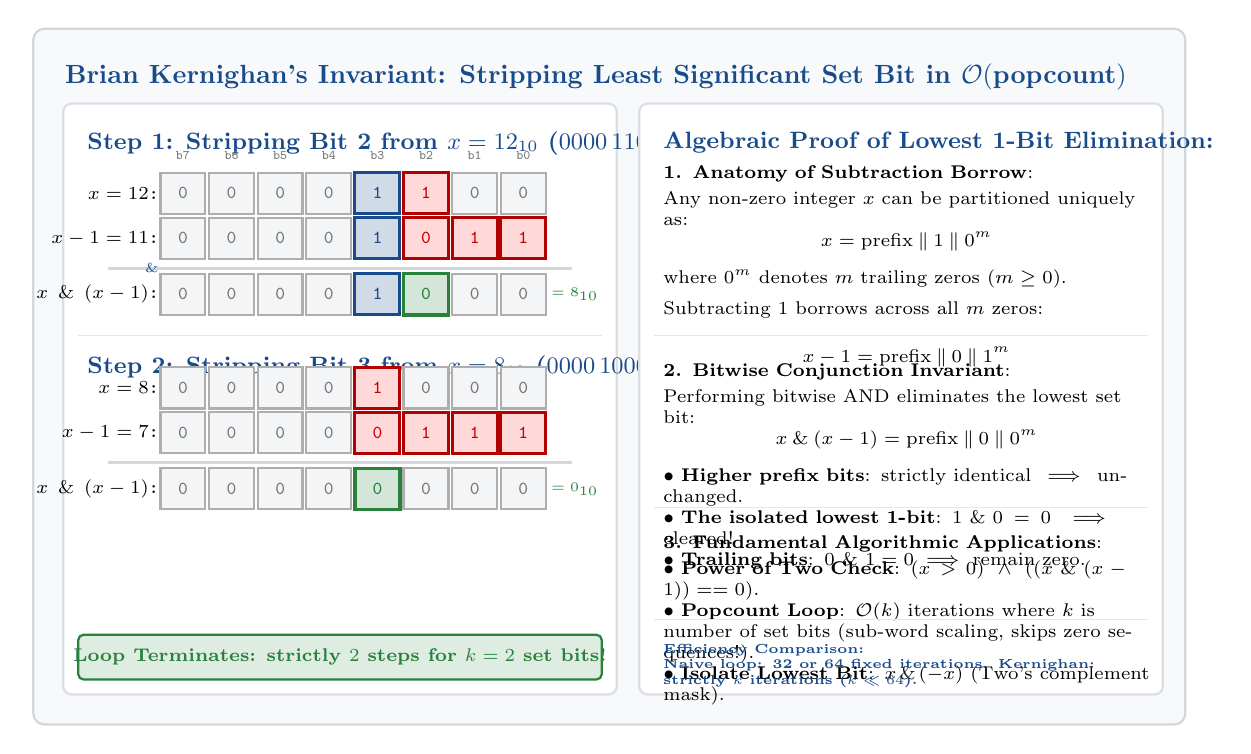
\begin{tikzpicture}[
    scale=0.95, every node/.style={transform shape},
    bCell/.style={draw=codeframe, fill=white, thick, minimum width=0.6cm, minimum height=0.55cm, font=\scriptsize\ttfamily, align=center},
    bZero/.style={draw=codegray!60, fill=codeframe!25, thick, minimum width=0.6cm, minimum height=0.55cm, font=\scriptsize\ttfamily, text=codegray, align=center},
    bOne/.style={draw=primaryblue, fill=primaryblue!20, line width=1.1pt, minimum width=0.6cm, minimum height=0.55cm, font=\scriptsize\bfseries\ttfamily, text=primaryblue, align=center},
    bFlip/.style={draw=red!70!black, fill=red!15, line width=1.1pt, minimum width=0.6cm, minimum height=0.55cm, font=\scriptsize\bfseries\ttfamily, text=red!80!black, align=center},
    bStrip/.style={draw=codegreen, fill=codegreen!20, line width=1.2pt, minimum width=0.6cm, minimum height=0.55cm, font=\scriptsize\bfseries\ttfamily, text=codegreen, align=center},
    card/.style={draw=codeframe, fill=codebg, rounded corners=4pt, thick}
]
    % Container Frame
    \draw[card] (0.0, -4.5) rectangle (15.4, 4.8);
    \node[anchor=north west, font=\bfseries\normalsize, text=primaryblue] at (0.3, 4.45) {Brian Kernighan's Invariant: Stripping Least Significant Set Bit in $\mathcal{O}(\text{popcount})$};

    % --- Left Panel: Register Bitwise Arithmetic (x: 0.4 to 7.8) ---
    \draw[draw=codeframe!80, fill=white, rounded corners=3pt, thick] (0.4, -4.1) rectangle (7.8, 3.8);
    \node[anchor=north west, font=\small\bfseries, text=primaryblue] at (0.6, 3.55) {Step 1: Stripping Bit 2 from $x = 12_{10}$ ($0000\,1100_2$)};

    % Bit labels (7 down to 0) at y = 3.1
    \foreach \b/\idx in {0/7, 1/6, 2/5, 3/4, 4/3, 5/2, 6/1, 7/0} {
        \node[font=\tiny\ttfamily, text=codegray] at (2.0 + \b*0.65, 3.1) {b\idx};
    }

    % Row 1: x = 12 (0000 1100) at y = 2.6
    \node[anchor=east, font=\scriptsize\ttfamily] at (1.8, 2.6) {$x = 12$:};
    \foreach \b/\val in {0/0, 1/0, 2/0, 3/0} { \node[bZero] at (2.0 + \b*0.65, 2.6) {\val}; }
    \node[bOne]  at (2.0 + 4*0.65, 2.6) {1};
    \node[bFlip] at (2.0 + 5*0.65, 2.6) {1};
    \node[bZero] at (2.0 + 6*0.65, 2.6) {0};
    \node[bZero] at (2.0 + 7*0.65, 2.6) {0};

    % Row 2: x - 1 = 11 (0000 1011) at y = 2.0
    \node[anchor=east, font=\scriptsize\ttfamily] at (1.8, 2.0) {$x - 1 = 11$:};
    \foreach \b/\val in {0/0, 1/0, 2/0, 3/0} { \node[bZero] at (2.0 + \b*0.65, 2.0) {\val}; }
    \node[bOne]  at (2.0 + 4*0.65, 2.0) {1};
    \node[bFlip] at (2.0 + 5*0.65, 2.0) {0};
    \node[bFlip] at (2.0 + 6*0.65, 2.0) {1};
    \node[bFlip] at (2.0 + 7*0.65, 2.0) {1};

    % Horizontal line for AND operation
    \draw[line width=1.1pt, codeframe] (1.0, 1.6) -- (7.2, 1.6);
    \node[anchor=east, font=\tiny\bfseries, text=primaryblue] at (1.8, 1.6) {$\&$};

    % Row 3: x & (x-1) = 8 (0000 1000) at y = 1.25
    \node[anchor=east, font=\scriptsize\ttfamily] at (1.8, 1.25) {$x \ \& \ (x-1)$:};
    \foreach \b/\val in {0/0, 1/0, 2/0, 3/0} { \node[bZero] at (2.0 + \b*0.65, 1.25) {\val}; }
    \node[bOne]   at (2.0 + 4*0.65, 1.25) {1};
    \node[bStrip] at (2.0 + 5*0.65, 1.25) {0};
    \node[bZero]  at (2.0 + 6*0.65, 1.25) {0};
    \node[bZero]  at (2.0 + 7*0.65, 1.25) {0};
    \node[anchor=west, font=\tiny\bfseries, text=codegreen] at (6.8, 1.25) {$= 8_{10}$};

    % Step 2 at y = 0.3 down to -1.5
    \draw[draw=codeframe!60] (0.6, 0.7) -- (7.6, 0.7);
    \node[anchor=north west, font=\small\bfseries, text=primaryblue] at (0.6, 0.55) {Step 2: Stripping Bit 3 from $x = 8_{10}$ ($0000\,1000_2$)};

    % Row 4: x = 8 (0000 1000) at y = 0.0
    \node[anchor=east, font=\scriptsize\ttfamily] at (1.8, 0.0) {$x = 8$:};
    \foreach \b/\val in {0/0, 1/0, 2/0, 3/0} { \node[bZero] at (2.0 + \b*0.65, 0.0) {\val}; }
    \node[bFlip] at (2.0 + 4*0.65, 0.0) {1};
    \foreach \b/\val in {5/0, 6/0, 7/0} { \node[bZero] at (2.0 + \b*0.65, 0.0) {\val}; }

    % Row 5: x - 1 = 7 (0000 0111) at y = -0.6
    \node[anchor=east, font=\scriptsize\ttfamily] at (1.8, -0.6) {$x - 1 = 7$:};
    \foreach \b/\val in {0/0, 1/0, 2/0, 3/0} { \node[bZero] at (2.0 + \b*0.65, -0.6) {\val}; }
    \node[bFlip] at (2.0 + 4*0.65, -0.6) {0};
    \foreach \b/\val in {5/1, 6/1, 7/1} { \node[bFlip] at (2.0 + \b*0.65, -0.6) {\val}; }

    % Horizontal line for AND
    \draw[line width=1.1pt, codeframe] (1.0, -1.0) -- (7.2, -1.0);

    % Row 6: x & (x-1) = 0 (0000 0000) at y = -1.35
    \node[anchor=east, font=\scriptsize\ttfamily] at (1.8, -1.35) {$x \ \& \ (x-1)$:};
    \foreach \b/\val in {0/0, 1/0, 2/0, 3/0} { \node[bZero] at (2.0 + \b*0.65, -1.35) {\val}; }
    \node[bStrip] at (2.0 + 4*0.65, -1.35) {0};
    \foreach \b/\val in {5/0, 6/0, 7/0} { \node[bZero] at (2.0 + \b*0.65, -1.35) {\val}; }
    \node[anchor=west, font=\tiny\bfseries, text=codegreen] at (6.8, -1.35) {$= 0_{10}$};

    \draw[fill=codegreen!15, draw=codegreen, rounded corners=2pt, thick] (0.6, -3.9) rectangle (7.6, -3.3);
    \node[font=\scriptsize\bfseries, text=codegreen] at (4.1, -3.6) {Loop Terminates: strictly $2$ steps for $k = 2$ set bits!};

    % --- Right Panel: Structural Theory & Invariants (x: 8.1 to 15.1) ---
    \draw[draw=codeframe!80, fill=white, rounded corners=3pt, thick] (8.1, -4.1) rectangle (15.1, 3.8);
    \node[anchor=north west, font=\small\bfseries, text=primaryblue] at (8.3, 3.55) {Algebraic Proof of Lowest 1-Bit Elimination:};

    \node[anchor=north west, font=\scriptsize, align=left, text width=6.5cm] at (8.3, 3.1) {
        \textbf{1. Anatomy of Subtraction Borrow}:\\[2pt]
        Any non-zero integer $x$ can be partitioned uniquely as:
        $$x = \text{prefix} \mathbin{\parallel} 1 \mathbin{\parallel} 0^m$$
        where $0^m$ denotes $m$ trailing zeros ($m \ge 0$).\\[4pt]
        Subtracting $1$ borrows across all $m$ zeros:
        $$x - 1 = \text{prefix} \mathbin{\parallel} 0 \mathbin{\parallel} 1^m$$
    };

    \draw[draw=codeframe!60] (8.3, 0.7) -- (14.9, 0.7);

    \node[anchor=north west, font=\scriptsize, align=left, text width=6.5cm] at (8.3, 0.45) {
        \textbf{2. Bitwise Conjunction Invariant}:\\[2pt]
        Performing bitwise AND eliminates the lowest set bit:
        $$x \mathbin{\&} (x - 1) = \text{prefix} \mathbin{\parallel} 0 \mathbin{\parallel} 0^m$$
        $\bullet$ \textbf{Higher prefix bits}: strictly identical $\implies$ unchanged.\\
        $\bullet$ \textbf{The isolated lowest 1-bit}: $1 \ \& \ 0 = 0 \implies$ cleared!\\
        $\bullet$ \textbf{Trailing bits}: $0 \ \& \ 1 = 0 \implies$ remain zero.
    };

    \draw[draw=codeframe!60] (8.3, -1.6) -- (14.9, -1.6);

    \node[anchor=north west, font=\scriptsize, align=left, text width=6.5cm] at (8.3, -1.85) {
        \textbf{3. Fundamental Algorithmic Applications}:\\[2pt]
        $\bullet$ \textbf{Power of Two Check}: $(x > 0) \ \land \ ((x \ \& \ (x - 1)) == 0)$.\\
        $\bullet$ \textbf{Popcount Loop}: $\mathcal{O}(k)$ iterations where $k$ is number of set bits (sub-word scaling, skips zero sequences!).\\
        $\bullet$ \textbf{Isolate Lowest Bit}: $x \mathbin{\&} (-x)$ (Two's complement mask).
    };

    \draw[draw=codeframe!60] (8.3, -3.1) -- (14.9, -3.1);

    \node[anchor=north west, font=\tiny\bfseries, text=primaryblue, align=left, text width=6.5cm] at (8.3, -3.3) {
        Efficiency Comparison:\\
        Naive loop: 32 or 64 fixed iterations. Kernighan: strictly $k$ iterations ($k \ll 64$).
    };
\end{tikzpicture}}
\caption{Brian Kernighan's algorithm for lowest set-bit elimination. Subtraction borrows across trailing zeros, transforming $x = \text{prefix} \parallel 1 \parallel 0^m$ into $x - 1 = \text{prefix} \parallel 0 \parallel 1^m$ and zeroing the lowest set bit in $\mathcal{O}(\text{popcount})$ operations.}
\end{figure}


\newpage
\section{Technical Monograph Integration Plan}
% ============================================================================

To fully elevate the repository's monographs to world-class pedagogical visual standards, the 33 newly designed diagrams in this 41-diagram gallery should be systematically integrated into their respective parent \texttt{.tex} source documents in an upcoming integration phase:

\begin{enumerate}
    \item \textbf{High-Priority Broken Placeholders}:
    Immediate integration is required for the empty diagram blocks in:
    \begin{itemize}
        \item \texttt{00.problem\_solving\_guide.tex} (Diagram 3 triage tree at lines 113--119).
        \item \texttt{02.modular\_arithmetic.tex} (Diagram 5 clock face at line 110).
        \item \texttt{03.number\_theory.tex} (Diagram 6 Sieve matrix at line 390).
        \item \texttt{05.recursion\_and\_backtracking.tex} (Diagram 11 Fibonacci tree at line 131; Diagram 12 Backtracking tree at line 282).
        \item \texttt{07.graph\_algorithms.tex} (Diagram 15 representation matrix at lines 177--179).
    \end{itemize}
    \item \textbf{Foundational Intuition Additions}:
    Embed into target monographs:
    \begin{itemize}
        \item \texttt{00.cpp\_reference.tex}: Diagram 1 (Stack vs Heap) and Diagram 2 (Vector Doubling).
        \item \texttt{01.combinatorics\_permutations.tex}: Diagram 4 (Stars and Bars).
        \item \texttt{03.number\_theory.tex}: Diagram 7 (Euclidean Tiling).
        \item \texttt{04.sequences\_and\_series.tex}: Diagrams 8 and 9 (Prefix Sums and Difference Arrays).
        \item \texttt{08.binary\_search.tex}: Diagrams 19 and 20 (Interval Halving and Predicate Monotonicity).
    \end{itemize}
    \item \textbf{Advanced Algorithmic Additions}:
    Embed into target monographs:
    \begin{itemize}
        \item \texttt{06.dynamic\_programming.tex}: Diagrams 13 and 14 (1D Tape and 2D Grid DP), Diagram 33 (0/1 Knapsack Space Optimization), and Diagram 34 (LCS 2D State Matrix Reconstruction).
        \item \texttt{07.graph\_algorithms.tex}: Diagrams 16, 17, and 18 (BFS Wavefront, Dijkstra, DSU), Diagram 35 (Kahn's DAG Topological Sorting), and Diagram 36 (Bipartite 2-Coloring Contradiction).
        \item \texttt{08.binary\_search.tex}: Diagram 37 (Rotated Sorted Array Discontinuity Bifurcation).
        \item \texttt{09.string\_algorithms.tex}:\\ Diagram 29 (Trie Vector Pool Layout), Diagram 30 (KMP $\pi$ Fallback Transitions), and Diagram 31 (Rabin-Karp Rolling Hash Shift).
        \item \texttt{01.combinatorics\_permutations.tex}:\\ Diagram 40 (Pascal's Triangle Additive Pyramid and Lattice Paths).
        \item \texttt{02.modular\_arithmetic.tex}:\\ Diagram 38 (Binary Exponentiation Repeated Squaring Tree).
        \item \texttt{03.number\_theory.tex}:\\ Diagram 39 (Divisor Complementary Symmetry across $\sqrt{N}$).
        \item \texttt{04.sequences\_and\_series.tex}:\\ Diagram 32 (2D Prefix Sum Subgrid Inclusion-Exclusion).
        \item \texttt{12.bit\_manipulation\_and\_bitmasks.tex}:\\ Diagram 41 (Brian Kernighan's Lowest Set-Bit Stripping).
    \end{itemize}
\end{enumerate}

% --- Version History (always the last section of the document) ---
\section*{Version History}
\addcontentsline{toc}{section}{Version History}

\noindent
\begin{tabularx}{\textwidth}{|l|X|}
\hline
\textbf{Date} & \textbf{Change} \\ \hline
2026-10-11 & Document created. Exhaustive 12-module visual audit completed, missing placeholder inventory established, and 24-diagram unified TikZ gallery constructed with destination breadcrumbs. \\ \hline
2026-10-11 & Fixed Diagram 4 Stars-and-Bars condition logic, migrated audit table to xltabular, eliminated overfull boxes, and resolved font warnings. \\ \hline
2026-10-11 & Completed comprehensive visual review pass across all 24 diagrams. Redesigned all diagrams to span full page width ($\approx 15.5\text{ cm}$), harmonized color palette with code blocks (\texttt{primaryblue}, \texttt{codebg}, \texttt{codeframe}, \texttt{codegreen}, \texttt{codeblue}, \texttt{codegray}), eliminated all label/edge collisions and overlapping text, and established detailed mathematical and algorithmic trace panels. \\ \hline
2026-10-11 & Completed rigorous skeptical visual review and collision audit: eliminated text overlaps and margin overflows across Diagrams 2, 3, 4, 5, 7, 8, 9, 10, 11, 12, 13, 14, 15, 17, 18, 21, and 22; re-spaced nodes, calibrated arrow routing, and verified layout fidelity with \texttt{pdftoppm}. \\ \hline
2026-10-11 & Incorporated per-diagram review and audit tables across all 24 diagrams with reviewer attribution (Agent Antigravity), timestamp, and granular inspection/change log detailing exact geometry, routing, and invariant fixes. \\ \hline
2026-10-11 & Updated per-diagram audit table headers to Reviewer (Human/Agent) and calibrated TikZ diagram bounding boxes to eliminate all margin overflow warnings. \\ \hline
2026-10-12 & Integrated Module 12 (Bit Manipulation and Bitmasks) visual architecture: added Diagrams 25--28 (Integer Anatomy, LSB Isolation, Prefix XOR Cancellation, and Submask Enumeration Lattice) with breadcrumbs and audit logs. \\ \hline
2026-10-12 & Repository-wide visual expansion and audit complete: designed and integrated 13 publication-grade TikZ diagrams (Diagrams 29--41) covering Module 09 (Trie Prefix Tree, KMP Fallback Automaton, Rabin-Karp Rolling Hash Shift) and core monograph paradigms (2D Prefix Sum Inclusion-Exclusion, 0/1 Knapsack Space Compression, LCS 2D State Matrix, Kahn's DAG Topological Sort, Bipartite 2-Coloring Contradiction, Rotated Sorted Array Binary Search, Binary Exponentiation Tree, Divisor Reflection Axis across $\sqrt{N}$, Pascal Additive Lattice Paths, and Brian Kernighan's Bit Stripping); gallery expanded from 28 to 41 full-width standalone diagrams with destination breadcrumbs and audit tables. \\ \hline
\end{tabularx}

\end{document}
